% =====================================================================
%  Sections 3 (Method) and 4 (Experiments), English
%  acmart [sigconf,nonacm]; compiles with pdfLaTeX, XeLaTeX or LuaLaTeX
%
%  Include with: % =====================================================================
%  Sections 3 (Method) and 4 (Experiments), English
%  acmart [sigconf,nonacm]; compiles with pdfLaTeX, XeLaTeX or LuaLaTeX
%
%  Include with: % =====================================================================
%  Sections 3 (Method) and 4 (Experiments), English
%  acmart [sigconf,nonacm]; compiles with pdfLaTeX, XeLaTeX or LuaLaTeX
%
%  Include with: % =====================================================================
%  Sections 3 (Method) and 4 (Experiments), English
%  acmart [sigconf,nonacm]; compiles with pdfLaTeX, XeLaTeX or LuaLaTeX
%
%  Include with: \input{sections-method-experiments-en}
%  Required packages: booktabs, graphicx, amsmath, array, url
%  Figure path: ../figures_v2/  (output of scripts/make_paper_figures.py)
%  Additional references: merge paper-refs-additional.bib
% =====================================================================

\section{Method}
\label{sec:method}

\subsection{Setup: Symmetric Estimation}
\label{sec:setup}

Let the set of investor types be
$\mathcal{I}=\{\text{foreign},\text{institutional},\text{retail}\}$. Each type is
treated as an agent whose observed daily order flow reveals a latent reward
defined over interpretable market state features.

\paragraph{Continuous action}
Writing $V^{buy}_{i,t}$ and $V^{sell}_{i,t}$ for the daily gross buy and gross
sell value of type $i$, we define the action as
\begin{equation}
u_{i,t}=\frac{V^{buy}_{i,t}-V^{sell}_{i,t}}
             {V^{buy}_{i,t}+V^{sell}_{i,t}}\in[-1,1].
\label{eq:action}
\end{equation}
Because the denominator is the type's own gross turnover rather than
market-wide turnover, $u_{i,t}$ measures whether buying or selling dominated
\emph{within} that type, giving a common scale that is unaffected by
differences in trading size across types. Using a continuous intensity rather
than a binary buy/sell label preserves the magnitude information that
dichotomization discards.

\paragraph{Symmetry}
All three types receive the same state features $x_{i,t}\in\mathbb{R}^{3}$, the
same market context $C_t\in\mathbb{R}^{2}$, and the same model form. No type is
assigned a different feature a priori; only the parameters
$\theta_i=(\beta_i,B_i,\alpha_i)$ are estimated separately on each type's own
data. Any difference that appears in the results is therefore learned from the
data rather than imposed by design, and this symmetry is what licenses direct
comparison of coefficients across types.

\paragraph{Timing}
The training sample is $(x_{i,t},C_t,a_{i,t+1})$ with $a_{i,t+1}=u_{i,t+1}$. A
state built from day-$t$ closing prices and order flow explains day-$t+1$
behaviour, so no future trade enters the features. Momentum and underwater use
day-$t$ information while the herding feature uses day $t-1$. Since the target
is day-$t+1$ behaviour, day-$t$ information is also available; the extra lag on
herding is therefore not an information constraint but a design choice that
keeps the same-day accounting offset between types out of the predictor set
(Figure~\ref{fig:crossinv}).

\subsection{Reward Features}
\label{sec:features}

All three features are standardized using statistics fitted on the training
indices of each validation split only. Every coefficient reported below is
therefore read as the effect of a one-standard-deviation move of that feature
within the training window.

\paragraph{(F1) Medium-term momentum}
With adjusted (or fallback) closing price $P_t$,
\begin{equation}
x^{mom}_{i,t}=\log\!\left(\frac{P_t}{P_{t-20}}\right).
\label{eq:momentum}
\end{equation}
Twenty trading days is a pre-specified window of roughly one month, chosen to
damp daily price noise while still expressing a medium-term trend linked to
next-day behaviour. It is a design value for interpretability, not a value tuned
on the data. A positive coefficient indicates trend following and a negative one
contrarian trading; the sign expectation follows prior work on type-specific
momentum trading~\cite{grinblatt2000investment,choe1999foreign}.

\paragraph{(F2) Herding}
The cross-sectional average of the previous day's actions of the two types other
than $i$:
\begin{equation}
x^{herd}_{i,t}=\frac{u_{j,t-1}+u_{k,t-1}}{2},\qquad j,k\neq i.
\label{eq:herd}
\end{equation}
Note that this is an average across the two other types at one point in time,
not a time average. A 20-day moving average would measure a month of cumulative
flow pressure rather than an immediate response, so we focus on the previous
day. A positive coefficient means moving with the previous day's direction of
the other types, a negative one means moving against it. The sign expectation
follows the institutional herding
literature~\cite{lakonishok1992impact}; note however that this literature
measures herding \emph{within} the institutional group, whereas
Equation~\eqref{eq:herd} measures a relation \emph{between} types
(\S\ref{sec:construct}).

\paragraph{(F3) Underwater gap relative to average cost}
With a per-type average-cost proxy $\bar P_{i,t}$ and the day's gross-trade VWAP
$P^{vwap}_{i,t}$,
\begin{equation}
x^{uw}_{i,t}=\max\!\left(
\frac{\bar P_{i,t}-P^{vwap}_{i,t}}{\bar P_{i,t}},\,0\right).
\label{eq:underwater}
\end{equation}
Truncation at zero makes the feature active only when the traded price sits
below the average-cost proxy, so the variable is reference-point dependent by
construction. The average cost is obtained by recursively updating an effective
inventory from gross buy and sell quantities and values: the previous day's
inventory is multiplied by a forgetting factor $\rho=0.98$ to damp the influence
of old trades, and sales do not change the average cost of the remaining
position. With $\rho=0.98$ the half-life is about 34 trading days and roughly
66.8\% remains after 20, so the feature emphasises the trading memory of the
past one to two months; this value was also not tuned on the data. A positive
coefficient means stronger next-day buying below the average cost, and the sign
expectation follows the disposition-effect
literature~\cite{shefrin1985disposition,odean1998investors}.

The proxy is constructed from aggregate flow rather than actual account
holdings. Buys and sells executed by different accounts within the same type
net out, so the notion of a ``representative investor's average cost'' is itself
an approximation. The coefficient on $x^{uw}$ therefore cannot be read as a
direct test of the disposition effect.

\subsection{Market Context}
\label{sec:context}

The context consists of two variables: (C1) the one-day KOSPI200 return $r_t$,
and (C2) the KRW/USD exchange rate level
\begin{equation}
z_t=\frac{\log e_t-\mu_{t-1,252}}{\sigma_{t-1,252}},
\label{eq:fxcontext}
\end{equation}
where the current rate is used but the mean and standard deviation are computed
only through $t-1$ over 252 trading days. Both contexts are likewise
re-standardized on the training indices of each split, so their coefficients
read as the effect of a one-standard-deviation move within the training window.

Context and reward features are not independent. Because Samsung Electronics
carries a large weight in the KOSPI200, stock momentum overlaps with the market
return, and feature--context correlations range from $-0.29$ to $0.22$
(Figure~\ref{fig:featcorr}). Individual coefficients are therefore conditional
associations given the other terms and should not be read as causal magnitudes
in isolation.

\subsection{Myopic Reward, Policy, and the Reduction to Lasso}
\label{sec:model}

\paragraph{Latent action score}
Define the action score of type $i$ at time $t$ as
\begin{equation}
q_{i,t}=(\beta_i+B_iC_t)^{\top}x_{i,t}+\alpha_i^{\top}C_t,
\label{eq:score}
\end{equation}
where $\beta_i\in\mathbb{R}^{3}$ is the baseline reward weight at average
context, $B_i\in\mathbb{R}^{3\times 2}$ the feature--context interaction, and
$\alpha_i\in\mathbb{R}^{2}$ the direct context main effect. The $\alpha$ term is
a level effect that shifts behaviour even when the stock features are at their
means; the $B$ term is a slope effect that changes sensitivity to each feature
across market conditions. Including interaction terms while omitting the
lower-order term $C_t$ is a standard specification error, so the inclusion of
$\alpha$ is required by the specification rather than something to be justified
empirically.

\paragraph{Myopic concave reward}
The one-step reward for a continuous action $a$ is
\begin{equation}
R_i(x,C,a)=q_{i,t}\,a-\frac{\kappa}{2}a^{2}.
\label{eq:reward}
\end{equation}
The quadratic term imposes a symmetric cost on large net buying and net selling
and makes the reward concave in the action, which permits an interior solution.
Without it, maximizing over $[-1,1]$ would return $\pm1$ almost always depending
only on the sign of $q$, and the \emph{intensity} of behaviour could not be
reproduced. Maximizing Equation~\eqref{eq:reward} over $a$ yields the closed-form
policy
\begin{equation}
a^{*}_{i,t+1}=\mathrm{clip}\!\left(\frac{q_{i,t}}{\kappa},-1,1\right).
\label{eq:policy}
\end{equation}
The curvature $\kappa$ is fixed at one for identification. With $\kappa=2$ the
same $q$ would halve the action size, but re-estimation would double the
coefficients of $q$ and reproduce the same behaviour; $\kappa=1$ therefore fixes
the units of the reward and the coefficients rather than asserting that the
empirical curvature equals one.

\paragraph{Estimation}
The training objective for each type on its training set $\mathcal{D}_i$ is
\begin{equation}
\min_{\theta_i}\ \frac{1}{|\mathcal{D}_i|}
\sum_{t\in\mathcal{D}_i}\bigl(a^{*}_{i,t+1}-a_{i,t+1}\bigr)^{2}
+\lambda_i\lVert\theta_i\rVert_1,
\label{eq:loss}
\end{equation}
optimized independently per type with Adam~\cite{kingma2015adam}.

\begin{proposition}[Reduction to Lasso]
\label{prop:lasso}
Let
$z_{i,t}=[\,x_{i,t};\ \mathrm{vec}(x_{i,t}C_t^{\top});\ C_t\,]\in\mathbb{R}^{11}$
and $\theta_i=[\,\beta_i;\ \mathrm{vec}(B_i);\ \alpha_i\,]$, so that
Equation~\eqref{eq:score} reads $q_{i,t}=\theta_i^{\top}z_{i,t}$. If
$|q_{i,t}|\le 1$ throughout the training sample, the clip in
Equation~\eqref{eq:policy} never binds, $a^{*}=q$, and
Equation~\eqref{eq:loss} becomes
\begin{equation}
\min_{\theta_i}\ \frac{1}{|\mathcal{D}_i|}
\sum_{t}\bigl(\theta_i^{\top}z_{i,t}-a_{i,t+1}\bigr)^{2}
+\lambda_i\lVert\theta_i\rVert_1,
\label{eq:lasso}
\end{equation}
which is exactly an $L_1$-penalized (Lasso) regression of next-day net-buying
intensity on the expanded state feature $z$.
\end{proposition}

Under a myopic concave reward with $\kappa=1$, ``recovering a preference'' and
``regressing order flow'' are therefore numerically indistinguishable.
Figure~\ref{fig:saturation} shows that the premise of
Proposition~\ref{prop:lasso} in fact holds in our sample: for all three types the
distribution of the latent action score sits far inside the action bounds
$\pm1$ (the maximum $|q|$ is 0.842 for foreign, 0.587 for retail and 0.135 for
institutional investors), and the saturation rate is exactly zero in all 45
splits.

\paragraph{Why we do not hide the reduction}
This coincidence is not a weakness of the method but a logical consequence of
the myopia assumption. If the agent looks only one step ahead, today's action
does not affect anything beyond tomorrow, so there is no future to look toward
and \emph{what the agent wants} (the reward) collapses onto \emph{what the agent
does} (the policy). Applying the stochastic policy of maximum-entropy
IRL~\cite{ziebart2008maximum}, $\pi(a\mid x,C)\propto\exp(R/\tau)$, to
Equation~\eqref{eq:reward} makes $\pi$ a truncated normal with mean $q$ and
variance $\tau$, whose maximum-likelihood point estimate coincides with
Equation~\eqref{eq:lasso}. The reduction is thus a property of the myopic,
quadratic-reward setting in general, not an artefact of one implementation.

The distinctive value of the inverse reinforcement learning formulation lies in
the extension path. Once state dynamics and multi-period value are introduced,
the reward separates from the policy and leads to a structural recovery that
regression cannot reach. This paper is the first step on that path, and it adds
interpretation and validation on top of an explicitly stated set of conditions.

\subsection{Validation Protocol}
\label{sec:protocol}

Rather than stopping at the sign and magnitude of the recovered coefficients, we
apply four stages.

\begin{description}
\item[(V1) Out-of-sample stability under CPCV] We use combinatorial purged
cross-validation~\cite{lopez2018advances} with ten temporal folds of which two
serve as test folds, giving $\binom{10}{2}=45$ splits, a one-day purge and a
five-day embargo between training and test, and all standardization fitted on
training indices only. We report the fraction of splits in which the dominant
sign appears (sign consistency), but because the splits share observations we
interpret sign consistency only as a stability indicator, never as an
independent-sample $p$-value.

\item[(V2) Calendar-month block bootstrap] To address the fact that sign
consistency is not a test, we partition the sample into calendar-month blocks,
resample months with replacement, and re-estimate 1{,}000 times to obtain 95\%
confidence intervals. Month blocks preserve the autocorrelation of daily flow
and within-month patterns inside each block.

\item[(V3) Expanding walk-forward] Because CPCV can place a test fold before a
training fold, we add a validation that strictly respects the arrow of time. We
train on the first 400 observations, predict the next 60 trading days after a
five-day purge, and repeat while expanding the training window by 60 trading
days, for ten windows in total.

\item[(V4) Regularization swap] To confirm that the results are not an artefact
of the $L_1$ penalty, we re-run the same protocol with an $L_2$ penalty and with
no penalty, and compare coefficient signs.
\end{description}

\paragraph{Metrics}
Magnitude error is measured by MAE and RMSE, and directional reproduction by
directional accuracy, the fraction of days with
$\mathrm{sign}(a^{*})=\mathrm{sign}(a)$. We also report the Pearson correlation
between actual and predicted actions and the saturation rate, the fraction with
$|a^{*}|=1$. Because action standard deviations differ across types, absolute
MAE and RMSE are not compared across types but interpreted within each type, and
we report errors normalized by the action standard deviation alongside them. As
a reference we also report a persistence rule that predicts the previous day's
own action (\S\ref{sec:notclaim}).

\paragraph{Construct validity check}
We contrast the recovered signs with expectations derived from independently
established behavioural-finance regularities (\S\ref{sec:construct}). This is a
comparison against sign expectations fixed in advance, not a post hoc
interpretation.

% =====================================================================
\section{Experiments}
\label{sec:experiments}

\subsection{Data and Setup}
\label{sec:data}

The raw data are daily records for Samsung Electronics (005930) and include
prices, trading value, gross buy and sell values and quantities by investor
type, the KRW/USD exchange rate, and KOSPI200 returns. Among the observations
for which the 252-day exchange-rate history, the 20-day momentum, and the next
day's action can all be computed, we use the most recent 973 rows. State dates
run from 6 January 2022 to 29 December 2025, with the last state targeting the
action of 30 December 2025.

The single-stock design is not a limitation of the sample but a controlled
demonstration setting that isolates preference heterogeneity across types
without cross-stock confounding. Because stock fixed effects, liquidity
differences, and index-inclusion effects do not intervene, differences in
coefficients across types can be attributed to learning rather than design.

\begin{table}[t]
  \caption{Data and estimation setup}
  \label{tab:setup}
  \small
  \begin{tabular}{@{}>{\raggedright\arraybackslash}p{0.30\columnwidth}
                  >{\raggedright\arraybackslash}p{0.62\columnwidth}@{}}
    \toprule
    Item & Setting \\
    \midrule
    Sample & 973 trading days, 2022-01-06--2025-12-29 \\
    Types & foreign, institutional, retail (symmetric estimation) \\
    Reward features & momentum (20d), herding (1d lag), underwater ($\rho=0.98$) \\
    Contexts & KOSPI200 1d return, USD/KRW 252d level $z$ \\
    Parameters per type & 11 ($\beta$ 3, $B$ 6, $\alpha$ 2) \\
    Common settings & seed 42, CPU, $\kappa=1$, train-only scaling \\
    Foreign & 75 epochs, batch 256, lr 0.001, $\lambda=0$ \\
    Institutional & 10 epochs, batch 2048, lr 0.0005, $\lambda=0.01$ \\
    Retail & 20 epochs, batch 512, lr 0.001, $\lambda=0.0003$ \\
    Validation & CPCV 10 folds, 2 test folds, purge 1, embargo 5, 45 splits \\
    Stability & month-block bootstrap 1{,}000, walk-forward 10 windows, penalty swap \\
    \bottomrule
  \end{tabular}
\end{table}

Mean actions are $-0.0063$ for foreign, $-0.0100$ for institutional and
$0.0035$ for retail investors, all close to zero, but standard deviations differ
markedly: retail is largest at 0.334 and institutional smallest at 0.125.
First-order autocorrelations are 0.401, 0.149 and 0.345 respectively.

Same-day actions across types are strongly negatively related
(Figure~\ref{fig:crossinv}). The foreign--retail correlation is $-0.772$ and the
institutional--retail correlation is $-0.499$, reflecting the market-clearing
constraint that one type's buying must appear as another's selling. This fact is
used again to bound the interpretation in \S\ref{sec:beta} and
\S\ref{sec:alpha}.

\subsection{Out-of-Sample Behaviour Reproduction}
\label{sec:oos}

\begin{figure}[t]
  \centering
  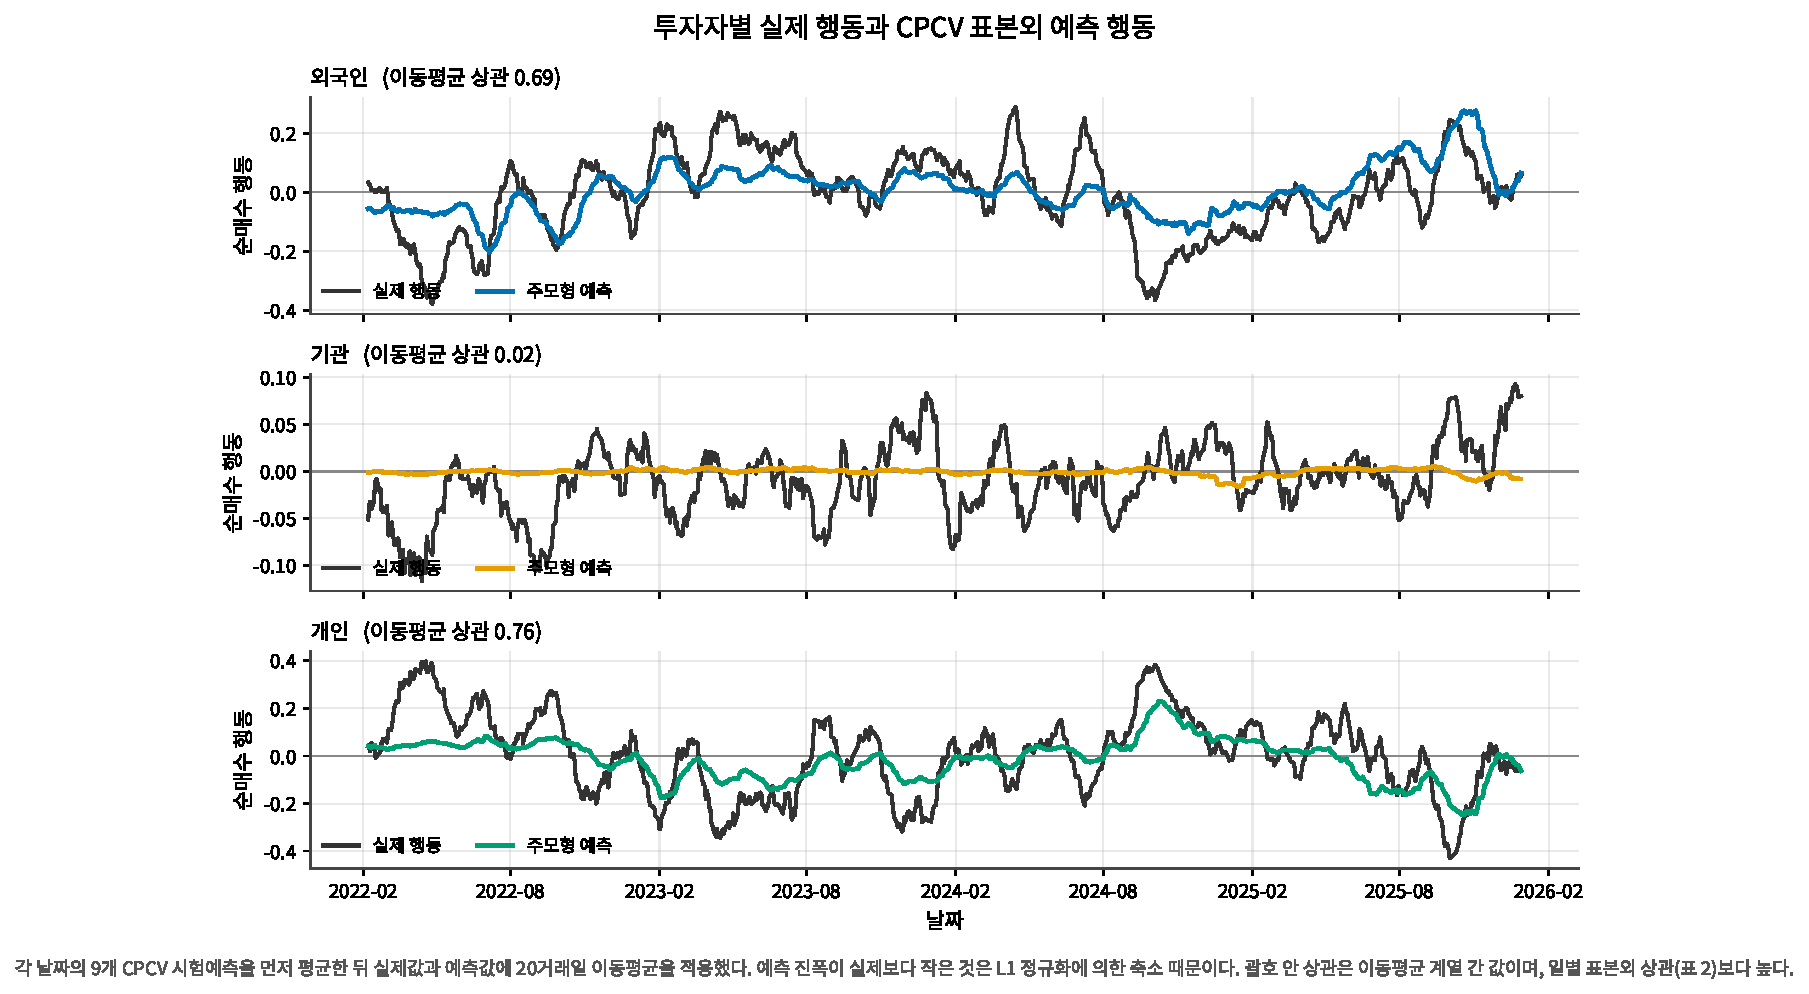
\includegraphics[width=\columnwidth]{../figures_v2/fig2_actual_vs_prediction.pdf}
  \caption{Actual and out-of-sample predicted net buying by investor type. The
  nine CPCV test predictions available for each date are averaged first, then a
  20-day moving average is applied to both the actual and the predicted series.
  Correlations in the panel titles are between the smoothed series and are not
  directly comparable to the daily out-of-sample correlations in
  Table~\ref{tab:performance}.}
  \Description{Three line charts overlaying actual net buying and model
  predictions over time for foreign, institutional and retail investors. In the
  institutional panel the prediction line is flat near zero.}
  \label{fig:prediction}
\end{figure}

Figure~\ref{fig:prediction} places actual and predicted net buying side by side
for the three types. Three things are immediately visible. First, for foreign
and retail investors the predicted series tracks the regime turns of the actual
series, with smoothed correlations of 0.69 and 0.76. Second, the predicted
amplitude is markedly smaller than the actual one, a consequence of coefficient
shrinkage under the $L_1$ penalty. Third, the institutional prediction is
essentially pinned to zero (0.02): the null reported in \S\ref{sec:null} appears
first in the prediction series rather than in a coefficient table.

\begin{table}[t]
  \caption{Out-of-sample performance under CPCV (mean $\pm$ s.d.\ over 45
  splits) and the persistence baseline}
  \label{tab:performance}
  \small
  \centering
  \begin{tabular}{@{}lccc@{}}
    \toprule
    Metric & Foreign & Institutional & Retail \\
    \midrule
    \multicolumn{4}{@{}l}{\emph{Main model}}\\
    Directional accuracy & $0.636\pm0.039$ & $0.542\pm0.038$ & $0.608\pm0.044$ \\
    Correlation          & $0.278\pm0.110$ & $0.068\pm0.064$ & $0.245\pm0.118$ \\
    MAE                  & $0.195\pm0.019$ & $0.094\pm0.008$ & $0.264\pm0.029$ \\
    RMSE                 & $0.246\pm0.021$ & $0.125\pm0.012$ & $0.318\pm0.030$ \\
    MAE / action s.d.    & $0.759$ & $0.756$ & $0.791$ \\
    Saturation rate      & $0.000$ & $0.000$ & $0.000$ \\
    \addlinespace
    \multicolumn{4}{@{}l}{\emph{Persistence baseline} ($a_{t+1}\leftarrow a_t$)}\\
    Directional accuracy & $\mathbf{0.642}$ & $\mathbf{0.547}$ & $\mathbf{0.616}$ \\
    Correlation          & $\mathbf{0.359}$ & $\mathbf{0.136}$ & $\mathbf{0.311}$ \\
    MAE                  & $0.223$ & $0.123$ & $0.299$ \\
    \addlinespace
    Action AR(1)         & $0.401$ & $0.149$ & $0.345$ \\
    \bottomrule
  \end{tabular}
\end{table}

\begin{figure}[t]
  \centering
  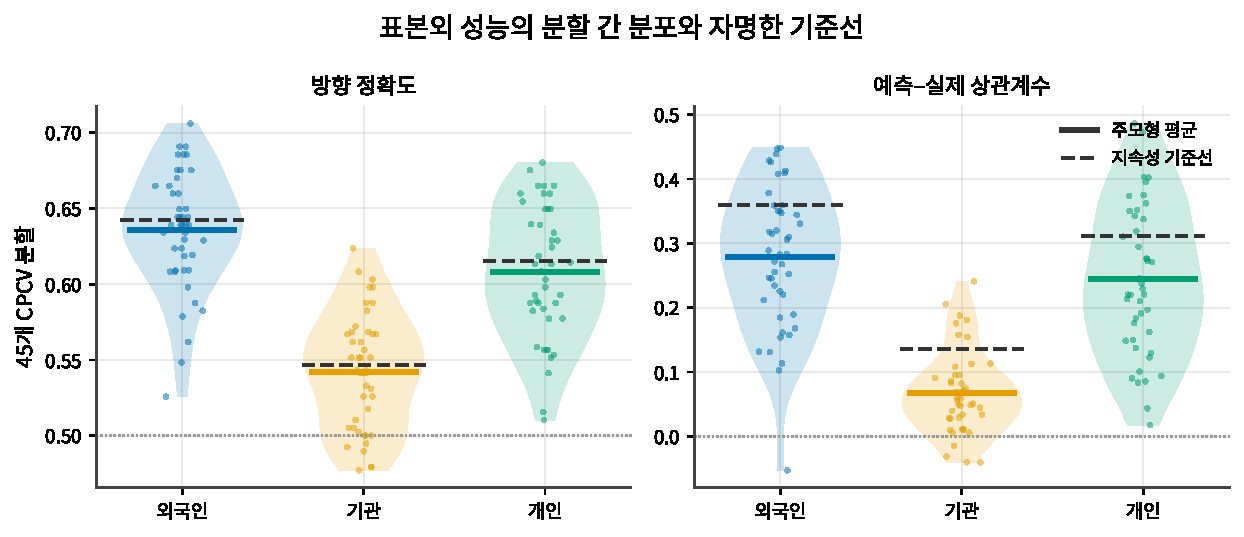
\includegraphics[width=\columnwidth]{../figures_v2/fig5_oos_performance.pdf}
  \caption{Split-level distribution of out-of-sample performance against a naive
  baseline. Solid lines are the main-model mean and dashed lines the persistence
  baseline. The dashed line lies above the solid line for all three types.}
  \Description{Two panels showing violin and point distributions of directional
  accuracy and correlation across 45 splits for the three investor types.}
  \label{fig:oos}
\end{figure}

Table~\ref{tab:performance} and Figure~\ref{fig:oos} reveal two things that
means alone conceal. First, dispersion across splits is large: the foreign
correlation ranges from $-0.05$ to $0.45$, so comparing types from a single
split is meaningless. Second, the naive persistence baseline outperforms the
main model on both directional accuracy and correlation. Since $a_t$ is
published after the day-$t$ close, this is an informationally feasible rule. The
main model leads only on MAE, and because that follows from shrinkage of the
predicted amplitude it cannot be read as an informational advantage.

The reason for the gap is clear. The action has first-order autocorrelation of
$0.401/0.149/0.345$, yet our reward feature set does not include the lagged own
action. Restricting the features to (F1)--(F3) was a design choice ensuring that
all three types share only features corresponding to independently established
behavioural regularities; it was not a design aimed at maximizing predictive
performance. We report this result openly in Table~\ref{tab:performance}.
Table~\ref{tab:performance} and Figure~\ref{fig:oos} are used to show that the
model has not merely fitted noise, not as evidence of predictive superiority.

Because the saturation rate is exactly zero for every type in every split, the
premise $|q|\le1$ of Proposition~\ref{prop:lasso} holds throughout the sample.
The estimator is therefore literally the Lasso of Equation~\eqref{eq:lasso}, and
performance does not rely on extreme $\pm1$ predictions.

\subsection{Recovered Rewards: A Mirror Image on the Momentum Axis}
\label{sec:beta}

\begin{figure*}[t]
  \centering
  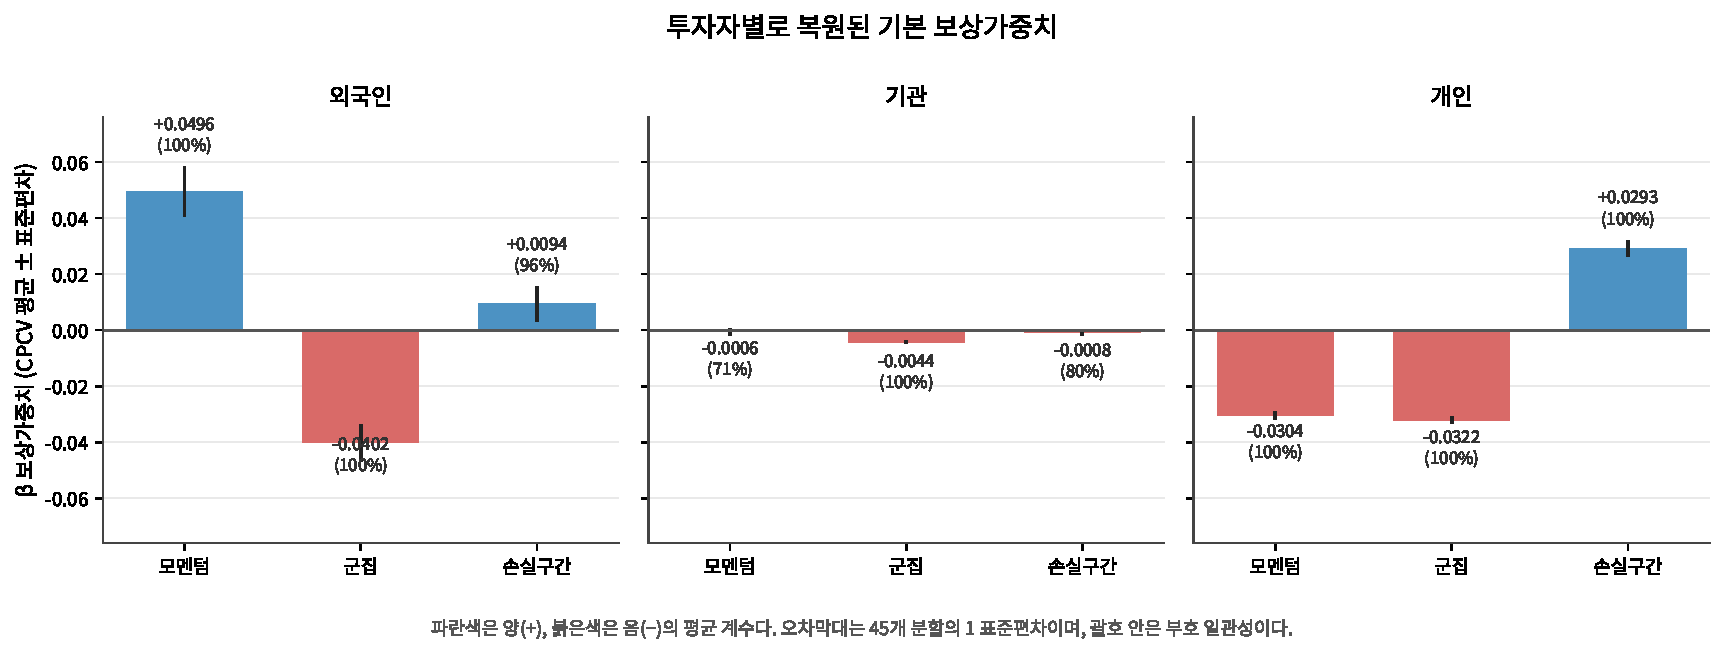
\includegraphics[width=\textwidth]{../figures_v2/fig1_reward_weights_bar.pdf}
  \caption{Recovered baseline reward weights $\beta$ by investor type. Blue bars
  are positive and red bars negative mean coefficients; error bars are one
  standard deviation across the 45 splits and the parenthesised figure is sign
  consistency.}
  \Description{Three bar charts giving momentum, herding and underwater
  coefficients for foreign, institutional and retail investors. Foreign momentum
  is positive, retail momentum negative, and the institutional bars are barely
  visible.}
  \label{fig:betabar}
\end{figure*}

\begin{figure*}[t]
  \centering
  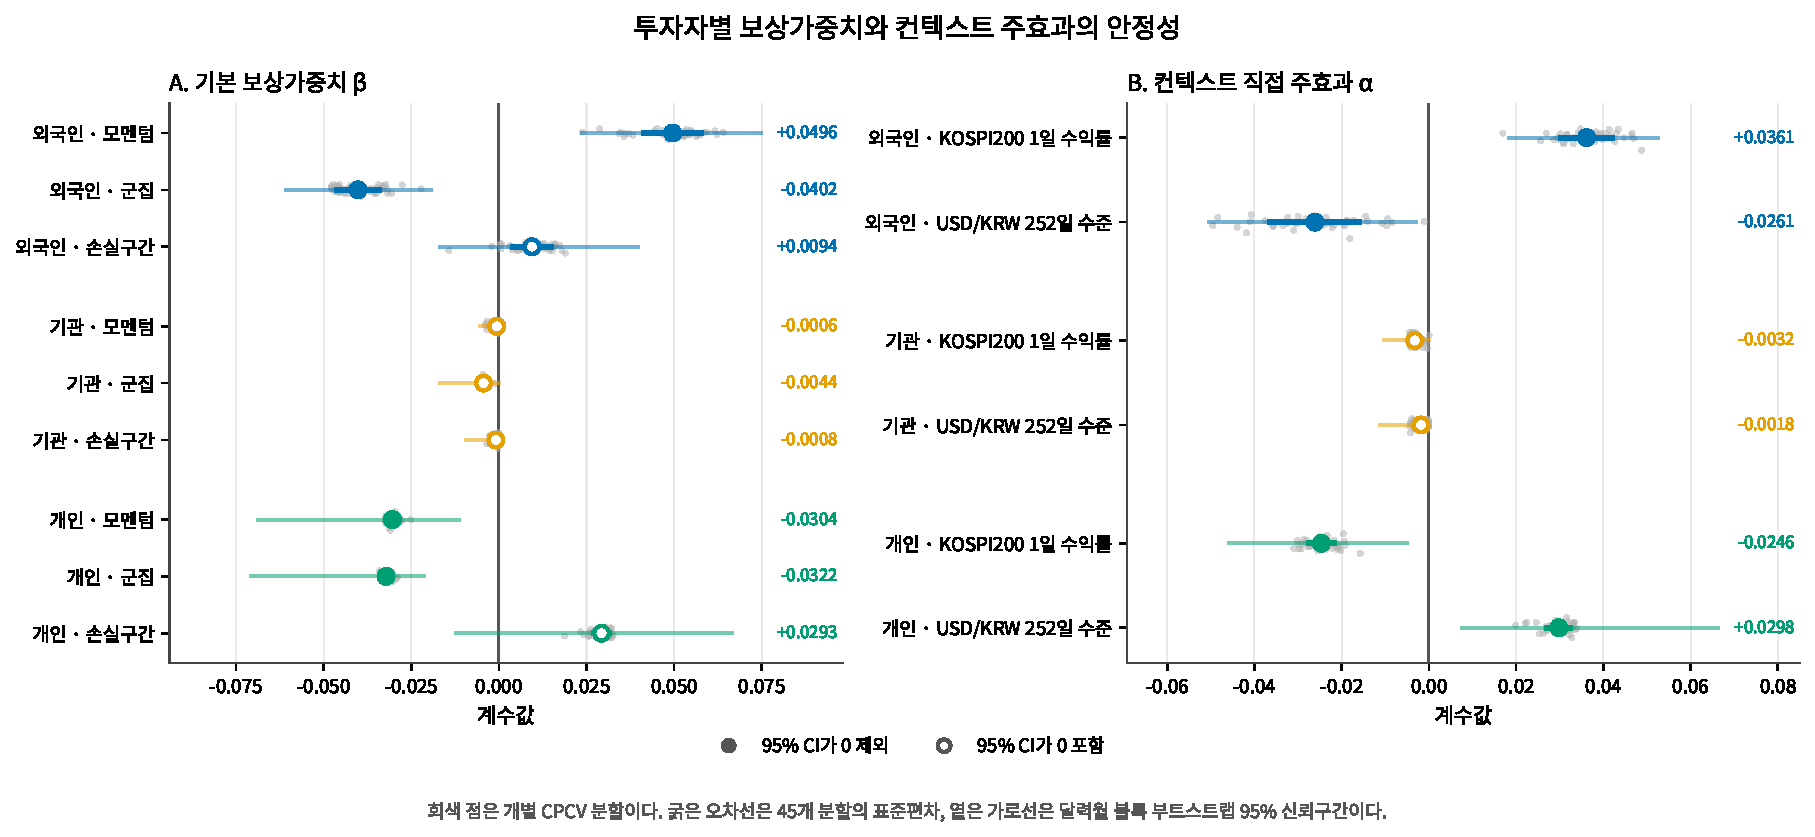
\includegraphics[width=\textwidth]{../figures_v2/fig3_beta_alpha_forest.pdf}
  \caption{Split-level stability of reward weights and context main effects.
  Grey dots are individual CPCV splits, thick error bars the standard deviation
  across the 45 splits, and light horizontal lines the 95\% calendar-month block
  bootstrap interval. Hollow markers denote terms whose interval contains zero.}
  \Description{Forest plots for baseline reward weights (panel A) and context
  main effects (panel B), showing per-split estimates and confidence intervals
  for each term.}
  \label{fig:forest}
\end{figure*}

Figure~\ref{fig:betabar} places the recovered baseline reward weights of the
three types side by side. Because all types received the same feature set and
the same model form and only their parameters were estimated separately, the
differences in bar height are entirely learned from the data.
Figure~\ref{fig:forest} unfolds the same $\beta$ together with the context main
effects $\alpha$ down to the split level.

\paragraph{The mirror image on the momentum axis}
The foreign momentum weight is $+0.0496$ and positive in all 45 splits, while
the retail weight is $-0.0304$ and negative in all 45 splits. In
Figure~\ref{fig:betabar} the two bars point in opposite directions across the
zero line, and in Figure~\ref{fig:forest} their bootstrap intervals do not
overlap and each excludes zero. Although the same feature set was estimated
independently for each type, the two types diverge in exactly opposite
directions on momentum: foreign investors appear as trend followers and retail
investors as contrarians, matching the sign expectations of prior
work~\cite{grinblatt2000investment,choe1999foreign}.

\paragraph{Herding}
The herding coefficient is negative in all 45 splits for all three types, and
the bootstrap intervals of the foreign ($-0.0402$) and retail ($-0.0322$)
coefficients also exclude zero. This result, however, does not separate a
behavioural interpretation from the market-clearing constraint. As
Figure~\ref{fig:crossinv} shows, the same-day correlation between types reaches
$-0.77$, so a substantial part of the negative herding coefficient may arise
mechanically. Because Equation~\eqref{eq:herd} uses a one-day lag the same-day
constraint does not apply directly, but it can propagate through the
autocorrelation of the action. We therefore restrict this result to the
descriptive statement that observed aggregate flow displays a negative
cross-type association, and do not extend it to the behavioural claim that each
type independently trades against the others.

\paragraph{Underwater}
The retail underwater weight is $+0.0293$ and positive in all 45 splits: buying
intensity rises on the following day when the traded price is below the
average-cost proxy, consistent with the reference-price dependence of the
disposition-effect literature~\cite{shefrin1985disposition,odean1998investors}.
The foreign coefficient shares the sign at $+0.0094$ (95.6\%) but is about a
third of the retail magnitude.

As Figure~\ref{fig:forest} shows, however, the underwater bootstrap interval
contains zero for all three types. The retail interval is
$[-0.0122,+0.0665]$: although the sign is 100\% consistent across the 45 splits,
it flips in 5.5\% of month-block resamples. This is exactly the situation
anticipated in \S\ref{sec:protocol}, where sign consistency understates
uncertainty because CPCV splits share observations. We therefore report that a
sign consistent with the disposition effect was observed, but do not claim it as
a statistically established result.

\subsection{Context Response: The Mirror Image Reappears}
\label{sec:alpha}

The mirror image observed on the momentum axis reappears in the context main
effects (panel B of Figure~\ref{fig:forest}). Foreign investors shift toward net
buying on days when the market rises ($+0.0361$) and toward net selling when the
won is weak ($-0.0261$), while retail investors do exactly the opposite on both
contexts ($-0.0246$ and $+0.0298$). All four coefficients keep their sign in all
45 splits and all four bootstrap intervals exclude zero. The two institutional
coefficients have sign consistency above 95\% but are about an eighth of the
foreign and retail magnitudes, and their intervals contain zero.

This mirror image requires the same interpretive reservation as the herding
coefficient. Given the $-0.772$ correlation in Figure~\ref{fig:crossinv}, two
types responding to context with opposite signs may in part reflect the
market-clearing constraint. We therefore present this as the descriptive fact
that the two types form opposite sides of order flow across market and exchange
rate conditions.

\paragraph{Interactions}
Of the twelve interaction coefficients, four keep their sign in all 45 splits:
foreign momentum $\times$ KOSPI200 ($-0.0139$), retail momentum $\times$ FX
($+0.0144$), retail herding $\times$ KOSPI200 ($-0.0080$) and retail
underwater $\times$ FX ($-0.0186$). Only the first and the last of these pass
the bootstrap. Since twelve coefficients were examined jointly, we present the
interactions as exploratory results only.

\subsection{Results of the Stability Protocol}
\label{sec:stability}

\paragraph{(V2) Calendar-month block bootstrap}
The light horizontal lines in Figure~\ref{fig:forest} give this result. The
bootstrap is a stricter criterion than CPCV sign consistency, and the outcome
splits three ways. First, the momentum mirror and the context mirror survive:
eight terms, comprising foreign and retail momentum, herding, and both context
main effects, all exclude zero. Second, the underwater weights do not survive.
Third, no institutional term excludes zero; all six institutional markers in
Figure~\ref{fig:forest} are hollow.

\begin{figure*}[t]
  \centering
  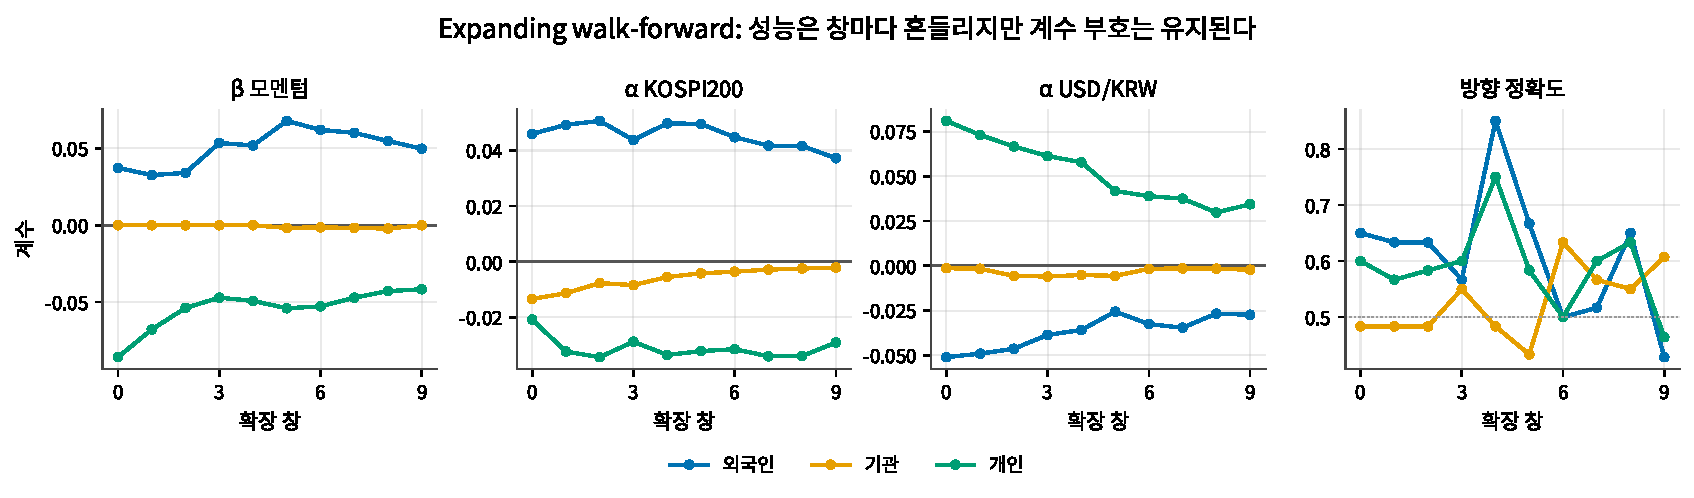
\includegraphics[width=\textwidth]{../figures_v2/fig6_walk_forward.pdf}
  \caption{Coefficient paths and directional accuracy over ten expanding
  walk-forward windows. Performance fluctuates from window to window while the
  coefficient signs hold.}
  \Description{Four line charts against the expanding-window index showing the
  momentum coefficient, the two context main effects, and directional accuracy
  for the three investor types.}
  \label{fig:walkforward}
\end{figure*}

\paragraph{(V3) Expanding walk-forward}
Figure~\ref{fig:walkforward} gives this result, and two things read at once.
Performance fluctuates sharply across windows: foreign directional accuracy
moves between 0.43 and 0.85, averaging $0.610\pm0.116$, and the correlation
falls to $0.131\pm0.162$, less than half the CPCV value of 0.278; retail falls
from 0.245 to 0.129. Because CPCV can place a test fold ahead of a training fold
while walk-forward cannot, we report this degradation as a generalization limit
arising from the temporal structure.

The coefficient paths, by contrast, do not fluctuate. The foreign momentum
coefficient is positive in all ten windows and the retail one negative in all
ten, and the two paths never cross. The same mirror image persists across all
windows for both context main effects, while the three institutional paths stay
pinned near zero. Performance moves with time; the direction of the recovered
preference does not.

\begin{figure*}[t]
  \centering
  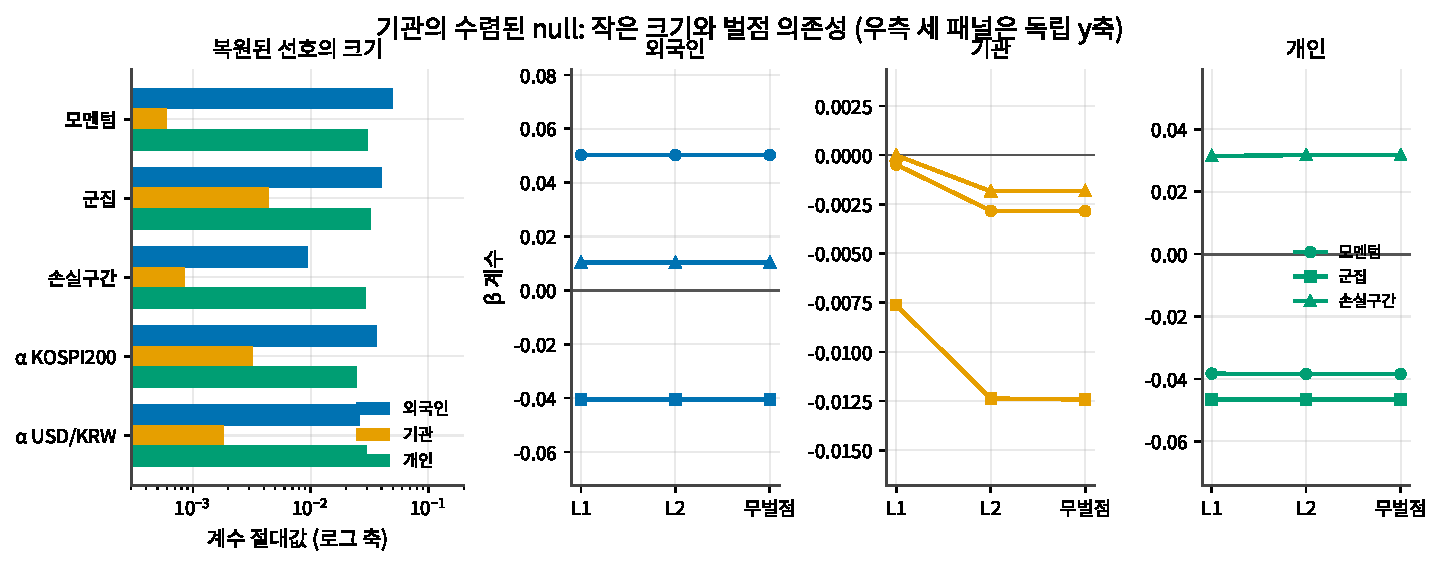
\includegraphics[width=\textwidth]{../figures_v2/fig7_institution_null.pdf}
  \caption{The converged institutional null. Left: magnitude of the recovered
  preferences on a logarithmic axis. Right: sensitivity to the regularization
  swap, with an independent $y$ axis in each of the three panels.}
  \Description{A logarithmic bar chart of coefficient magnitudes by type on the
  left, and three line charts of coefficients under L1, L2 and no penalty on the
  right.}
  \label{fig:null}
\end{figure*}

\paragraph{(V4) Regularization swap}
Figure~\ref{fig:null} gives this result. The foreign and retail coefficients are
effectively invariant to the choice of penalty, agreeing to four decimal places,
so the momentum mirror is not an artefact of the $L_1$ penalty. Only the
institutional coefficients move with the penalty (herding
$-0.0076\rightarrow-0.0124$, underwater $-0.0000\rightarrow-0.0018$), on a
$y$-axis range about one twentieth of that of the other two types. That the
coefficients depend on the choice of penalty means the data do not determine
their value.

\subsection{Institutional Investors: A Converged Null}
\label{sec:null}

For institutional order flow we find no preference that is stably identified at
daily frequency, and we report this as a finding rather than concealing it. The
evidence is fivefold and all of it is visible in the figures.

\begin{enumerate}
\item \textbf{Degenerate prediction.} In the middle panel of
Figure~\ref{fig:prediction} the institutional prediction stays on the zero line
while the actual series moves between $\pm0.1$.
\item \textbf{Magnitude.} In Figure~\ref{fig:betabar} the three institutional
bars are barely visible on the shared axis. Excluding herding, momentum is
$-0.0006$ and underwater $-0.0008$, about one fortieth of the other types.
\item \textbf{Uncertainty.} All six institutional markers in
Figure~\ref{fig:forest} are hollow.
\item \textbf{Penalty dependence.} In the middle right panel of
Figure~\ref{fig:null}, only the institutional coefficients move with the
penalty.
\item \textbf{Temporal instability.} In Figure~\ref{fig:walkforward} the
institutional paths hug the zero line; momentum sign consistency is 40\% of ten
windows and underwater 0\%.
\end{enumerate}

\begin{figure*}[t]
  \centering
  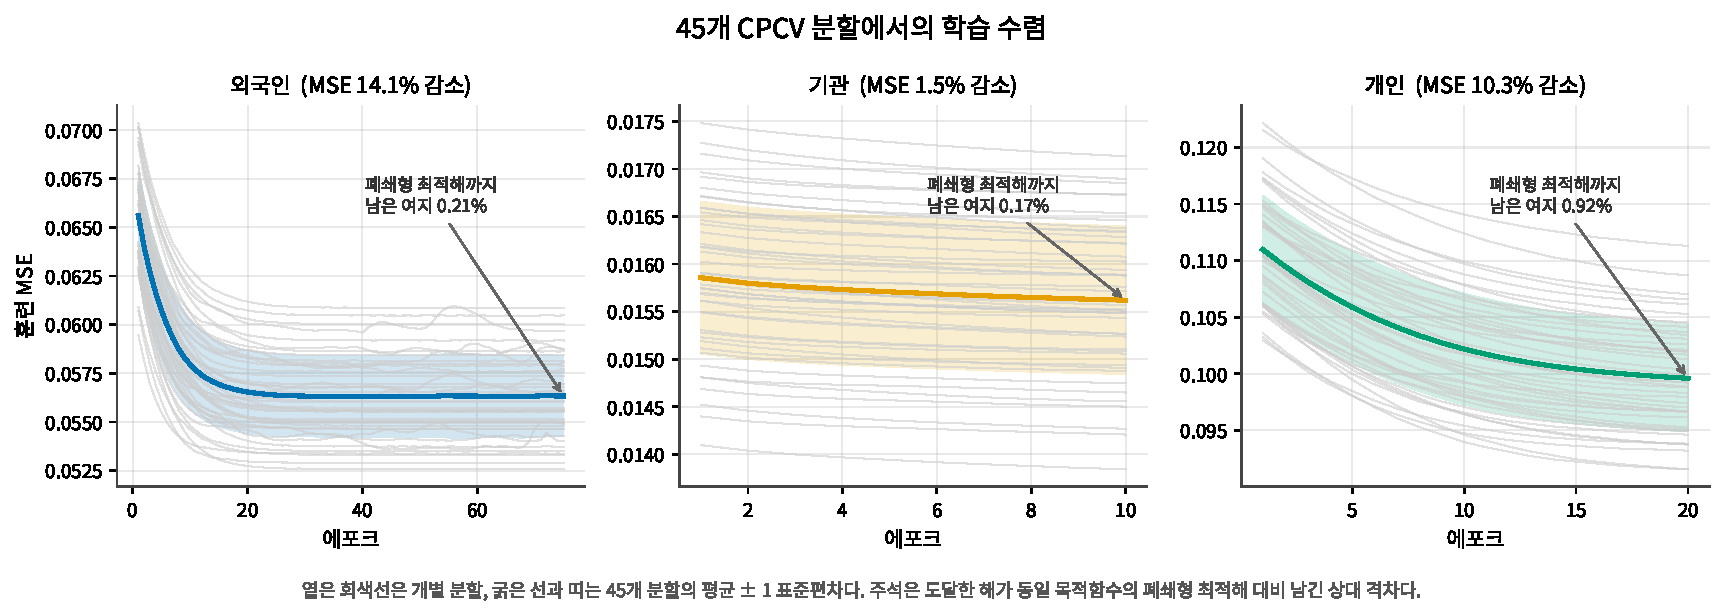
\includegraphics[width=\textwidth]{../figures_v2/fig4_training_convergence.pdf}
  \caption{Training convergence across the 45 CPCV splits. Light grey lines are
  individual splits; the thick line and band are the mean $\pm$ one standard
  deviation. The annotation gives the relative gap between the solution reached
  and the closed-form optimum of the same objective.}
  \Description{Three panels of training MSE against epoch for the three investor
  types; the institutional panel shows the smallest decrease.}
  \label{fig:convergence}
\end{figure*}

This null is not an optimization failure. Figure~\ref{fig:convergence} shows the
training curves across the 45 splits. The institutional training MSE falls by
only 1.5\% over the whole training run and the curve does not look visually
flat. That is not underfitting, however, but the fact that there is almost no
error left to remove. By Proposition~\ref{prop:lasso}, Equation~\eqref{eq:loss}
is convex with a unique global optimum, and comparing the solution reached with
the closed-form optimum of the same objective leaves an institutional gap of
only 0.17\% on average and 0.48\% at most (0.21\% for foreign and 0.92\% for
retail). All three types reach the attainable optimum; only for institutional
investors do the coefficients at that optimum sit near zero. The data do not
determine an institutional preference; it is not that the optimizer failed to
find one.

Economically the null reads naturally. The ``institutional'' category aggregates
pension funds, investment trusts, insurers, private funds, and securities firms,
so the flows of agents with different objective functions offset one another.
The one consistently negative herding coefficient is compatible with a shared
liquidity-provision role on the opposite side of the other types, but because
its bootstrap interval sits on the boundary we do not claim it.

\subsection{Construct Validity Check}
\label{sec:construct}

\begin{table}[t]
  \caption{Prior sign expectations and recovered results}
  \label{tab:construct}
  \small
  \begin{tabular}{@{}>{\raggedright\arraybackslash}p{0.26\columnwidth}
                  >{\raggedright\arraybackslash}p{0.14\columnwidth}
                  >{\raggedright\arraybackslash}p{0.24\columnwidth}
                  >{\raggedright\arraybackslash}p{0.20\columnwidth}@{}}
    \toprule
    Regularity & Expected & Recovered & Verdict \\
    \midrule
    Foreign trend trading~\cite{grinblatt2000investment,choe1999foreign}
      & $\beta^{mom}>0$ & $+0.0496$ (100\%, CI excl.\ 0) & matches \\
    Retail contrarian trading~\cite{grinblatt2000investment,kaniel2008individual}
      & $\beta^{mom}<0$ & $-0.0304$ (100\%, CI excl.\ 0) & matches \\
    Disposition effect~\cite{shefrin1985disposition,odean1998investors}
      & $\beta^{uw}>0$ & $+0.0293$ (100\%, CI incl.\ 0) & partial \\
    Institutional herding~\cite{lakonishok1992impact}
      & $\beta^{herd}>0$ & $-0.0044$ (100\%, CI incl.\ 0) & mismatch \\
    \bottomrule
  \end{tabular}
\end{table}

Table~\ref{tab:construct} reports the contrast. Although all three types
received the same features and the same model form and only their parameters
were estimated separately, the recovered signs agree with independently
established regularities and the two types diverge in opposite directions on
momentum. This is evidence of construct validity: the recovered reward is not an
arbitrary fit.

The mismatch arises because the measured object differs. Lakonishok et
al.~\cite{lakonishok1992impact} measure the extent to which agents \emph{within}
the institutional group move in the same direction, whereas
Equation~\eqref{eq:herd} measures whether institutions move with the previous
day's flow of the \emph{other two types}. Our result is therefore not a
refutation of that literature; testing within-type herding would require data on
institutional sub-categories.

\subsection{What This Study Does Not Claim}
\label{sec:notclaim}

As the final stage of the protocol we state explicitly what the results do not
support.

\begin{enumerate}
\item \textbf{Return predictability.} Our metrics are reproduction errors for
the direction and intensity of order flow and include no returns, Sharpe ratios,
or transaction costs. No trading rule follows from
Table~\ref{tab:performance}.

\item \textbf{Superior flow prediction.} As reported in
Table~\ref{tab:performance} and Figure~\ref{fig:oos}, the persistence baseline
beats the main model on directional accuracy and correlation. Our objective is
preference recovery on an interpretable common scale rather than predictive
performance, and the two objectives call for different feature sets. In a
preliminary check, adding the lagged own action as a fourth feature lifts the
model above the baseline (directional accuracy $0.646/0.569/0.629$) but reverses
the sign of the retail $\alpha^{KOSPI}$ and eliminates the underwater
coefficient. Some of the mirror images reported here are therefore not separable
from the autocorrelation of order flow.

\item \textbf{Causal effects.} The recovered weights are conditional
associations among standardized observed features. Because feature--context
correlations range from $-0.29$ to $0.22$ (Figure~\ref{fig:featcorr}), the
magnitude of any coefficient depends on the other terms being controlled for.

\item \textbf{A behavioural reading of the negative cross-type association.} The
herding coefficient and the mirrored context responses are not separable from
the market-clearing constraint (Figure~\ref{fig:crossinv}).

\item \textbf{A test of the disposition effect.} The retail underwater sign
agrees with the literature but does not pass the month-block bootstrap
(Figure~\ref{fig:forest}), and the average-cost proxy is built from aggregate
trades rather than account-level realized gains and holding periods.

\item \textbf{Generalization across stocks.} The single-stock design is a
control for isolating heterogeneity across types; extension to other stocks and
markets is untested.
\end{enumerate}

% =====================================================================
\appendix

\section{Supplementary Material}
\label{sec:appendix}

This appendix collects the supporting figures and tables referenced in the main
text. Figure~\ref{fig:saturation} verifies the premise of
Proposition~\ref{prop:lasso}, Figure~\ref{fig:featcorr} reports
feature--context correlations, and Figure~\ref{fig:crossinv} shows same-day
actions across types. Table~\ref{tab:interactions} lists the full set of
interaction coefficients presented as exploratory in the main text, and
Table~\ref{tab:convergence} reports the optimality check of the solution
reached.

\begin{figure}[htbp]
  \centering
  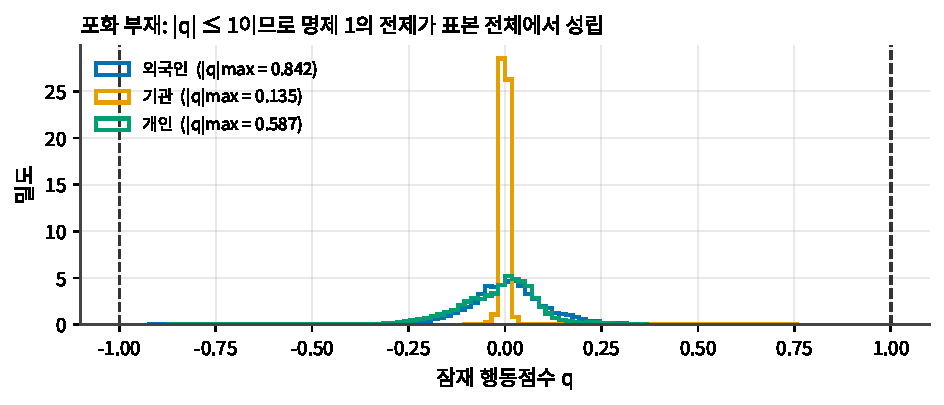
\includegraphics[width=\columnwidth]{../figures_v2/figA1_no_saturation.pdf}
  \caption{Distribution of the latent action score against the action bounds.
  Since $|q|\le1$, the premise of Proposition~\ref{prop:lasso} holds throughout
  the sample and the saturation rate is exactly zero in all 45 splits.}
  \Description{Histograms of the latent action score for the three types with
  the $\pm1$ bounds marked.}
  \label{fig:saturation}
\end{figure}

\begin{figure}[htbp]
  \centering
  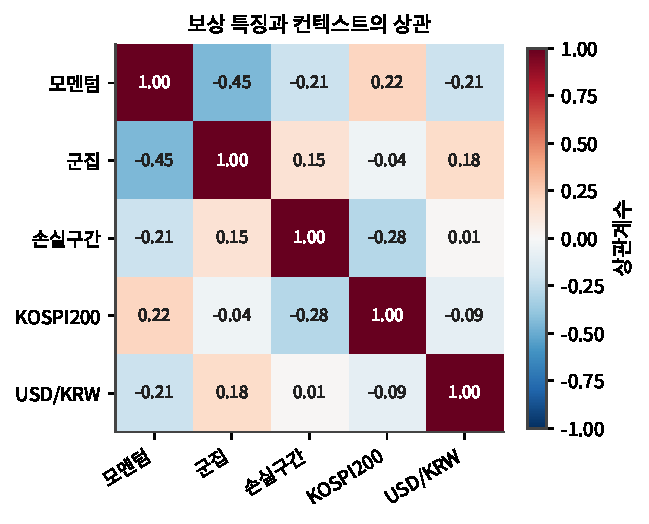
\includegraphics[width=\columnwidth]{../figures_v2/figA2_feature_correlation.pdf}
  \caption{Correlation matrix of reward features and contexts (foreign features,
  973 observations).}
  \Description{A heatmap showing correlation coefficients among five variables
  in colour and numerals.}
  \label{fig:featcorr}
\end{figure}

\begin{figure}[htbp]
  \centering
  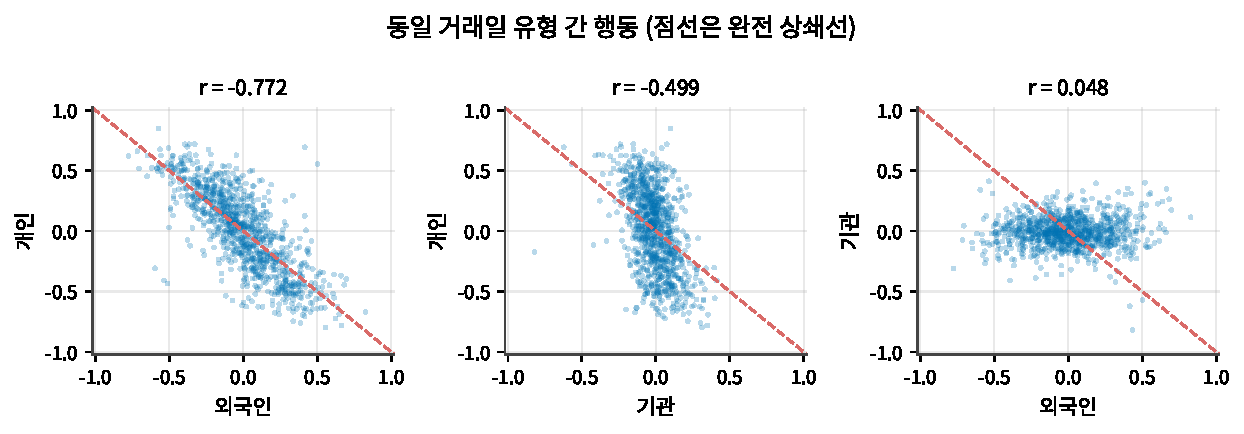
\includegraphics[width=\columnwidth]{../figures_v2/figA3_cross_investor_actions.pdf}
  \caption{Same-day actions across investor types. The dashed line marks perfect
  offset; foreign and retail actions cluster along it.}
  \Description{Three scatter plots of actions for each pair of investor types
  with the corresponding correlation coefficients.}
  \label{fig:crossinv}
\end{figure}

\begin{table}[htbp]
  \caption{Interaction coefficients $B$ (45 splits)}
  \label{tab:interactions}
  \small
  \centering
  \begin{tabular}{@{}llrrr@{}}
    \toprule
    Type & Feature $\times$ context & Mean & S.d. & Sign cons. \\
    \midrule
    Foreign & momentum $\times$ KOSPI200 & $-0.0139$ & $0.0052$ & 100.0\% \\
    Foreign & momentum $\times$ FX       & $-0.0030$ & $0.0057$ & 71.1\% \\
    Foreign & herding $\times$ KOSPI200  & $+0.0016$ & $0.0074$ & 66.7\% \\
    Foreign & herding $\times$ FX        & $+0.0037$ & $0.0073$ & 68.9\% \\
    Foreign & underwater $\times$ KOSPI200 & $-0.0062$ & $0.0040$ & 93.3\% \\
    Foreign & underwater $\times$ FX     & $-0.0075$ & $0.0076$ & 86.7\% \\
    \addlinespace
    Inst. & momentum $\times$ KOSPI200 & $-0.0001$ & $0.0005$ & 66.7\% \\
    Inst. & momentum $\times$ FX       & $+0.0003$ & $0.0006$ & 80.0\% \\
    Inst. & herding $\times$ KOSPI200  & $-0.0004$ & $0.0006$ & 86.7\% \\
    Inst. & herding $\times$ FX        & $+0.0012$ & $0.0012$ & 93.3\% \\
    Inst. & underwater $\times$ KOSPI200 & $+0.0028$ & $0.0012$ & 97.8\% \\
    Inst. & underwater $\times$ FX     & $+0.0007$ & $0.0008$ & 91.1\% \\
    \addlinespace
    Retail & momentum $\times$ KOSPI200 & $+0.0021$ & $0.0042$ & 80.0\% \\
    Retail & momentum $\times$ FX       & $+0.0144$ & $0.0045$ & 100.0\% \\
    Retail & herding $\times$ KOSPI200  & $-0.0080$ & $0.0046$ & 100.0\% \\
    Retail & herding $\times$ FX        & $+0.0092$ & $0.0081$ & 82.2\% \\
    Retail & underwater $\times$ KOSPI200 & $-0.0022$ & $0.0046$ & 66.7\% \\
    Retail & underwater $\times$ FX     & $-0.0186$ & $0.0046$ & 100.0\% \\
    \bottomrule
  \end{tabular}
\end{table}

\begin{table}[htbp]
  \caption{Optimality check of the solution reached (45 splits)}
  \label{tab:convergence}
  \small
  \centering
  \begin{tabular}{@{}lccc@{}}
    \toprule
    Type & MSE drop & Gap (\%) & Cosine \\
     & (training) & mean / max & mean / min \\
    \midrule
    Foreign & 14.1\% & $0.21/3.10$ & $0.994/0.948$ \\
    Inst.   & 1.5\%  & $0.17/0.48$ & $0.935/0.832$ \\
    Retail  & 10.3\% & $0.92/1.40$ & $0.894/0.833$ \\
    \bottomrule
  \end{tabular}
\end{table}

%  Required packages: booktabs, graphicx, amsmath, array, url
%  Figure path: ../figures_v2/  (output of scripts/make_paper_figures.py)
%  Additional references: merge paper-refs-additional.bib
% =====================================================================

\section{Method}
\label{sec:method}

\subsection{Setup: Symmetric Estimation}
\label{sec:setup}

Let the set of investor types be
$\mathcal{I}=\{\text{foreign},\text{institutional},\text{retail}\}$. Each type is
treated as an agent whose observed daily order flow reveals a latent reward
defined over interpretable market state features.

\paragraph{Continuous action}
Writing $V^{buy}_{i,t}$ and $V^{sell}_{i,t}$ for the daily gross buy and gross
sell value of type $i$, we define the action as
\begin{equation}
u_{i,t}=\frac{V^{buy}_{i,t}-V^{sell}_{i,t}}
             {V^{buy}_{i,t}+V^{sell}_{i,t}}\in[-1,1].
\label{eq:action}
\end{equation}
Because the denominator is the type's own gross turnover rather than
market-wide turnover, $u_{i,t}$ measures whether buying or selling dominated
\emph{within} that type, giving a common scale that is unaffected by
differences in trading size across types. Using a continuous intensity rather
than a binary buy/sell label preserves the magnitude information that
dichotomization discards.

\paragraph{Symmetry}
All three types receive the same state features $x_{i,t}\in\mathbb{R}^{3}$, the
same market context $C_t\in\mathbb{R}^{2}$, and the same model form. No type is
assigned a different feature a priori; only the parameters
$\theta_i=(\beta_i,B_i,\alpha_i)$ are estimated separately on each type's own
data. Any difference that appears in the results is therefore learned from the
data rather than imposed by design, and this symmetry is what licenses direct
comparison of coefficients across types.

\paragraph{Timing}
The training sample is $(x_{i,t},C_t,a_{i,t+1})$ with $a_{i,t+1}=u_{i,t+1}$. A
state built from day-$t$ closing prices and order flow explains day-$t+1$
behaviour, so no future trade enters the features. Momentum and underwater use
day-$t$ information while the herding feature uses day $t-1$. Since the target
is day-$t+1$ behaviour, day-$t$ information is also available; the extra lag on
herding is therefore not an information constraint but a design choice that
keeps the same-day accounting offset between types out of the predictor set
(Figure~\ref{fig:crossinv}).

\subsection{Reward Features}
\label{sec:features}

All three features are standardized using statistics fitted on the training
indices of each validation split only. Every coefficient reported below is
therefore read as the effect of a one-standard-deviation move of that feature
within the training window.

\paragraph{(F1) Medium-term momentum}
With adjusted (or fallback) closing price $P_t$,
\begin{equation}
x^{mom}_{i,t}=\log\!\left(\frac{P_t}{P_{t-20}}\right).
\label{eq:momentum}
\end{equation}
Twenty trading days is a pre-specified window of roughly one month, chosen to
damp daily price noise while still expressing a medium-term trend linked to
next-day behaviour. It is a design value for interpretability, not a value tuned
on the data. A positive coefficient indicates trend following and a negative one
contrarian trading; the sign expectation follows prior work on type-specific
momentum trading~\cite{grinblatt2000investment,choe1999foreign}.

\paragraph{(F2) Herding}
The cross-sectional average of the previous day's actions of the two types other
than $i$:
\begin{equation}
x^{herd}_{i,t}=\frac{u_{j,t-1}+u_{k,t-1}}{2},\qquad j,k\neq i.
\label{eq:herd}
\end{equation}
Note that this is an average across the two other types at one point in time,
not a time average. A 20-day moving average would measure a month of cumulative
flow pressure rather than an immediate response, so we focus on the previous
day. A positive coefficient means moving with the previous day's direction of
the other types, a negative one means moving against it. The sign expectation
follows the institutional herding
literature~\cite{lakonishok1992impact}; note however that this literature
measures herding \emph{within} the institutional group, whereas
Equation~\eqref{eq:herd} measures a relation \emph{between} types
(\S\ref{sec:construct}).

\paragraph{(F3) Underwater gap relative to average cost}
With a per-type average-cost proxy $\bar P_{i,t}$ and the day's gross-trade VWAP
$P^{vwap}_{i,t}$,
\begin{equation}
x^{uw}_{i,t}=\max\!\left(
\frac{\bar P_{i,t}-P^{vwap}_{i,t}}{\bar P_{i,t}},\,0\right).
\label{eq:underwater}
\end{equation}
Truncation at zero makes the feature active only when the traded price sits
below the average-cost proxy, so the variable is reference-point dependent by
construction. The average cost is obtained by recursively updating an effective
inventory from gross buy and sell quantities and values: the previous day's
inventory is multiplied by a forgetting factor $\rho=0.98$ to damp the influence
of old trades, and sales do not change the average cost of the remaining
position. With $\rho=0.98$ the half-life is about 34 trading days and roughly
66.8\% remains after 20, so the feature emphasises the trading memory of the
past one to two months; this value was also not tuned on the data. A positive
coefficient means stronger next-day buying below the average cost, and the sign
expectation follows the disposition-effect
literature~\cite{shefrin1985disposition,odean1998investors}.

The proxy is constructed from aggregate flow rather than actual account
holdings. Buys and sells executed by different accounts within the same type
net out, so the notion of a ``representative investor's average cost'' is itself
an approximation. The coefficient on $x^{uw}$ therefore cannot be read as a
direct test of the disposition effect.

\subsection{Market Context}
\label{sec:context}

The context consists of two variables: (C1) the one-day KOSPI200 return $r_t$,
and (C2) the KRW/USD exchange rate level
\begin{equation}
z_t=\frac{\log e_t-\mu_{t-1,252}}{\sigma_{t-1,252}},
\label{eq:fxcontext}
\end{equation}
where the current rate is used but the mean and standard deviation are computed
only through $t-1$ over 252 trading days. Both contexts are likewise
re-standardized on the training indices of each split, so their coefficients
read as the effect of a one-standard-deviation move within the training window.

Context and reward features are not independent. Because Samsung Electronics
carries a large weight in the KOSPI200, stock momentum overlaps with the market
return, and feature--context correlations range from $-0.29$ to $0.22$
(Figure~\ref{fig:featcorr}). Individual coefficients are therefore conditional
associations given the other terms and should not be read as causal magnitudes
in isolation.

\subsection{Myopic Reward, Policy, and the Reduction to Lasso}
\label{sec:model}

\paragraph{Latent action score}
Define the action score of type $i$ at time $t$ as
\begin{equation}
q_{i,t}=(\beta_i+B_iC_t)^{\top}x_{i,t}+\alpha_i^{\top}C_t,
\label{eq:score}
\end{equation}
where $\beta_i\in\mathbb{R}^{3}$ is the baseline reward weight at average
context, $B_i\in\mathbb{R}^{3\times 2}$ the feature--context interaction, and
$\alpha_i\in\mathbb{R}^{2}$ the direct context main effect. The $\alpha$ term is
a level effect that shifts behaviour even when the stock features are at their
means; the $B$ term is a slope effect that changes sensitivity to each feature
across market conditions. Including interaction terms while omitting the
lower-order term $C_t$ is a standard specification error, so the inclusion of
$\alpha$ is required by the specification rather than something to be justified
empirically.

\paragraph{Myopic concave reward}
The one-step reward for a continuous action $a$ is
\begin{equation}
R_i(x,C,a)=q_{i,t}\,a-\frac{\kappa}{2}a^{2}.
\label{eq:reward}
\end{equation}
The quadratic term imposes a symmetric cost on large net buying and net selling
and makes the reward concave in the action, which permits an interior solution.
Without it, maximizing over $[-1,1]$ would return $\pm1$ almost always depending
only on the sign of $q$, and the \emph{intensity} of behaviour could not be
reproduced. Maximizing Equation~\eqref{eq:reward} over $a$ yields the closed-form
policy
\begin{equation}
a^{*}_{i,t+1}=\mathrm{clip}\!\left(\frac{q_{i,t}}{\kappa},-1,1\right).
\label{eq:policy}
\end{equation}
The curvature $\kappa$ is fixed at one for identification. With $\kappa=2$ the
same $q$ would halve the action size, but re-estimation would double the
coefficients of $q$ and reproduce the same behaviour; $\kappa=1$ therefore fixes
the units of the reward and the coefficients rather than asserting that the
empirical curvature equals one.

\paragraph{Estimation}
The training objective for each type on its training set $\mathcal{D}_i$ is
\begin{equation}
\min_{\theta_i}\ \frac{1}{|\mathcal{D}_i|}
\sum_{t\in\mathcal{D}_i}\bigl(a^{*}_{i,t+1}-a_{i,t+1}\bigr)^{2}
+\lambda_i\lVert\theta_i\rVert_1,
\label{eq:loss}
\end{equation}
optimized independently per type with Adam~\cite{kingma2015adam}.

\begin{proposition}[Reduction to Lasso]
\label{prop:lasso}
Let
$z_{i,t}=[\,x_{i,t};\ \mathrm{vec}(x_{i,t}C_t^{\top});\ C_t\,]\in\mathbb{R}^{11}$
and $\theta_i=[\,\beta_i;\ \mathrm{vec}(B_i);\ \alpha_i\,]$, so that
Equation~\eqref{eq:score} reads $q_{i,t}=\theta_i^{\top}z_{i,t}$. If
$|q_{i,t}|\le 1$ throughout the training sample, the clip in
Equation~\eqref{eq:policy} never binds, $a^{*}=q$, and
Equation~\eqref{eq:loss} becomes
\begin{equation}
\min_{\theta_i}\ \frac{1}{|\mathcal{D}_i|}
\sum_{t}\bigl(\theta_i^{\top}z_{i,t}-a_{i,t+1}\bigr)^{2}
+\lambda_i\lVert\theta_i\rVert_1,
\label{eq:lasso}
\end{equation}
which is exactly an $L_1$-penalized (Lasso) regression of next-day net-buying
intensity on the expanded state feature $z$.
\end{proposition}

Under a myopic concave reward with $\kappa=1$, ``recovering a preference'' and
``regressing order flow'' are therefore numerically indistinguishable.
Figure~\ref{fig:saturation} shows that the premise of
Proposition~\ref{prop:lasso} in fact holds in our sample: for all three types the
distribution of the latent action score sits far inside the action bounds
$\pm1$ (the maximum $|q|$ is 0.842 for foreign, 0.587 for retail and 0.135 for
institutional investors), and the saturation rate is exactly zero in all 45
splits.

\paragraph{Why we do not hide the reduction}
This coincidence is not a weakness of the method but a logical consequence of
the myopia assumption. If the agent looks only one step ahead, today's action
does not affect anything beyond tomorrow, so there is no future to look toward
and \emph{what the agent wants} (the reward) collapses onto \emph{what the agent
does} (the policy). Applying the stochastic policy of maximum-entropy
IRL~\cite{ziebart2008maximum}, $\pi(a\mid x,C)\propto\exp(R/\tau)$, to
Equation~\eqref{eq:reward} makes $\pi$ a truncated normal with mean $q$ and
variance $\tau$, whose maximum-likelihood point estimate coincides with
Equation~\eqref{eq:lasso}. The reduction is thus a property of the myopic,
quadratic-reward setting in general, not an artefact of one implementation.

The distinctive value of the inverse reinforcement learning formulation lies in
the extension path. Once state dynamics and multi-period value are introduced,
the reward separates from the policy and leads to a structural recovery that
regression cannot reach. This paper is the first step on that path, and it adds
interpretation and validation on top of an explicitly stated set of conditions.

\subsection{Validation Protocol}
\label{sec:protocol}

Rather than stopping at the sign and magnitude of the recovered coefficients, we
apply four stages.

\begin{description}
\item[(V1) Out-of-sample stability under CPCV] We use combinatorial purged
cross-validation~\cite{lopez2018advances} with ten temporal folds of which two
serve as test folds, giving $\binom{10}{2}=45$ splits, a one-day purge and a
five-day embargo between training and test, and all standardization fitted on
training indices only. We report the fraction of splits in which the dominant
sign appears (sign consistency), but because the splits share observations we
interpret sign consistency only as a stability indicator, never as an
independent-sample $p$-value.

\item[(V2) Calendar-month block bootstrap] To address the fact that sign
consistency is not a test, we partition the sample into calendar-month blocks,
resample months with replacement, and re-estimate 1{,}000 times to obtain 95\%
confidence intervals. Month blocks preserve the autocorrelation of daily flow
and within-month patterns inside each block.

\item[(V3) Expanding walk-forward] Because CPCV can place a test fold before a
training fold, we add a validation that strictly respects the arrow of time. We
train on the first 400 observations, predict the next 60 trading days after a
five-day purge, and repeat while expanding the training window by 60 trading
days, for ten windows in total.

\item[(V4) Regularization swap] To confirm that the results are not an artefact
of the $L_1$ penalty, we re-run the same protocol with an $L_2$ penalty and with
no penalty, and compare coefficient signs.
\end{description}

\paragraph{Metrics}
Magnitude error is measured by MAE and RMSE, and directional reproduction by
directional accuracy, the fraction of days with
$\mathrm{sign}(a^{*})=\mathrm{sign}(a)$. We also report the Pearson correlation
between actual and predicted actions and the saturation rate, the fraction with
$|a^{*}|=1$. Because action standard deviations differ across types, absolute
MAE and RMSE are not compared across types but interpreted within each type, and
we report errors normalized by the action standard deviation alongside them. As
a reference we also report a persistence rule that predicts the previous day's
own action (\S\ref{sec:notclaim}).

\paragraph{Construct validity check}
We contrast the recovered signs with expectations derived from independently
established behavioural-finance regularities (\S\ref{sec:construct}). This is a
comparison against sign expectations fixed in advance, not a post hoc
interpretation.

% =====================================================================
\section{Experiments}
\label{sec:experiments}

\subsection{Data and Setup}
\label{sec:data}

The raw data are daily records for Samsung Electronics (005930) and include
prices, trading value, gross buy and sell values and quantities by investor
type, the KRW/USD exchange rate, and KOSPI200 returns. Among the observations
for which the 252-day exchange-rate history, the 20-day momentum, and the next
day's action can all be computed, we use the most recent 973 rows. State dates
run from 6 January 2022 to 29 December 2025, with the last state targeting the
action of 30 December 2025.

The single-stock design is not a limitation of the sample but a controlled
demonstration setting that isolates preference heterogeneity across types
without cross-stock confounding. Because stock fixed effects, liquidity
differences, and index-inclusion effects do not intervene, differences in
coefficients across types can be attributed to learning rather than design.

\begin{table}[t]
  \caption{Data and estimation setup}
  \label{tab:setup}
  \small
  \begin{tabular}{@{}>{\raggedright\arraybackslash}p{0.30\columnwidth}
                  >{\raggedright\arraybackslash}p{0.62\columnwidth}@{}}
    \toprule
    Item & Setting \\
    \midrule
    Sample & 973 trading days, 2022-01-06--2025-12-29 \\
    Types & foreign, institutional, retail (symmetric estimation) \\
    Reward features & momentum (20d), herding (1d lag), underwater ($\rho=0.98$) \\
    Contexts & KOSPI200 1d return, USD/KRW 252d level $z$ \\
    Parameters per type & 11 ($\beta$ 3, $B$ 6, $\alpha$ 2) \\
    Common settings & seed 42, CPU, $\kappa=1$, train-only scaling \\
    Foreign & 75 epochs, batch 256, lr 0.001, $\lambda=0$ \\
    Institutional & 10 epochs, batch 2048, lr 0.0005, $\lambda=0.01$ \\
    Retail & 20 epochs, batch 512, lr 0.001, $\lambda=0.0003$ \\
    Validation & CPCV 10 folds, 2 test folds, purge 1, embargo 5, 45 splits \\
    Stability & month-block bootstrap 1{,}000, walk-forward 10 windows, penalty swap \\
    \bottomrule
  \end{tabular}
\end{table}

Mean actions are $-0.0063$ for foreign, $-0.0100$ for institutional and
$0.0035$ for retail investors, all close to zero, but standard deviations differ
markedly: retail is largest at 0.334 and institutional smallest at 0.125.
First-order autocorrelations are 0.401, 0.149 and 0.345 respectively.

Same-day actions across types are strongly negatively related
(Figure~\ref{fig:crossinv}). The foreign--retail correlation is $-0.772$ and the
institutional--retail correlation is $-0.499$, reflecting the market-clearing
constraint that one type's buying must appear as another's selling. This fact is
used again to bound the interpretation in \S\ref{sec:beta} and
\S\ref{sec:alpha}.

\subsection{Out-of-Sample Behaviour Reproduction}
\label{sec:oos}

\begin{figure}[t]
  \centering
  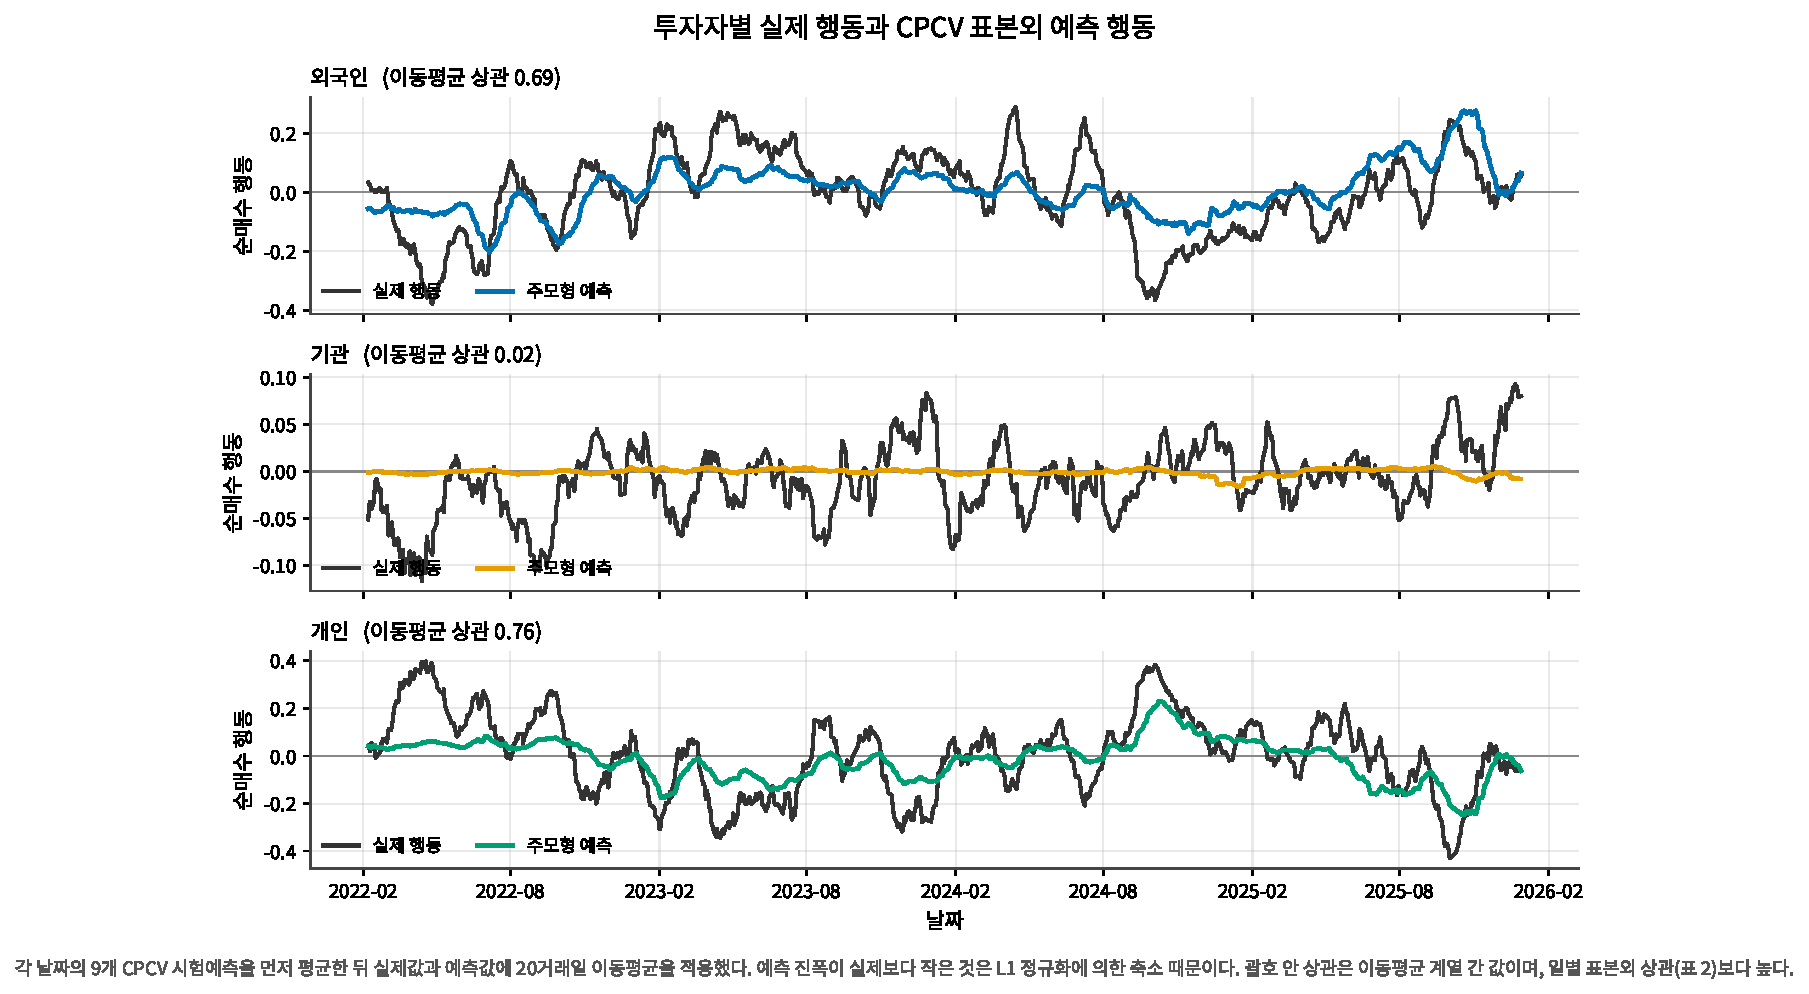
\includegraphics[width=\columnwidth]{../figures_v2/fig2_actual_vs_prediction.pdf}
  \caption{Actual and out-of-sample predicted net buying by investor type. The
  nine CPCV test predictions available for each date are averaged first, then a
  20-day moving average is applied to both the actual and the predicted series.
  Correlations in the panel titles are between the smoothed series and are not
  directly comparable to the daily out-of-sample correlations in
  Table~\ref{tab:performance}.}
  \Description{Three line charts overlaying actual net buying and model
  predictions over time for foreign, institutional and retail investors. In the
  institutional panel the prediction line is flat near zero.}
  \label{fig:prediction}
\end{figure}

Figure~\ref{fig:prediction} places actual and predicted net buying side by side
for the three types. Three things are immediately visible. First, for foreign
and retail investors the predicted series tracks the regime turns of the actual
series, with smoothed correlations of 0.69 and 0.76. Second, the predicted
amplitude is markedly smaller than the actual one, a consequence of coefficient
shrinkage under the $L_1$ penalty. Third, the institutional prediction is
essentially pinned to zero (0.02): the null reported in \S\ref{sec:null} appears
first in the prediction series rather than in a coefficient table.

\begin{table}[t]
  \caption{Out-of-sample performance under CPCV (mean $\pm$ s.d.\ over 45
  splits) and the persistence baseline}
  \label{tab:performance}
  \small
  \centering
  \begin{tabular}{@{}lccc@{}}
    \toprule
    Metric & Foreign & Institutional & Retail \\
    \midrule
    \multicolumn{4}{@{}l}{\emph{Main model}}\\
    Directional accuracy & $0.636\pm0.039$ & $0.542\pm0.038$ & $0.608\pm0.044$ \\
    Correlation          & $0.278\pm0.110$ & $0.068\pm0.064$ & $0.245\pm0.118$ \\
    MAE                  & $0.195\pm0.019$ & $0.094\pm0.008$ & $0.264\pm0.029$ \\
    RMSE                 & $0.246\pm0.021$ & $0.125\pm0.012$ & $0.318\pm0.030$ \\
    MAE / action s.d.    & $0.759$ & $0.756$ & $0.791$ \\
    Saturation rate      & $0.000$ & $0.000$ & $0.000$ \\
    \addlinespace
    \multicolumn{4}{@{}l}{\emph{Persistence baseline} ($a_{t+1}\leftarrow a_t$)}\\
    Directional accuracy & $\mathbf{0.642}$ & $\mathbf{0.547}$ & $\mathbf{0.616}$ \\
    Correlation          & $\mathbf{0.359}$ & $\mathbf{0.136}$ & $\mathbf{0.311}$ \\
    MAE                  & $0.223$ & $0.123$ & $0.299$ \\
    \addlinespace
    Action AR(1)         & $0.401$ & $0.149$ & $0.345$ \\
    \bottomrule
  \end{tabular}
\end{table}

\begin{figure}[t]
  \centering
  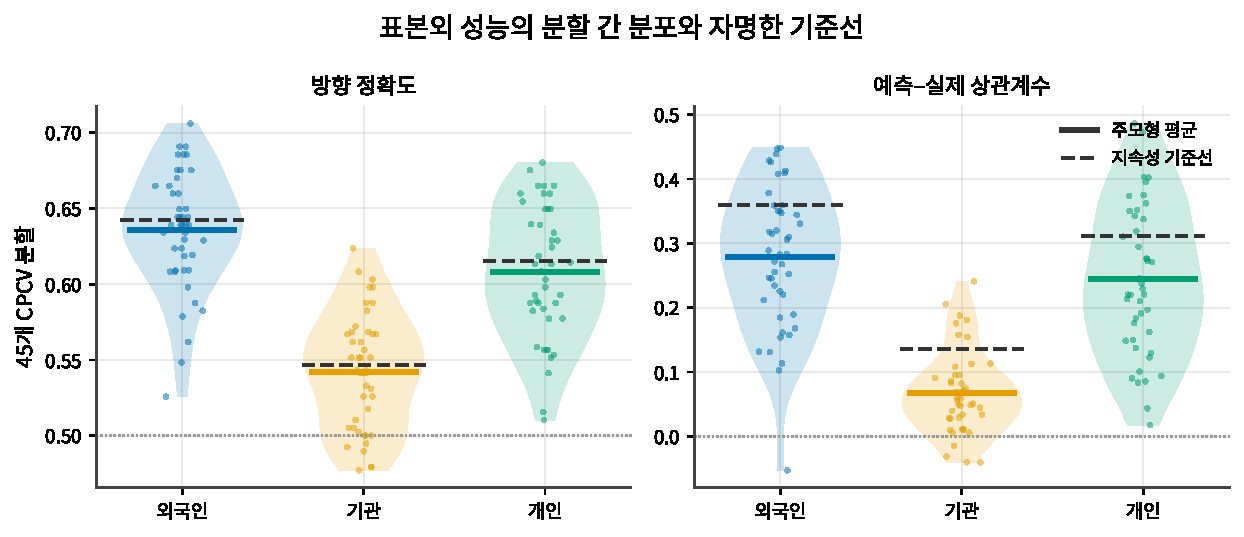
\includegraphics[width=\columnwidth]{../figures_v2/fig5_oos_performance.pdf}
  \caption{Split-level distribution of out-of-sample performance against a naive
  baseline. Solid lines are the main-model mean and dashed lines the persistence
  baseline. The dashed line lies above the solid line for all three types.}
  \Description{Two panels showing violin and point distributions of directional
  accuracy and correlation across 45 splits for the three investor types.}
  \label{fig:oos}
\end{figure}

Table~\ref{tab:performance} and Figure~\ref{fig:oos} reveal two things that
means alone conceal. First, dispersion across splits is large: the foreign
correlation ranges from $-0.05$ to $0.45$, so comparing types from a single
split is meaningless. Second, the naive persistence baseline outperforms the
main model on both directional accuracy and correlation. Since $a_t$ is
published after the day-$t$ close, this is an informationally feasible rule. The
main model leads only on MAE, and because that follows from shrinkage of the
predicted amplitude it cannot be read as an informational advantage.

The reason for the gap is clear. The action has first-order autocorrelation of
$0.401/0.149/0.345$, yet our reward feature set does not include the lagged own
action. Restricting the features to (F1)--(F3) was a design choice ensuring that
all three types share only features corresponding to independently established
behavioural regularities; it was not a design aimed at maximizing predictive
performance. We report this result openly in Table~\ref{tab:performance}.
Table~\ref{tab:performance} and Figure~\ref{fig:oos} are used to show that the
model has not merely fitted noise, not as evidence of predictive superiority.

Because the saturation rate is exactly zero for every type in every split, the
premise $|q|\le1$ of Proposition~\ref{prop:lasso} holds throughout the sample.
The estimator is therefore literally the Lasso of Equation~\eqref{eq:lasso}, and
performance does not rely on extreme $\pm1$ predictions.

\subsection{Recovered Rewards: A Mirror Image on the Momentum Axis}
\label{sec:beta}

\begin{figure*}[t]
  \centering
  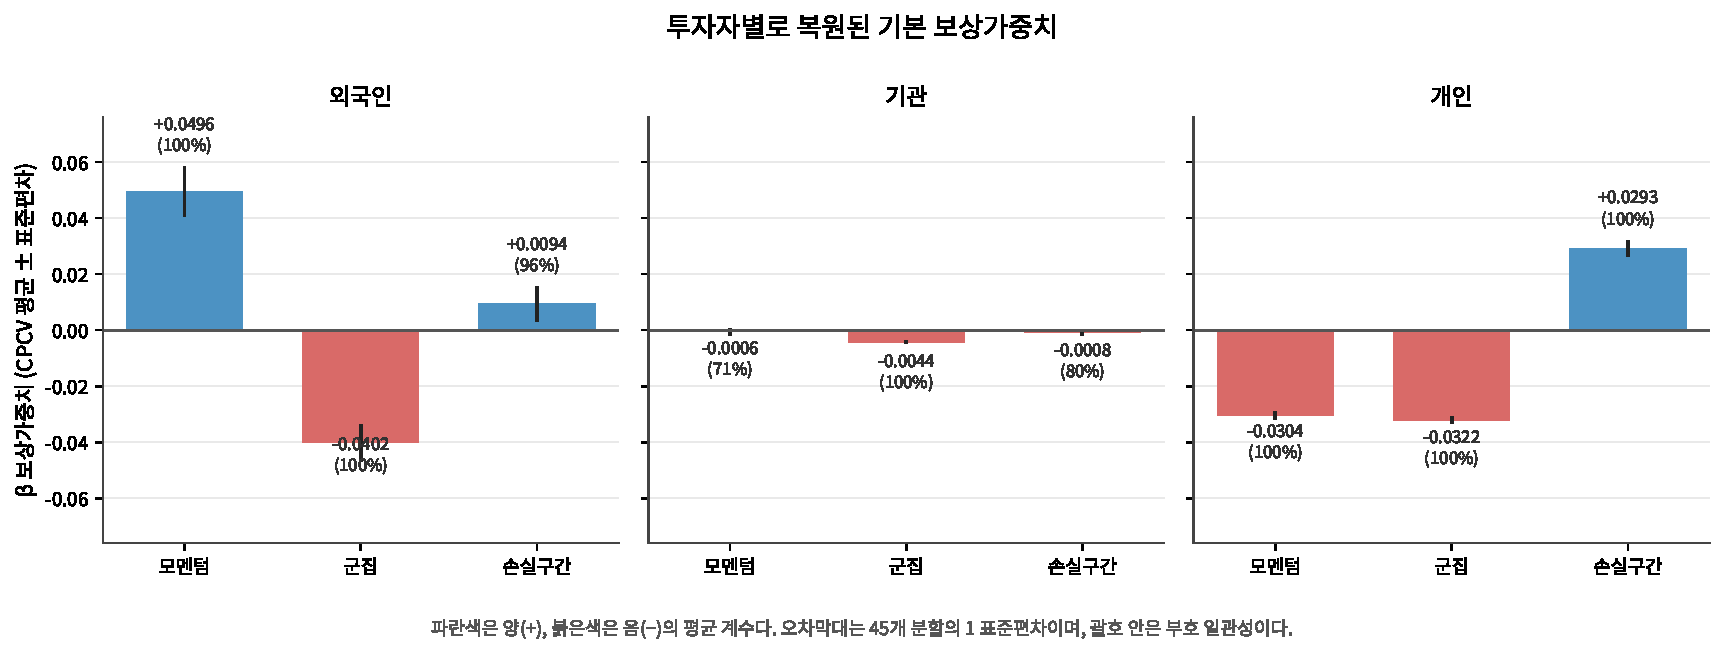
\includegraphics[width=\textwidth]{../figures_v2/fig1_reward_weights_bar.pdf}
  \caption{Recovered baseline reward weights $\beta$ by investor type. Blue bars
  are positive and red bars negative mean coefficients; error bars are one
  standard deviation across the 45 splits and the parenthesised figure is sign
  consistency.}
  \Description{Three bar charts giving momentum, herding and underwater
  coefficients for foreign, institutional and retail investors. Foreign momentum
  is positive, retail momentum negative, and the institutional bars are barely
  visible.}
  \label{fig:betabar}
\end{figure*}

\begin{figure*}[t]
  \centering
  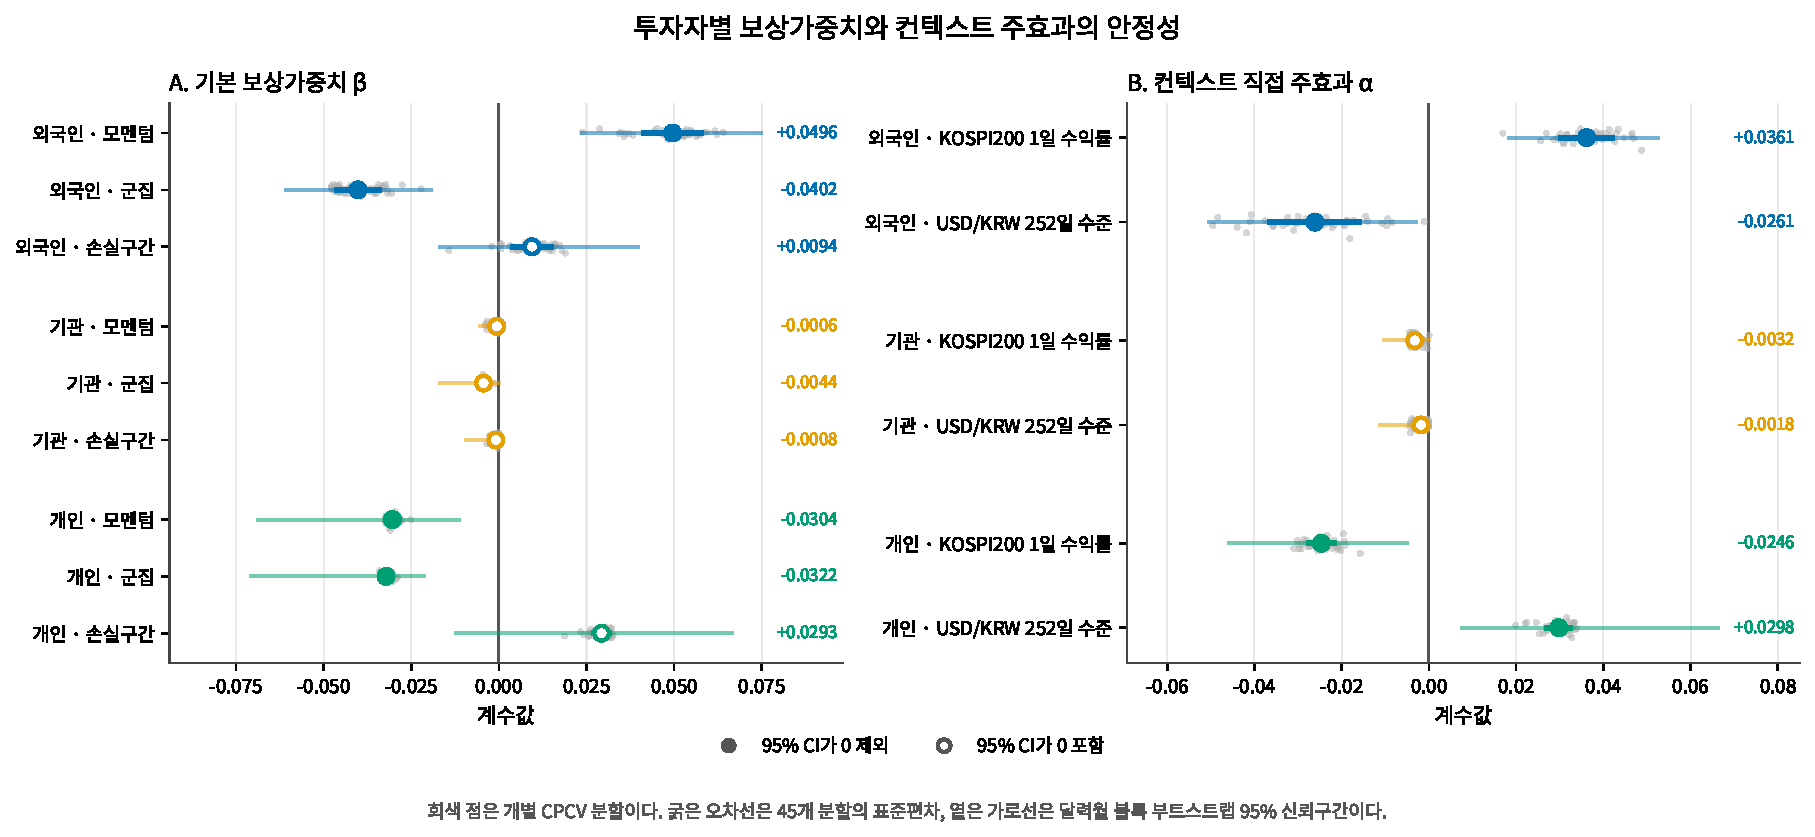
\includegraphics[width=\textwidth]{../figures_v2/fig3_beta_alpha_forest.pdf}
  \caption{Split-level stability of reward weights and context main effects.
  Grey dots are individual CPCV splits, thick error bars the standard deviation
  across the 45 splits, and light horizontal lines the 95\% calendar-month block
  bootstrap interval. Hollow markers denote terms whose interval contains zero.}
  \Description{Forest plots for baseline reward weights (panel A) and context
  main effects (panel B), showing per-split estimates and confidence intervals
  for each term.}
  \label{fig:forest}
\end{figure*}

Figure~\ref{fig:betabar} places the recovered baseline reward weights of the
three types side by side. Because all types received the same feature set and
the same model form and only their parameters were estimated separately, the
differences in bar height are entirely learned from the data.
Figure~\ref{fig:forest} unfolds the same $\beta$ together with the context main
effects $\alpha$ down to the split level.

\paragraph{The mirror image on the momentum axis}
The foreign momentum weight is $+0.0496$ and positive in all 45 splits, while
the retail weight is $-0.0304$ and negative in all 45 splits. In
Figure~\ref{fig:betabar} the two bars point in opposite directions across the
zero line, and in Figure~\ref{fig:forest} their bootstrap intervals do not
overlap and each excludes zero. Although the same feature set was estimated
independently for each type, the two types diverge in exactly opposite
directions on momentum: foreign investors appear as trend followers and retail
investors as contrarians, matching the sign expectations of prior
work~\cite{grinblatt2000investment,choe1999foreign}.

\paragraph{Herding}
The herding coefficient is negative in all 45 splits for all three types, and
the bootstrap intervals of the foreign ($-0.0402$) and retail ($-0.0322$)
coefficients also exclude zero. This result, however, does not separate a
behavioural interpretation from the market-clearing constraint. As
Figure~\ref{fig:crossinv} shows, the same-day correlation between types reaches
$-0.77$, so a substantial part of the negative herding coefficient may arise
mechanically. Because Equation~\eqref{eq:herd} uses a one-day lag the same-day
constraint does not apply directly, but it can propagate through the
autocorrelation of the action. We therefore restrict this result to the
descriptive statement that observed aggregate flow displays a negative
cross-type association, and do not extend it to the behavioural claim that each
type independently trades against the others.

\paragraph{Underwater}
The retail underwater weight is $+0.0293$ and positive in all 45 splits: buying
intensity rises on the following day when the traded price is below the
average-cost proxy, consistent with the reference-price dependence of the
disposition-effect literature~\cite{shefrin1985disposition,odean1998investors}.
The foreign coefficient shares the sign at $+0.0094$ (95.6\%) but is about a
third of the retail magnitude.

As Figure~\ref{fig:forest} shows, however, the underwater bootstrap interval
contains zero for all three types. The retail interval is
$[-0.0122,+0.0665]$: although the sign is 100\% consistent across the 45 splits,
it flips in 5.5\% of month-block resamples. This is exactly the situation
anticipated in \S\ref{sec:protocol}, where sign consistency understates
uncertainty because CPCV splits share observations. We therefore report that a
sign consistent with the disposition effect was observed, but do not claim it as
a statistically established result.

\subsection{Context Response: The Mirror Image Reappears}
\label{sec:alpha}

The mirror image observed on the momentum axis reappears in the context main
effects (panel B of Figure~\ref{fig:forest}). Foreign investors shift toward net
buying on days when the market rises ($+0.0361$) and toward net selling when the
won is weak ($-0.0261$), while retail investors do exactly the opposite on both
contexts ($-0.0246$ and $+0.0298$). All four coefficients keep their sign in all
45 splits and all four bootstrap intervals exclude zero. The two institutional
coefficients have sign consistency above 95\% but are about an eighth of the
foreign and retail magnitudes, and their intervals contain zero.

This mirror image requires the same interpretive reservation as the herding
coefficient. Given the $-0.772$ correlation in Figure~\ref{fig:crossinv}, two
types responding to context with opposite signs may in part reflect the
market-clearing constraint. We therefore present this as the descriptive fact
that the two types form opposite sides of order flow across market and exchange
rate conditions.

\paragraph{Interactions}
Of the twelve interaction coefficients, four keep their sign in all 45 splits:
foreign momentum $\times$ KOSPI200 ($-0.0139$), retail momentum $\times$ FX
($+0.0144$), retail herding $\times$ KOSPI200 ($-0.0080$) and retail
underwater $\times$ FX ($-0.0186$). Only the first and the last of these pass
the bootstrap. Since twelve coefficients were examined jointly, we present the
interactions as exploratory results only.

\subsection{Results of the Stability Protocol}
\label{sec:stability}

\paragraph{(V2) Calendar-month block bootstrap}
The light horizontal lines in Figure~\ref{fig:forest} give this result. The
bootstrap is a stricter criterion than CPCV sign consistency, and the outcome
splits three ways. First, the momentum mirror and the context mirror survive:
eight terms, comprising foreign and retail momentum, herding, and both context
main effects, all exclude zero. Second, the underwater weights do not survive.
Third, no institutional term excludes zero; all six institutional markers in
Figure~\ref{fig:forest} are hollow.

\begin{figure*}[t]
  \centering
  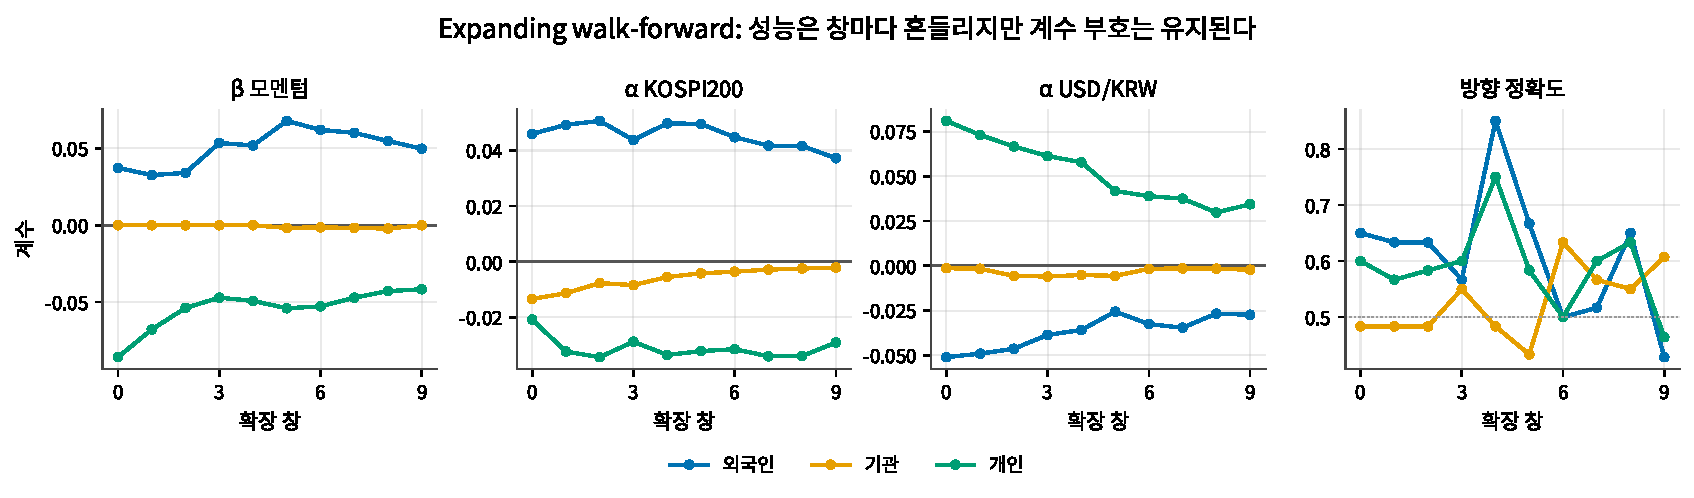
\includegraphics[width=\textwidth]{../figures_v2/fig6_walk_forward.pdf}
  \caption{Coefficient paths and directional accuracy over ten expanding
  walk-forward windows. Performance fluctuates from window to window while the
  coefficient signs hold.}
  \Description{Four line charts against the expanding-window index showing the
  momentum coefficient, the two context main effects, and directional accuracy
  for the three investor types.}
  \label{fig:walkforward}
\end{figure*}

\paragraph{(V3) Expanding walk-forward}
Figure~\ref{fig:walkforward} gives this result, and two things read at once.
Performance fluctuates sharply across windows: foreign directional accuracy
moves between 0.43 and 0.85, averaging $0.610\pm0.116$, and the correlation
falls to $0.131\pm0.162$, less than half the CPCV value of 0.278; retail falls
from 0.245 to 0.129. Because CPCV can place a test fold ahead of a training fold
while walk-forward cannot, we report this degradation as a generalization limit
arising from the temporal structure.

The coefficient paths, by contrast, do not fluctuate. The foreign momentum
coefficient is positive in all ten windows and the retail one negative in all
ten, and the two paths never cross. The same mirror image persists across all
windows for both context main effects, while the three institutional paths stay
pinned near zero. Performance moves with time; the direction of the recovered
preference does not.

\begin{figure*}[t]
  \centering
  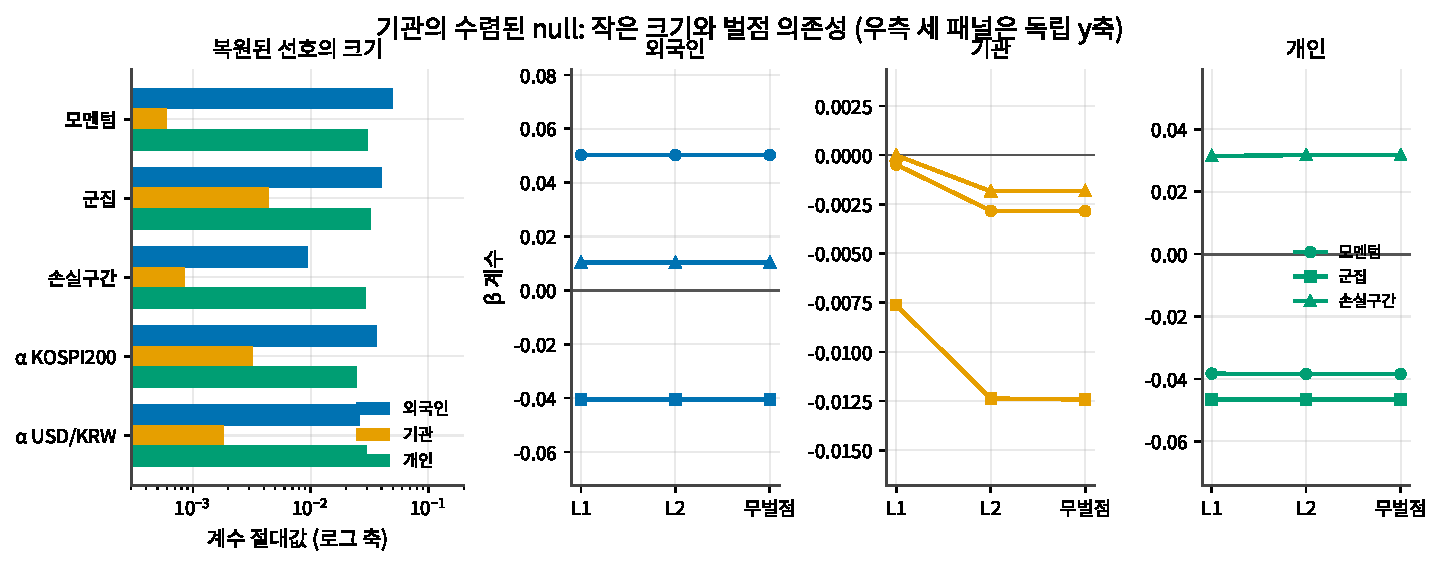
\includegraphics[width=\textwidth]{../figures_v2/fig7_institution_null.pdf}
  \caption{The converged institutional null. Left: magnitude of the recovered
  preferences on a logarithmic axis. Right: sensitivity to the regularization
  swap, with an independent $y$ axis in each of the three panels.}
  \Description{A logarithmic bar chart of coefficient magnitudes by type on the
  left, and three line charts of coefficients under L1, L2 and no penalty on the
  right.}
  \label{fig:null}
\end{figure*}

\paragraph{(V4) Regularization swap}
Figure~\ref{fig:null} gives this result. The foreign and retail coefficients are
effectively invariant to the choice of penalty, agreeing to four decimal places,
so the momentum mirror is not an artefact of the $L_1$ penalty. Only the
institutional coefficients move with the penalty (herding
$-0.0076\rightarrow-0.0124$, underwater $-0.0000\rightarrow-0.0018$), on a
$y$-axis range about one twentieth of that of the other two types. That the
coefficients depend on the choice of penalty means the data do not determine
their value.

\subsection{Institutional Investors: A Converged Null}
\label{sec:null}

For institutional order flow we find no preference that is stably identified at
daily frequency, and we report this as a finding rather than concealing it. The
evidence is fivefold and all of it is visible in the figures.

\begin{enumerate}
\item \textbf{Degenerate prediction.} In the middle panel of
Figure~\ref{fig:prediction} the institutional prediction stays on the zero line
while the actual series moves between $\pm0.1$.
\item \textbf{Magnitude.} In Figure~\ref{fig:betabar} the three institutional
bars are barely visible on the shared axis. Excluding herding, momentum is
$-0.0006$ and underwater $-0.0008$, about one fortieth of the other types.
\item \textbf{Uncertainty.} All six institutional markers in
Figure~\ref{fig:forest} are hollow.
\item \textbf{Penalty dependence.} In the middle right panel of
Figure~\ref{fig:null}, only the institutional coefficients move with the
penalty.
\item \textbf{Temporal instability.} In Figure~\ref{fig:walkforward} the
institutional paths hug the zero line; momentum sign consistency is 40\% of ten
windows and underwater 0\%.
\end{enumerate}

\begin{figure*}[t]
  \centering
  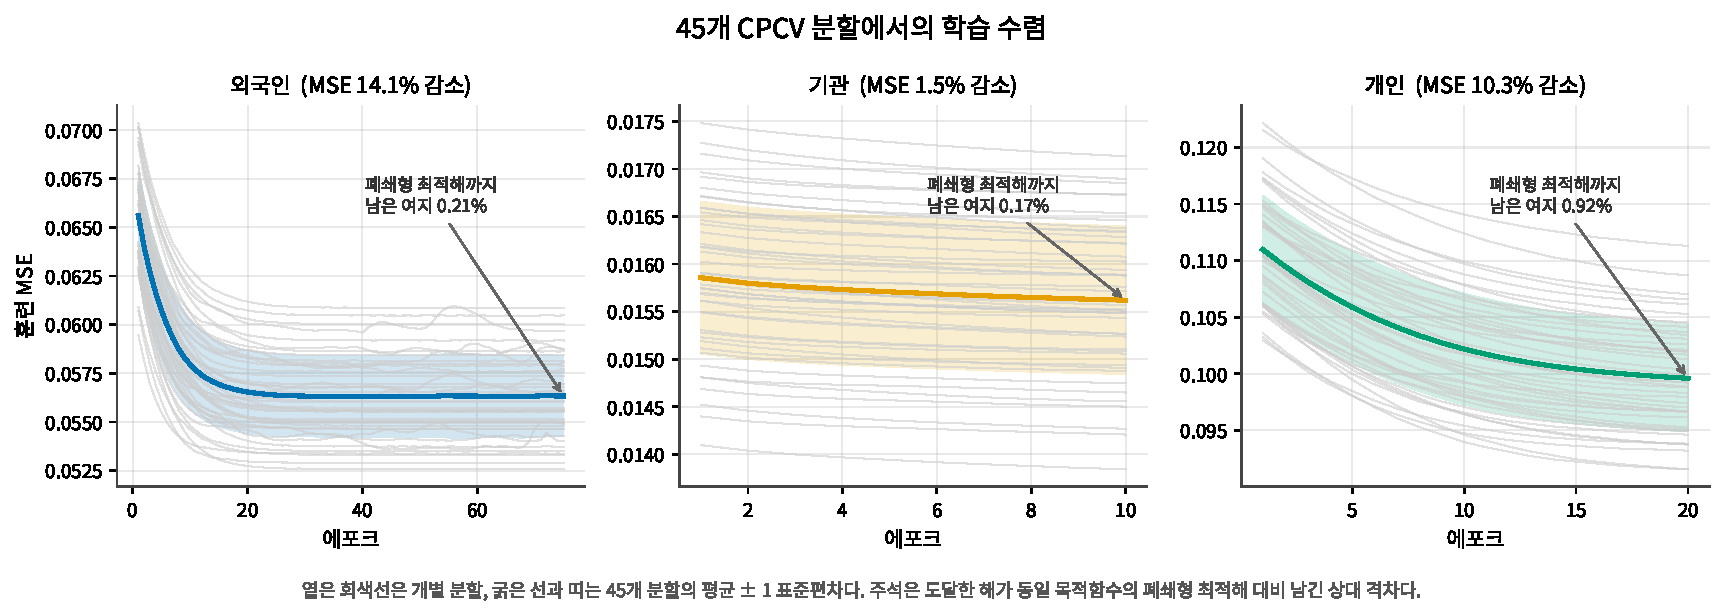
\includegraphics[width=\textwidth]{../figures_v2/fig4_training_convergence.pdf}
  \caption{Training convergence across the 45 CPCV splits. Light grey lines are
  individual splits; the thick line and band are the mean $\pm$ one standard
  deviation. The annotation gives the relative gap between the solution reached
  and the closed-form optimum of the same objective.}
  \Description{Three panels of training MSE against epoch for the three investor
  types; the institutional panel shows the smallest decrease.}
  \label{fig:convergence}
\end{figure*}

This null is not an optimization failure. Figure~\ref{fig:convergence} shows the
training curves across the 45 splits. The institutional training MSE falls by
only 1.5\% over the whole training run and the curve does not look visually
flat. That is not underfitting, however, but the fact that there is almost no
error left to remove. By Proposition~\ref{prop:lasso}, Equation~\eqref{eq:loss}
is convex with a unique global optimum, and comparing the solution reached with
the closed-form optimum of the same objective leaves an institutional gap of
only 0.17\% on average and 0.48\% at most (0.21\% for foreign and 0.92\% for
retail). All three types reach the attainable optimum; only for institutional
investors do the coefficients at that optimum sit near zero. The data do not
determine an institutional preference; it is not that the optimizer failed to
find one.

Economically the null reads naturally. The ``institutional'' category aggregates
pension funds, investment trusts, insurers, private funds, and securities firms,
so the flows of agents with different objective functions offset one another.
The one consistently negative herding coefficient is compatible with a shared
liquidity-provision role on the opposite side of the other types, but because
its bootstrap interval sits on the boundary we do not claim it.

\subsection{Construct Validity Check}
\label{sec:construct}

\begin{table}[t]
  \caption{Prior sign expectations and recovered results}
  \label{tab:construct}
  \small
  \begin{tabular}{@{}>{\raggedright\arraybackslash}p{0.26\columnwidth}
                  >{\raggedright\arraybackslash}p{0.14\columnwidth}
                  >{\raggedright\arraybackslash}p{0.24\columnwidth}
                  >{\raggedright\arraybackslash}p{0.20\columnwidth}@{}}
    \toprule
    Regularity & Expected & Recovered & Verdict \\
    \midrule
    Foreign trend trading~\cite{grinblatt2000investment,choe1999foreign}
      & $\beta^{mom}>0$ & $+0.0496$ (100\%, CI excl.\ 0) & matches \\
    Retail contrarian trading~\cite{grinblatt2000investment,kaniel2008individual}
      & $\beta^{mom}<0$ & $-0.0304$ (100\%, CI excl.\ 0) & matches \\
    Disposition effect~\cite{shefrin1985disposition,odean1998investors}
      & $\beta^{uw}>0$ & $+0.0293$ (100\%, CI incl.\ 0) & partial \\
    Institutional herding~\cite{lakonishok1992impact}
      & $\beta^{herd}>0$ & $-0.0044$ (100\%, CI incl.\ 0) & mismatch \\
    \bottomrule
  \end{tabular}
\end{table}

Table~\ref{tab:construct} reports the contrast. Although all three types
received the same features and the same model form and only their parameters
were estimated separately, the recovered signs agree with independently
established regularities and the two types diverge in opposite directions on
momentum. This is evidence of construct validity: the recovered reward is not an
arbitrary fit.

The mismatch arises because the measured object differs. Lakonishok et
al.~\cite{lakonishok1992impact} measure the extent to which agents \emph{within}
the institutional group move in the same direction, whereas
Equation~\eqref{eq:herd} measures whether institutions move with the previous
day's flow of the \emph{other two types}. Our result is therefore not a
refutation of that literature; testing within-type herding would require data on
institutional sub-categories.

\subsection{What This Study Does Not Claim}
\label{sec:notclaim}

As the final stage of the protocol we state explicitly what the results do not
support.

\begin{enumerate}
\item \textbf{Return predictability.} Our metrics are reproduction errors for
the direction and intensity of order flow and include no returns, Sharpe ratios,
or transaction costs. No trading rule follows from
Table~\ref{tab:performance}.

\item \textbf{Superior flow prediction.} As reported in
Table~\ref{tab:performance} and Figure~\ref{fig:oos}, the persistence baseline
beats the main model on directional accuracy and correlation. Our objective is
preference recovery on an interpretable common scale rather than predictive
performance, and the two objectives call for different feature sets. In a
preliminary check, adding the lagged own action as a fourth feature lifts the
model above the baseline (directional accuracy $0.646/0.569/0.629$) but reverses
the sign of the retail $\alpha^{KOSPI}$ and eliminates the underwater
coefficient. Some of the mirror images reported here are therefore not separable
from the autocorrelation of order flow.

\item \textbf{Causal effects.} The recovered weights are conditional
associations among standardized observed features. Because feature--context
correlations range from $-0.29$ to $0.22$ (Figure~\ref{fig:featcorr}), the
magnitude of any coefficient depends on the other terms being controlled for.

\item \textbf{A behavioural reading of the negative cross-type association.} The
herding coefficient and the mirrored context responses are not separable from
the market-clearing constraint (Figure~\ref{fig:crossinv}).

\item \textbf{A test of the disposition effect.} The retail underwater sign
agrees with the literature but does not pass the month-block bootstrap
(Figure~\ref{fig:forest}), and the average-cost proxy is built from aggregate
trades rather than account-level realized gains and holding periods.

\item \textbf{Generalization across stocks.} The single-stock design is a
control for isolating heterogeneity across types; extension to other stocks and
markets is untested.
\end{enumerate}

% =====================================================================
\appendix

\section{Supplementary Material}
\label{sec:appendix}

This appendix collects the supporting figures and tables referenced in the main
text. Figure~\ref{fig:saturation} verifies the premise of
Proposition~\ref{prop:lasso}, Figure~\ref{fig:featcorr} reports
feature--context correlations, and Figure~\ref{fig:crossinv} shows same-day
actions across types. Table~\ref{tab:interactions} lists the full set of
interaction coefficients presented as exploratory in the main text, and
Table~\ref{tab:convergence} reports the optimality check of the solution
reached.

\begin{figure}[htbp]
  \centering
  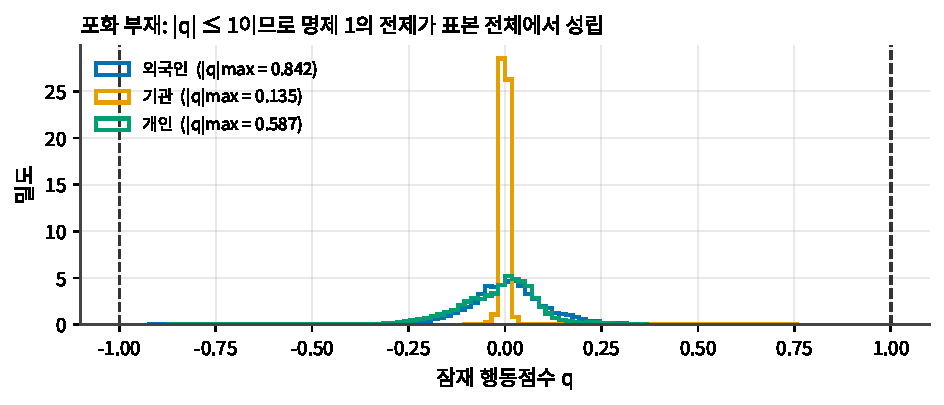
\includegraphics[width=\columnwidth]{../figures_v2/figA1_no_saturation.pdf}
  \caption{Distribution of the latent action score against the action bounds.
  Since $|q|\le1$, the premise of Proposition~\ref{prop:lasso} holds throughout
  the sample and the saturation rate is exactly zero in all 45 splits.}
  \Description{Histograms of the latent action score for the three types with
  the $\pm1$ bounds marked.}
  \label{fig:saturation}
\end{figure}

\begin{figure}[htbp]
  \centering
  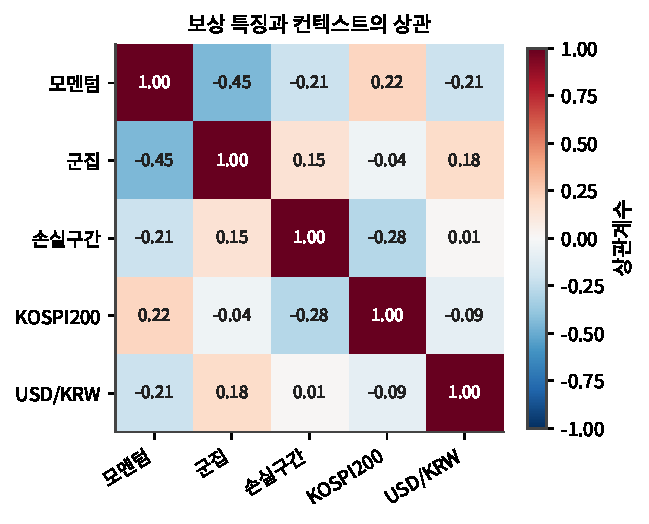
\includegraphics[width=\columnwidth]{../figures_v2/figA2_feature_correlation.pdf}
  \caption{Correlation matrix of reward features and contexts (foreign features,
  973 observations).}
  \Description{A heatmap showing correlation coefficients among five variables
  in colour and numerals.}
  \label{fig:featcorr}
\end{figure}

\begin{figure}[htbp]
  \centering
  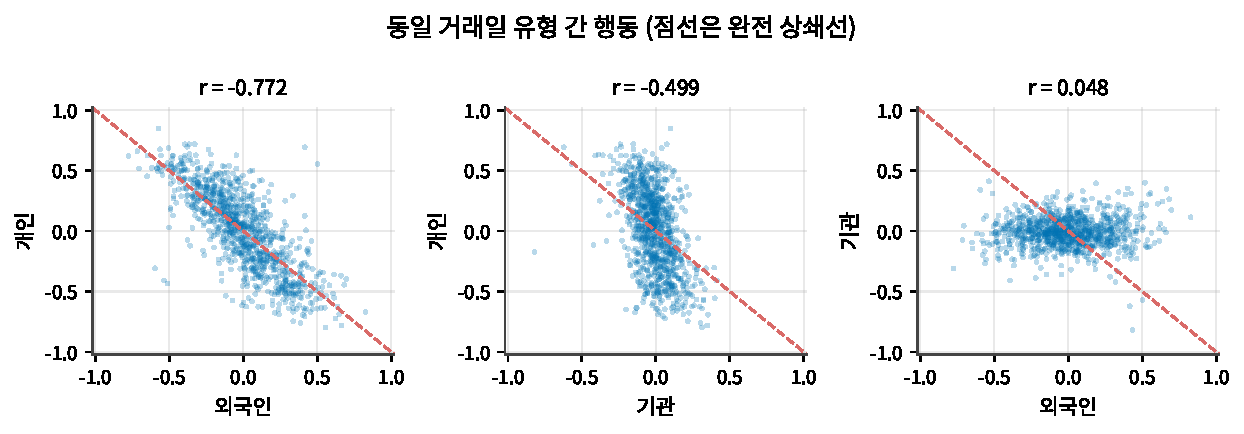
\includegraphics[width=\columnwidth]{../figures_v2/figA3_cross_investor_actions.pdf}
  \caption{Same-day actions across investor types. The dashed line marks perfect
  offset; foreign and retail actions cluster along it.}
  \Description{Three scatter plots of actions for each pair of investor types
  with the corresponding correlation coefficients.}
  \label{fig:crossinv}
\end{figure}

\begin{table}[htbp]
  \caption{Interaction coefficients $B$ (45 splits)}
  \label{tab:interactions}
  \small
  \centering
  \begin{tabular}{@{}llrrr@{}}
    \toprule
    Type & Feature $\times$ context & Mean & S.d. & Sign cons. \\
    \midrule
    Foreign & momentum $\times$ KOSPI200 & $-0.0139$ & $0.0052$ & 100.0\% \\
    Foreign & momentum $\times$ FX       & $-0.0030$ & $0.0057$ & 71.1\% \\
    Foreign & herding $\times$ KOSPI200  & $+0.0016$ & $0.0074$ & 66.7\% \\
    Foreign & herding $\times$ FX        & $+0.0037$ & $0.0073$ & 68.9\% \\
    Foreign & underwater $\times$ KOSPI200 & $-0.0062$ & $0.0040$ & 93.3\% \\
    Foreign & underwater $\times$ FX     & $-0.0075$ & $0.0076$ & 86.7\% \\
    \addlinespace
    Inst. & momentum $\times$ KOSPI200 & $-0.0001$ & $0.0005$ & 66.7\% \\
    Inst. & momentum $\times$ FX       & $+0.0003$ & $0.0006$ & 80.0\% \\
    Inst. & herding $\times$ KOSPI200  & $-0.0004$ & $0.0006$ & 86.7\% \\
    Inst. & herding $\times$ FX        & $+0.0012$ & $0.0012$ & 93.3\% \\
    Inst. & underwater $\times$ KOSPI200 & $+0.0028$ & $0.0012$ & 97.8\% \\
    Inst. & underwater $\times$ FX     & $+0.0007$ & $0.0008$ & 91.1\% \\
    \addlinespace
    Retail & momentum $\times$ KOSPI200 & $+0.0021$ & $0.0042$ & 80.0\% \\
    Retail & momentum $\times$ FX       & $+0.0144$ & $0.0045$ & 100.0\% \\
    Retail & herding $\times$ KOSPI200  & $-0.0080$ & $0.0046$ & 100.0\% \\
    Retail & herding $\times$ FX        & $+0.0092$ & $0.0081$ & 82.2\% \\
    Retail & underwater $\times$ KOSPI200 & $-0.0022$ & $0.0046$ & 66.7\% \\
    Retail & underwater $\times$ FX     & $-0.0186$ & $0.0046$ & 100.0\% \\
    \bottomrule
  \end{tabular}
\end{table}

\begin{table}[htbp]
  \caption{Optimality check of the solution reached (45 splits)}
  \label{tab:convergence}
  \small
  \centering
  \begin{tabular}{@{}lccc@{}}
    \toprule
    Type & MSE drop & Gap (\%) & Cosine \\
     & (training) & mean / max & mean / min \\
    \midrule
    Foreign & 14.1\% & $0.21/3.10$ & $0.994/0.948$ \\
    Inst.   & 1.5\%  & $0.17/0.48$ & $0.935/0.832$ \\
    Retail  & 10.3\% & $0.92/1.40$ & $0.894/0.833$ \\
    \bottomrule
  \end{tabular}
\end{table}

%  Required packages: booktabs, graphicx, amsmath, array, url
%  Figure path: ../figures_v2/  (output of scripts/make_paper_figures.py)
%  Additional references: merge paper-refs-additional.bib
% =====================================================================

\section{Method}
\label{sec:method}

\subsection{Setup: Symmetric Estimation}
\label{sec:setup}

Let the set of investor types be
$\mathcal{I}=\{\text{foreign},\text{institutional},\text{retail}\}$. Each type is
treated as an agent whose observed daily order flow reveals a latent reward
defined over interpretable market state features.

\paragraph{Continuous action}
Writing $V^{buy}_{i,t}$ and $V^{sell}_{i,t}$ for the daily gross buy and gross
sell value of type $i$, we define the action as
\begin{equation}
u_{i,t}=\frac{V^{buy}_{i,t}-V^{sell}_{i,t}}
             {V^{buy}_{i,t}+V^{sell}_{i,t}}\in[-1,1].
\label{eq:action}
\end{equation}
Because the denominator is the type's own gross turnover rather than
market-wide turnover, $u_{i,t}$ measures whether buying or selling dominated
\emph{within} that type, giving a common scale that is unaffected by
differences in trading size across types. Using a continuous intensity rather
than a binary buy/sell label preserves the magnitude information that
dichotomization discards.

\paragraph{Symmetry}
All three types receive the same state features $x_{i,t}\in\mathbb{R}^{3}$, the
same market context $C_t\in\mathbb{R}^{2}$, and the same model form. No type is
assigned a different feature a priori; only the parameters
$\theta_i=(\beta_i,B_i,\alpha_i)$ are estimated separately on each type's own
data. Any difference that appears in the results is therefore learned from the
data rather than imposed by design, and this symmetry is what licenses direct
comparison of coefficients across types.

\paragraph{Timing}
The training sample is $(x_{i,t},C_t,a_{i,t+1})$ with $a_{i,t+1}=u_{i,t+1}$. A
state built from day-$t$ closing prices and order flow explains day-$t+1$
behaviour, so no future trade enters the features. Momentum and underwater use
day-$t$ information while the herding feature uses day $t-1$. Since the target
is day-$t+1$ behaviour, day-$t$ information is also available; the extra lag on
herding is therefore not an information constraint but a design choice that
keeps the same-day accounting offset between types out of the predictor set
(Figure~\ref{fig:crossinv}).

\subsection{Reward Features}
\label{sec:features}

All three features are standardized using statistics fitted on the training
indices of each validation split only. Every coefficient reported below is
therefore read as the effect of a one-standard-deviation move of that feature
within the training window.

\paragraph{(F1) Medium-term momentum}
With adjusted (or fallback) closing price $P_t$,
\begin{equation}
x^{mom}_{i,t}=\log\!\left(\frac{P_t}{P_{t-20}}\right).
\label{eq:momentum}
\end{equation}
Twenty trading days is a pre-specified window of roughly one month, chosen to
damp daily price noise while still expressing a medium-term trend linked to
next-day behaviour. It is a design value for interpretability, not a value tuned
on the data. A positive coefficient indicates trend following and a negative one
contrarian trading; the sign expectation follows prior work on type-specific
momentum trading~\cite{grinblatt2000investment,choe1999foreign}.

\paragraph{(F2) Herding}
The cross-sectional average of the previous day's actions of the two types other
than $i$:
\begin{equation}
x^{herd}_{i,t}=\frac{u_{j,t-1}+u_{k,t-1}}{2},\qquad j,k\neq i.
\label{eq:herd}
\end{equation}
Note that this is an average across the two other types at one point in time,
not a time average. A 20-day moving average would measure a month of cumulative
flow pressure rather than an immediate response, so we focus on the previous
day. A positive coefficient means moving with the previous day's direction of
the other types, a negative one means moving against it. The sign expectation
follows the institutional herding
literature~\cite{lakonishok1992impact}; note however that this literature
measures herding \emph{within} the institutional group, whereas
Equation~\eqref{eq:herd} measures a relation \emph{between} types
(\S\ref{sec:construct}).

\paragraph{(F3) Underwater gap relative to average cost}
With a per-type average-cost proxy $\bar P_{i,t}$ and the day's gross-trade VWAP
$P^{vwap}_{i,t}$,
\begin{equation}
x^{uw}_{i,t}=\max\!\left(
\frac{\bar P_{i,t}-P^{vwap}_{i,t}}{\bar P_{i,t}},\,0\right).
\label{eq:underwater}
\end{equation}
Truncation at zero makes the feature active only when the traded price sits
below the average-cost proxy, so the variable is reference-point dependent by
construction. The average cost is obtained by recursively updating an effective
inventory from gross buy and sell quantities and values: the previous day's
inventory is multiplied by a forgetting factor $\rho=0.98$ to damp the influence
of old trades, and sales do not change the average cost of the remaining
position. With $\rho=0.98$ the half-life is about 34 trading days and roughly
66.8\% remains after 20, so the feature emphasises the trading memory of the
past one to two months; this value was also not tuned on the data. A positive
coefficient means stronger next-day buying below the average cost, and the sign
expectation follows the disposition-effect
literature~\cite{shefrin1985disposition,odean1998investors}.

The proxy is constructed from aggregate flow rather than actual account
holdings. Buys and sells executed by different accounts within the same type
net out, so the notion of a ``representative investor's average cost'' is itself
an approximation. The coefficient on $x^{uw}$ therefore cannot be read as a
direct test of the disposition effect.

\subsection{Market Context}
\label{sec:context}

The context consists of two variables: (C1) the one-day KOSPI200 return $r_t$,
and (C2) the KRW/USD exchange rate level
\begin{equation}
z_t=\frac{\log e_t-\mu_{t-1,252}}{\sigma_{t-1,252}},
\label{eq:fxcontext}
\end{equation}
where the current rate is used but the mean and standard deviation are computed
only through $t-1$ over 252 trading days. Both contexts are likewise
re-standardized on the training indices of each split, so their coefficients
read as the effect of a one-standard-deviation move within the training window.

Context and reward features are not independent. Because Samsung Electronics
carries a large weight in the KOSPI200, stock momentum overlaps with the market
return, and feature--context correlations range from $-0.29$ to $0.22$
(Figure~\ref{fig:featcorr}). Individual coefficients are therefore conditional
associations given the other terms and should not be read as causal magnitudes
in isolation.

\subsection{Myopic Reward, Policy, and the Reduction to Lasso}
\label{sec:model}

\paragraph{Latent action score}
Define the action score of type $i$ at time $t$ as
\begin{equation}
q_{i,t}=(\beta_i+B_iC_t)^{\top}x_{i,t}+\alpha_i^{\top}C_t,
\label{eq:score}
\end{equation}
where $\beta_i\in\mathbb{R}^{3}$ is the baseline reward weight at average
context, $B_i\in\mathbb{R}^{3\times 2}$ the feature--context interaction, and
$\alpha_i\in\mathbb{R}^{2}$ the direct context main effect. The $\alpha$ term is
a level effect that shifts behaviour even when the stock features are at their
means; the $B$ term is a slope effect that changes sensitivity to each feature
across market conditions. Including interaction terms while omitting the
lower-order term $C_t$ is a standard specification error, so the inclusion of
$\alpha$ is required by the specification rather than something to be justified
empirically.

\paragraph{Myopic concave reward}
The one-step reward for a continuous action $a$ is
\begin{equation}
R_i(x,C,a)=q_{i,t}\,a-\frac{\kappa}{2}a^{2}.
\label{eq:reward}
\end{equation}
The quadratic term imposes a symmetric cost on large net buying and net selling
and makes the reward concave in the action, which permits an interior solution.
Without it, maximizing over $[-1,1]$ would return $\pm1$ almost always depending
only on the sign of $q$, and the \emph{intensity} of behaviour could not be
reproduced. Maximizing Equation~\eqref{eq:reward} over $a$ yields the closed-form
policy
\begin{equation}
a^{*}_{i,t+1}=\mathrm{clip}\!\left(\frac{q_{i,t}}{\kappa},-1,1\right).
\label{eq:policy}
\end{equation}
The curvature $\kappa$ is fixed at one for identification. With $\kappa=2$ the
same $q$ would halve the action size, but re-estimation would double the
coefficients of $q$ and reproduce the same behaviour; $\kappa=1$ therefore fixes
the units of the reward and the coefficients rather than asserting that the
empirical curvature equals one.

\paragraph{Estimation}
The training objective for each type on its training set $\mathcal{D}_i$ is
\begin{equation}
\min_{\theta_i}\ \frac{1}{|\mathcal{D}_i|}
\sum_{t\in\mathcal{D}_i}\bigl(a^{*}_{i,t+1}-a_{i,t+1}\bigr)^{2}
+\lambda_i\lVert\theta_i\rVert_1,
\label{eq:loss}
\end{equation}
optimized independently per type with Adam~\cite{kingma2015adam}.

\begin{proposition}[Reduction to Lasso]
\label{prop:lasso}
Let
$z_{i,t}=[\,x_{i,t};\ \mathrm{vec}(x_{i,t}C_t^{\top});\ C_t\,]\in\mathbb{R}^{11}$
and $\theta_i=[\,\beta_i;\ \mathrm{vec}(B_i);\ \alpha_i\,]$, so that
Equation~\eqref{eq:score} reads $q_{i,t}=\theta_i^{\top}z_{i,t}$. If
$|q_{i,t}|\le 1$ throughout the training sample, the clip in
Equation~\eqref{eq:policy} never binds, $a^{*}=q$, and
Equation~\eqref{eq:loss} becomes
\begin{equation}
\min_{\theta_i}\ \frac{1}{|\mathcal{D}_i|}
\sum_{t}\bigl(\theta_i^{\top}z_{i,t}-a_{i,t+1}\bigr)^{2}
+\lambda_i\lVert\theta_i\rVert_1,
\label{eq:lasso}
\end{equation}
which is exactly an $L_1$-penalized (Lasso) regression of next-day net-buying
intensity on the expanded state feature $z$.
\end{proposition}

Under a myopic concave reward with $\kappa=1$, ``recovering a preference'' and
``regressing order flow'' are therefore numerically indistinguishable.
Figure~\ref{fig:saturation} shows that the premise of
Proposition~\ref{prop:lasso} in fact holds in our sample: for all three types the
distribution of the latent action score sits far inside the action bounds
$\pm1$ (the maximum $|q|$ is 0.842 for foreign, 0.587 for retail and 0.135 for
institutional investors), and the saturation rate is exactly zero in all 45
splits.

\paragraph{Why we do not hide the reduction}
This coincidence is not a weakness of the method but a logical consequence of
the myopia assumption. If the agent looks only one step ahead, today's action
does not affect anything beyond tomorrow, so there is no future to look toward
and \emph{what the agent wants} (the reward) collapses onto \emph{what the agent
does} (the policy). Applying the stochastic policy of maximum-entropy
IRL~\cite{ziebart2008maximum}, $\pi(a\mid x,C)\propto\exp(R/\tau)$, to
Equation~\eqref{eq:reward} makes $\pi$ a truncated normal with mean $q$ and
variance $\tau$, whose maximum-likelihood point estimate coincides with
Equation~\eqref{eq:lasso}. The reduction is thus a property of the myopic,
quadratic-reward setting in general, not an artefact of one implementation.

The distinctive value of the inverse reinforcement learning formulation lies in
the extension path. Once state dynamics and multi-period value are introduced,
the reward separates from the policy and leads to a structural recovery that
regression cannot reach. This paper is the first step on that path, and it adds
interpretation and validation on top of an explicitly stated set of conditions.

\subsection{Validation Protocol}
\label{sec:protocol}

Rather than stopping at the sign and magnitude of the recovered coefficients, we
apply four stages.

\begin{description}
\item[(V1) Out-of-sample stability under CPCV] We use combinatorial purged
cross-validation~\cite{lopez2018advances} with ten temporal folds of which two
serve as test folds, giving $\binom{10}{2}=45$ splits, a one-day purge and a
five-day embargo between training and test, and all standardization fitted on
training indices only. We report the fraction of splits in which the dominant
sign appears (sign consistency), but because the splits share observations we
interpret sign consistency only as a stability indicator, never as an
independent-sample $p$-value.

\item[(V2) Calendar-month block bootstrap] To address the fact that sign
consistency is not a test, we partition the sample into calendar-month blocks,
resample months with replacement, and re-estimate 1{,}000 times to obtain 95\%
confidence intervals. Month blocks preserve the autocorrelation of daily flow
and within-month patterns inside each block.

\item[(V3) Expanding walk-forward] Because CPCV can place a test fold before a
training fold, we add a validation that strictly respects the arrow of time. We
train on the first 400 observations, predict the next 60 trading days after a
five-day purge, and repeat while expanding the training window by 60 trading
days, for ten windows in total.

\item[(V4) Regularization swap] To confirm that the results are not an artefact
of the $L_1$ penalty, we re-run the same protocol with an $L_2$ penalty and with
no penalty, and compare coefficient signs.
\end{description}

\paragraph{Metrics}
Magnitude error is measured by MAE and RMSE, and directional reproduction by
directional accuracy, the fraction of days with
$\mathrm{sign}(a^{*})=\mathrm{sign}(a)$. We also report the Pearson correlation
between actual and predicted actions and the saturation rate, the fraction with
$|a^{*}|=1$. Because action standard deviations differ across types, absolute
MAE and RMSE are not compared across types but interpreted within each type, and
we report errors normalized by the action standard deviation alongside them. As
a reference we also report a persistence rule that predicts the previous day's
own action (\S\ref{sec:notclaim}).

\paragraph{Construct validity check}
We contrast the recovered signs with expectations derived from independently
established behavioural-finance regularities (\S\ref{sec:construct}). This is a
comparison against sign expectations fixed in advance, not a post hoc
interpretation.

% =====================================================================
\section{Experiments}
\label{sec:experiments}

\subsection{Data and Setup}
\label{sec:data}

The raw data are daily records for Samsung Electronics (005930) and include
prices, trading value, gross buy and sell values and quantities by investor
type, the KRW/USD exchange rate, and KOSPI200 returns. Among the observations
for which the 252-day exchange-rate history, the 20-day momentum, and the next
day's action can all be computed, we use the most recent 973 rows. State dates
run from 6 January 2022 to 29 December 2025, with the last state targeting the
action of 30 December 2025.

The single-stock design is not a limitation of the sample but a controlled
demonstration setting that isolates preference heterogeneity across types
without cross-stock confounding. Because stock fixed effects, liquidity
differences, and index-inclusion effects do not intervene, differences in
coefficients across types can be attributed to learning rather than design.

\begin{table}[t]
  \caption{Data and estimation setup}
  \label{tab:setup}
  \small
  \begin{tabular}{@{}>{\raggedright\arraybackslash}p{0.30\columnwidth}
                  >{\raggedright\arraybackslash}p{0.62\columnwidth}@{}}
    \toprule
    Item & Setting \\
    \midrule
    Sample & 973 trading days, 2022-01-06--2025-12-29 \\
    Types & foreign, institutional, retail (symmetric estimation) \\
    Reward features & momentum (20d), herding (1d lag), underwater ($\rho=0.98$) \\
    Contexts & KOSPI200 1d return, USD/KRW 252d level $z$ \\
    Parameters per type & 11 ($\beta$ 3, $B$ 6, $\alpha$ 2) \\
    Common settings & seed 42, CPU, $\kappa=1$, train-only scaling \\
    Foreign & 75 epochs, batch 256, lr 0.001, $\lambda=0$ \\
    Institutional & 10 epochs, batch 2048, lr 0.0005, $\lambda=0.01$ \\
    Retail & 20 epochs, batch 512, lr 0.001, $\lambda=0.0003$ \\
    Validation & CPCV 10 folds, 2 test folds, purge 1, embargo 5, 45 splits \\
    Stability & month-block bootstrap 1{,}000, walk-forward 10 windows, penalty swap \\
    \bottomrule
  \end{tabular}
\end{table}

Mean actions are $-0.0063$ for foreign, $-0.0100$ for institutional and
$0.0035$ for retail investors, all close to zero, but standard deviations differ
markedly: retail is largest at 0.334 and institutional smallest at 0.125.
First-order autocorrelations are 0.401, 0.149 and 0.345 respectively.

Same-day actions across types are strongly negatively related
(Figure~\ref{fig:crossinv}). The foreign--retail correlation is $-0.772$ and the
institutional--retail correlation is $-0.499$, reflecting the market-clearing
constraint that one type's buying must appear as another's selling. This fact is
used again to bound the interpretation in \S\ref{sec:beta} and
\S\ref{sec:alpha}.

\subsection{Out-of-Sample Behaviour Reproduction}
\label{sec:oos}

\begin{figure}[t]
  \centering
  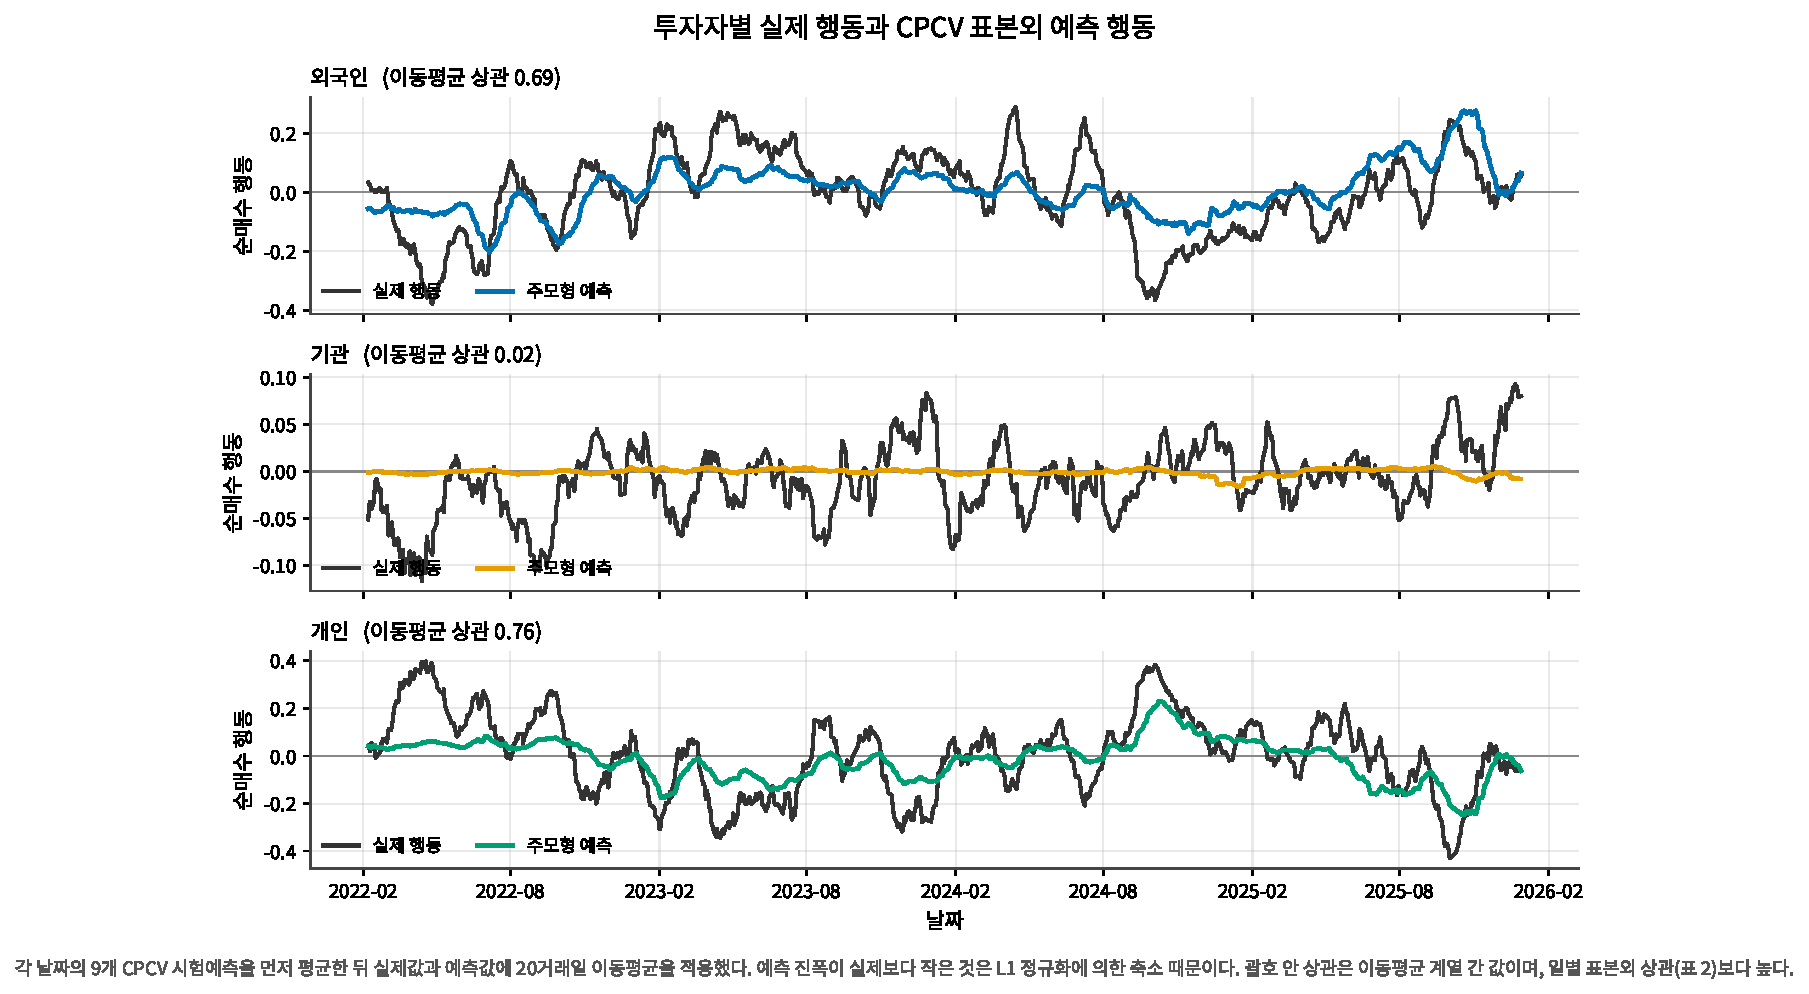
\includegraphics[width=\columnwidth]{../figures_v2/fig2_actual_vs_prediction.pdf}
  \caption{Actual and out-of-sample predicted net buying by investor type. The
  nine CPCV test predictions available for each date are averaged first, then a
  20-day moving average is applied to both the actual and the predicted series.
  Correlations in the panel titles are between the smoothed series and are not
  directly comparable to the daily out-of-sample correlations in
  Table~\ref{tab:performance}.}
  \Description{Three line charts overlaying actual net buying and model
  predictions over time for foreign, institutional and retail investors. In the
  institutional panel the prediction line is flat near zero.}
  \label{fig:prediction}
\end{figure}

Figure~\ref{fig:prediction} places actual and predicted net buying side by side
for the three types. Three things are immediately visible. First, for foreign
and retail investors the predicted series tracks the regime turns of the actual
series, with smoothed correlations of 0.69 and 0.76. Second, the predicted
amplitude is markedly smaller than the actual one, a consequence of coefficient
shrinkage under the $L_1$ penalty. Third, the institutional prediction is
essentially pinned to zero (0.02): the null reported in \S\ref{sec:null} appears
first in the prediction series rather than in a coefficient table.

\begin{table}[t]
  \caption{Out-of-sample performance under CPCV (mean $\pm$ s.d.\ over 45
  splits) and the persistence baseline}
  \label{tab:performance}
  \small
  \centering
  \begin{tabular}{@{}lccc@{}}
    \toprule
    Metric & Foreign & Institutional & Retail \\
    \midrule
    \multicolumn{4}{@{}l}{\emph{Main model}}\\
    Directional accuracy & $0.636\pm0.039$ & $0.542\pm0.038$ & $0.608\pm0.044$ \\
    Correlation          & $0.278\pm0.110$ & $0.068\pm0.064$ & $0.245\pm0.118$ \\
    MAE                  & $0.195\pm0.019$ & $0.094\pm0.008$ & $0.264\pm0.029$ \\
    RMSE                 & $0.246\pm0.021$ & $0.125\pm0.012$ & $0.318\pm0.030$ \\
    MAE / action s.d.    & $0.759$ & $0.756$ & $0.791$ \\
    Saturation rate      & $0.000$ & $0.000$ & $0.000$ \\
    \addlinespace
    \multicolumn{4}{@{}l}{\emph{Persistence baseline} ($a_{t+1}\leftarrow a_t$)}\\
    Directional accuracy & $\mathbf{0.642}$ & $\mathbf{0.547}$ & $\mathbf{0.616}$ \\
    Correlation          & $\mathbf{0.359}$ & $\mathbf{0.136}$ & $\mathbf{0.311}$ \\
    MAE                  & $0.223$ & $0.123$ & $0.299$ \\
    \addlinespace
    Action AR(1)         & $0.401$ & $0.149$ & $0.345$ \\
    \bottomrule
  \end{tabular}
\end{table}

\begin{figure}[t]
  \centering
  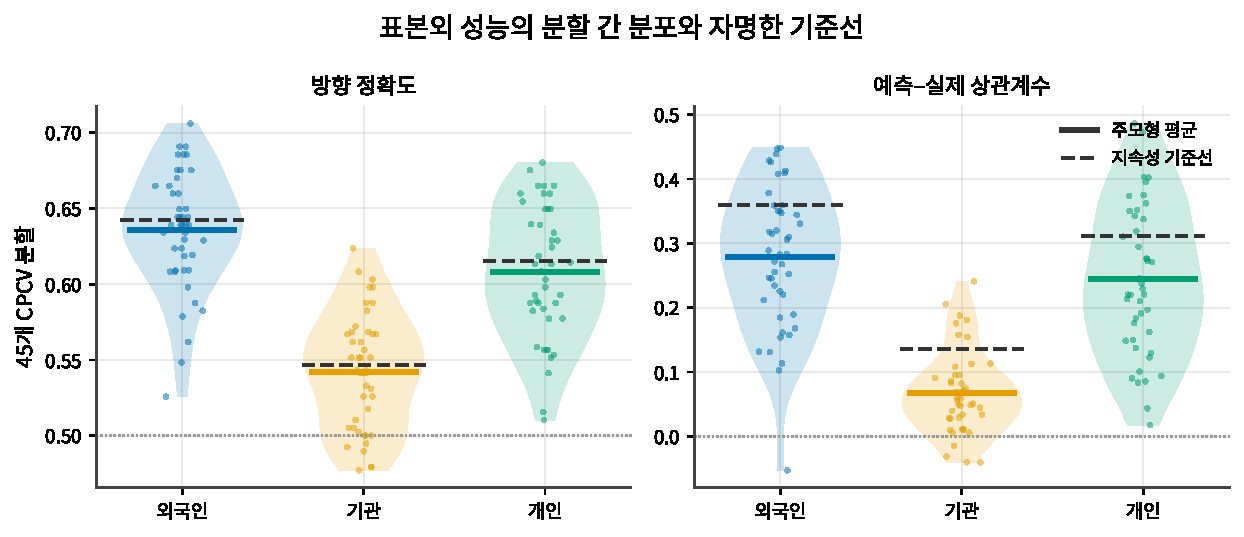
\includegraphics[width=\columnwidth]{../figures_v2/fig5_oos_performance.pdf}
  \caption{Split-level distribution of out-of-sample performance against a naive
  baseline. Solid lines are the main-model mean and dashed lines the persistence
  baseline. The dashed line lies above the solid line for all three types.}
  \Description{Two panels showing violin and point distributions of directional
  accuracy and correlation across 45 splits for the three investor types.}
  \label{fig:oos}
\end{figure}

Table~\ref{tab:performance} and Figure~\ref{fig:oos} reveal two things that
means alone conceal. First, dispersion across splits is large: the foreign
correlation ranges from $-0.05$ to $0.45$, so comparing types from a single
split is meaningless. Second, the naive persistence baseline outperforms the
main model on both directional accuracy and correlation. Since $a_t$ is
published after the day-$t$ close, this is an informationally feasible rule. The
main model leads only on MAE, and because that follows from shrinkage of the
predicted amplitude it cannot be read as an informational advantage.

The reason for the gap is clear. The action has first-order autocorrelation of
$0.401/0.149/0.345$, yet our reward feature set does not include the lagged own
action. Restricting the features to (F1)--(F3) was a design choice ensuring that
all three types share only features corresponding to independently established
behavioural regularities; it was not a design aimed at maximizing predictive
performance. We report this result openly in Table~\ref{tab:performance}.
Table~\ref{tab:performance} and Figure~\ref{fig:oos} are used to show that the
model has not merely fitted noise, not as evidence of predictive superiority.

Because the saturation rate is exactly zero for every type in every split, the
premise $|q|\le1$ of Proposition~\ref{prop:lasso} holds throughout the sample.
The estimator is therefore literally the Lasso of Equation~\eqref{eq:lasso}, and
performance does not rely on extreme $\pm1$ predictions.

\subsection{Recovered Rewards: A Mirror Image on the Momentum Axis}
\label{sec:beta}

\begin{figure*}[t]
  \centering
  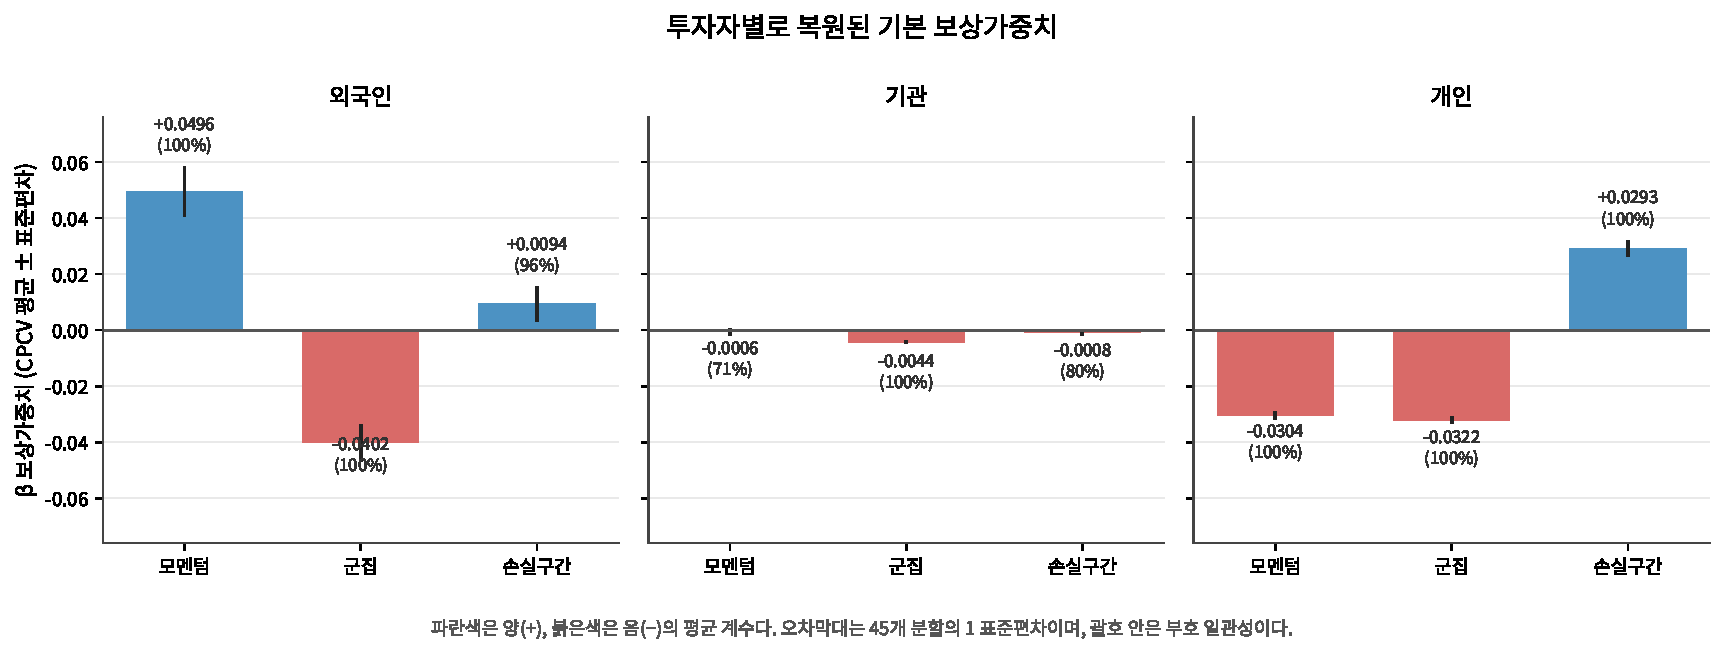
\includegraphics[width=\textwidth]{../figures_v2/fig1_reward_weights_bar.pdf}
  \caption{Recovered baseline reward weights $\beta$ by investor type. Blue bars
  are positive and red bars negative mean coefficients; error bars are one
  standard deviation across the 45 splits and the parenthesised figure is sign
  consistency.}
  \Description{Three bar charts giving momentum, herding and underwater
  coefficients for foreign, institutional and retail investors. Foreign momentum
  is positive, retail momentum negative, and the institutional bars are barely
  visible.}
  \label{fig:betabar}
\end{figure*}

\begin{figure*}[t]
  \centering
  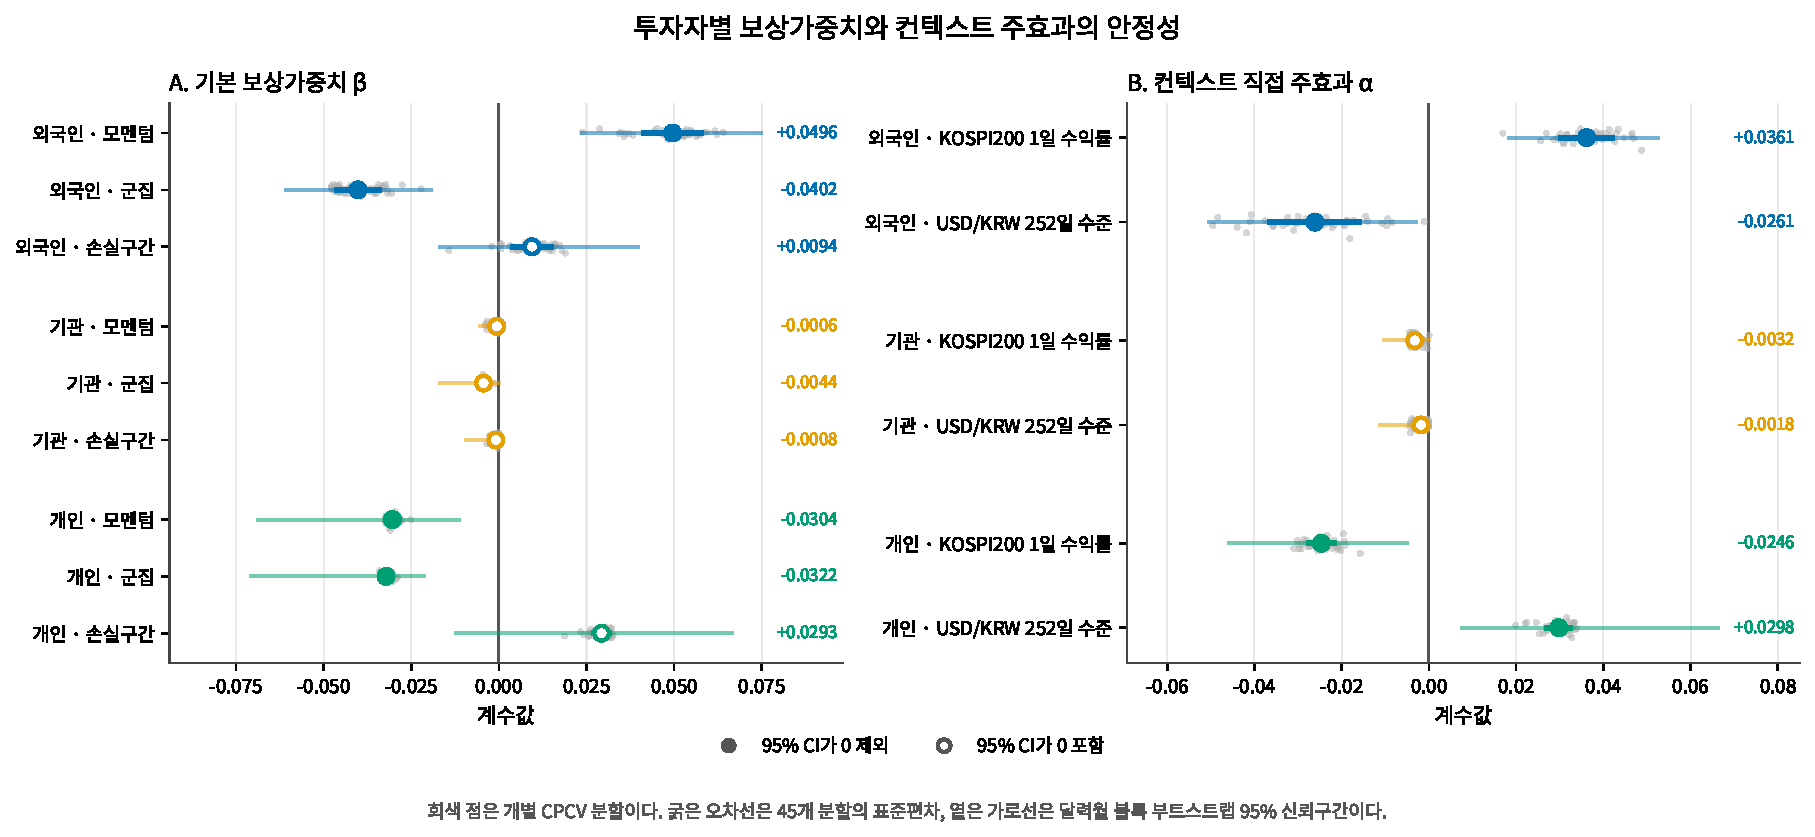
\includegraphics[width=\textwidth]{../figures_v2/fig3_beta_alpha_forest.pdf}
  \caption{Split-level stability of reward weights and context main effects.
  Grey dots are individual CPCV splits, thick error bars the standard deviation
  across the 45 splits, and light horizontal lines the 95\% calendar-month block
  bootstrap interval. Hollow markers denote terms whose interval contains zero.}
  \Description{Forest plots for baseline reward weights (panel A) and context
  main effects (panel B), showing per-split estimates and confidence intervals
  for each term.}
  \label{fig:forest}
\end{figure*}

Figure~\ref{fig:betabar} places the recovered baseline reward weights of the
three types side by side. Because all types received the same feature set and
the same model form and only their parameters were estimated separately, the
differences in bar height are entirely learned from the data.
Figure~\ref{fig:forest} unfolds the same $\beta$ together with the context main
effects $\alpha$ down to the split level.

\paragraph{The mirror image on the momentum axis}
The foreign momentum weight is $+0.0496$ and positive in all 45 splits, while
the retail weight is $-0.0304$ and negative in all 45 splits. In
Figure~\ref{fig:betabar} the two bars point in opposite directions across the
zero line, and in Figure~\ref{fig:forest} their bootstrap intervals do not
overlap and each excludes zero. Although the same feature set was estimated
independently for each type, the two types diverge in exactly opposite
directions on momentum: foreign investors appear as trend followers and retail
investors as contrarians, matching the sign expectations of prior
work~\cite{grinblatt2000investment,choe1999foreign}.

\paragraph{Herding}
The herding coefficient is negative in all 45 splits for all three types, and
the bootstrap intervals of the foreign ($-0.0402$) and retail ($-0.0322$)
coefficients also exclude zero. This result, however, does not separate a
behavioural interpretation from the market-clearing constraint. As
Figure~\ref{fig:crossinv} shows, the same-day correlation between types reaches
$-0.77$, so a substantial part of the negative herding coefficient may arise
mechanically. Because Equation~\eqref{eq:herd} uses a one-day lag the same-day
constraint does not apply directly, but it can propagate through the
autocorrelation of the action. We therefore restrict this result to the
descriptive statement that observed aggregate flow displays a negative
cross-type association, and do not extend it to the behavioural claim that each
type independently trades against the others.

\paragraph{Underwater}
The retail underwater weight is $+0.0293$ and positive in all 45 splits: buying
intensity rises on the following day when the traded price is below the
average-cost proxy, consistent with the reference-price dependence of the
disposition-effect literature~\cite{shefrin1985disposition,odean1998investors}.
The foreign coefficient shares the sign at $+0.0094$ (95.6\%) but is about a
third of the retail magnitude.

As Figure~\ref{fig:forest} shows, however, the underwater bootstrap interval
contains zero for all three types. The retail interval is
$[-0.0122,+0.0665]$: although the sign is 100\% consistent across the 45 splits,
it flips in 5.5\% of month-block resamples. This is exactly the situation
anticipated in \S\ref{sec:protocol}, where sign consistency understates
uncertainty because CPCV splits share observations. We therefore report that a
sign consistent with the disposition effect was observed, but do not claim it as
a statistically established result.

\subsection{Context Response: The Mirror Image Reappears}
\label{sec:alpha}

The mirror image observed on the momentum axis reappears in the context main
effects (panel B of Figure~\ref{fig:forest}). Foreign investors shift toward net
buying on days when the market rises ($+0.0361$) and toward net selling when the
won is weak ($-0.0261$), while retail investors do exactly the opposite on both
contexts ($-0.0246$ and $+0.0298$). All four coefficients keep their sign in all
45 splits and all four bootstrap intervals exclude zero. The two institutional
coefficients have sign consistency above 95\% but are about an eighth of the
foreign and retail magnitudes, and their intervals contain zero.

This mirror image requires the same interpretive reservation as the herding
coefficient. Given the $-0.772$ correlation in Figure~\ref{fig:crossinv}, two
types responding to context with opposite signs may in part reflect the
market-clearing constraint. We therefore present this as the descriptive fact
that the two types form opposite sides of order flow across market and exchange
rate conditions.

\paragraph{Interactions}
Of the twelve interaction coefficients, four keep their sign in all 45 splits:
foreign momentum $\times$ KOSPI200 ($-0.0139$), retail momentum $\times$ FX
($+0.0144$), retail herding $\times$ KOSPI200 ($-0.0080$) and retail
underwater $\times$ FX ($-0.0186$). Only the first and the last of these pass
the bootstrap. Since twelve coefficients were examined jointly, we present the
interactions as exploratory results only.

\subsection{Results of the Stability Protocol}
\label{sec:stability}

\paragraph{(V2) Calendar-month block bootstrap}
The light horizontal lines in Figure~\ref{fig:forest} give this result. The
bootstrap is a stricter criterion than CPCV sign consistency, and the outcome
splits three ways. First, the momentum mirror and the context mirror survive:
eight terms, comprising foreign and retail momentum, herding, and both context
main effects, all exclude zero. Second, the underwater weights do not survive.
Third, no institutional term excludes zero; all six institutional markers in
Figure~\ref{fig:forest} are hollow.

\begin{figure*}[t]
  \centering
  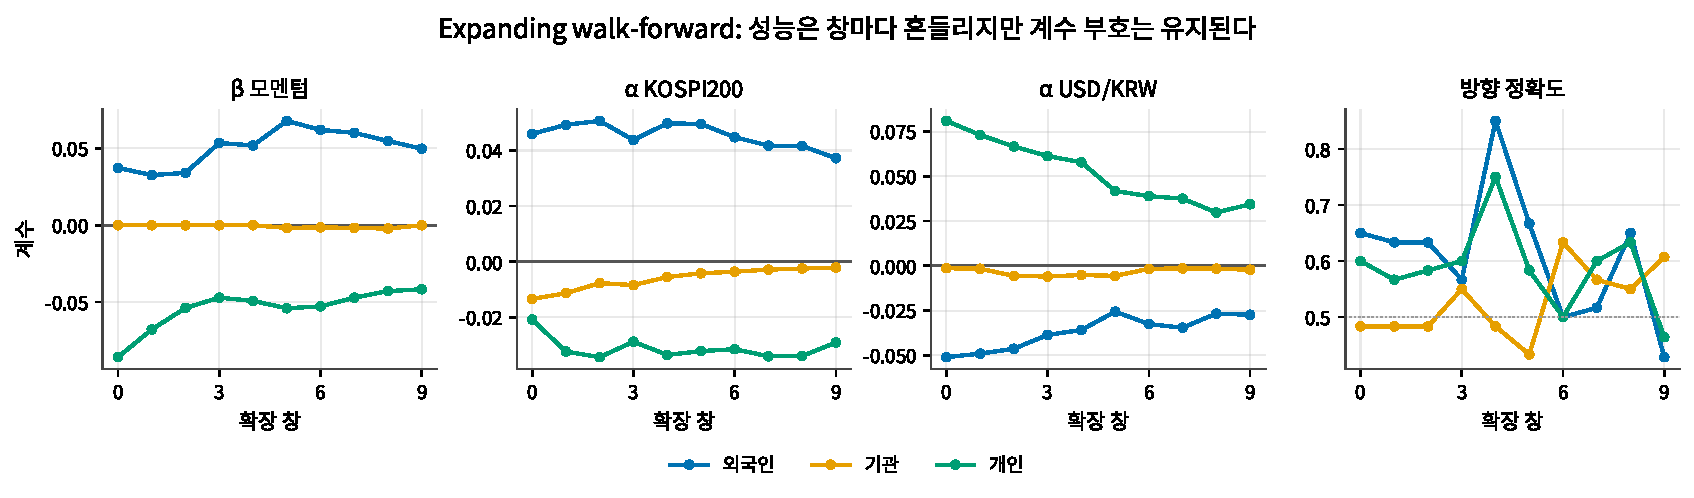
\includegraphics[width=\textwidth]{../figures_v2/fig6_walk_forward.pdf}
  \caption{Coefficient paths and directional accuracy over ten expanding
  walk-forward windows. Performance fluctuates from window to window while the
  coefficient signs hold.}
  \Description{Four line charts against the expanding-window index showing the
  momentum coefficient, the two context main effects, and directional accuracy
  for the three investor types.}
  \label{fig:walkforward}
\end{figure*}

\paragraph{(V3) Expanding walk-forward}
Figure~\ref{fig:walkforward} gives this result, and two things read at once.
Performance fluctuates sharply across windows: foreign directional accuracy
moves between 0.43 and 0.85, averaging $0.610\pm0.116$, and the correlation
falls to $0.131\pm0.162$, less than half the CPCV value of 0.278; retail falls
from 0.245 to 0.129. Because CPCV can place a test fold ahead of a training fold
while walk-forward cannot, we report this degradation as a generalization limit
arising from the temporal structure.

The coefficient paths, by contrast, do not fluctuate. The foreign momentum
coefficient is positive in all ten windows and the retail one negative in all
ten, and the two paths never cross. The same mirror image persists across all
windows for both context main effects, while the three institutional paths stay
pinned near zero. Performance moves with time; the direction of the recovered
preference does not.

\begin{figure*}[t]
  \centering
  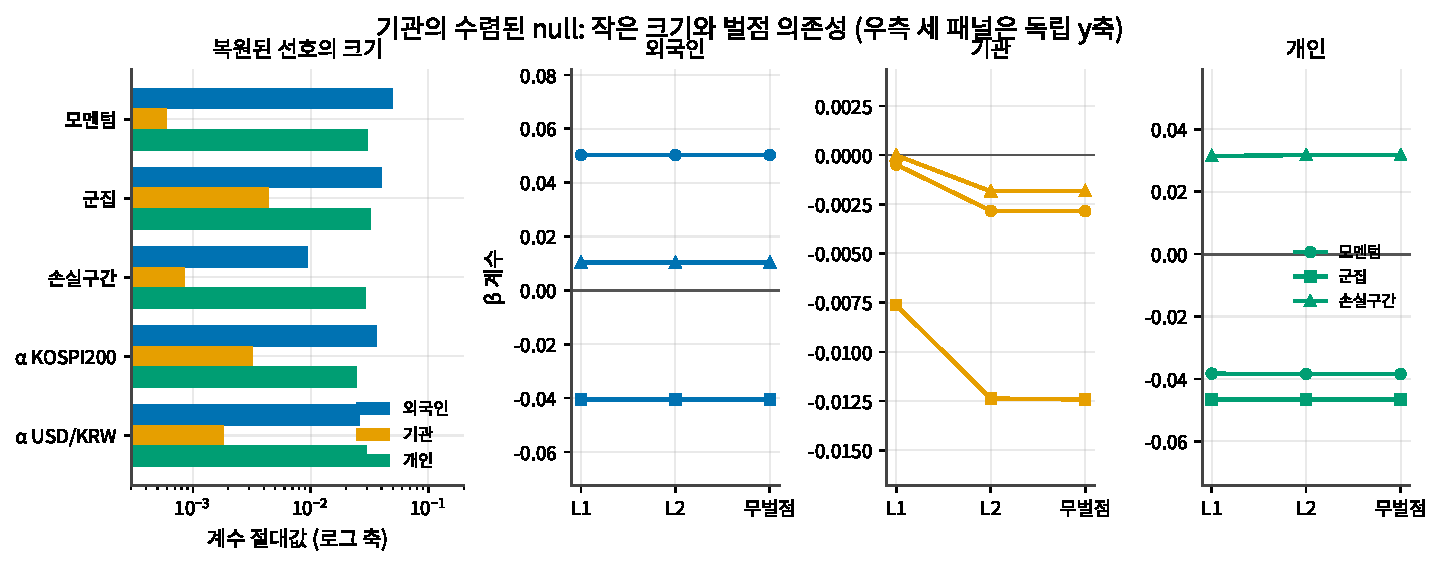
\includegraphics[width=\textwidth]{../figures_v2/fig7_institution_null.pdf}
  \caption{The converged institutional null. Left: magnitude of the recovered
  preferences on a logarithmic axis. Right: sensitivity to the regularization
  swap, with an independent $y$ axis in each of the three panels.}
  \Description{A logarithmic bar chart of coefficient magnitudes by type on the
  left, and three line charts of coefficients under L1, L2 and no penalty on the
  right.}
  \label{fig:null}
\end{figure*}

\paragraph{(V4) Regularization swap}
Figure~\ref{fig:null} gives this result. The foreign and retail coefficients are
effectively invariant to the choice of penalty, agreeing to four decimal places,
so the momentum mirror is not an artefact of the $L_1$ penalty. Only the
institutional coefficients move with the penalty (herding
$-0.0076\rightarrow-0.0124$, underwater $-0.0000\rightarrow-0.0018$), on a
$y$-axis range about one twentieth of that of the other two types. That the
coefficients depend on the choice of penalty means the data do not determine
their value.

\subsection{Institutional Investors: A Converged Null}
\label{sec:null}

For institutional order flow we find no preference that is stably identified at
daily frequency, and we report this as a finding rather than concealing it. The
evidence is fivefold and all of it is visible in the figures.

\begin{enumerate}
\item \textbf{Degenerate prediction.} In the middle panel of
Figure~\ref{fig:prediction} the institutional prediction stays on the zero line
while the actual series moves between $\pm0.1$.
\item \textbf{Magnitude.} In Figure~\ref{fig:betabar} the three institutional
bars are barely visible on the shared axis. Excluding herding, momentum is
$-0.0006$ and underwater $-0.0008$, about one fortieth of the other types.
\item \textbf{Uncertainty.} All six institutional markers in
Figure~\ref{fig:forest} are hollow.
\item \textbf{Penalty dependence.} In the middle right panel of
Figure~\ref{fig:null}, only the institutional coefficients move with the
penalty.
\item \textbf{Temporal instability.} In Figure~\ref{fig:walkforward} the
institutional paths hug the zero line; momentum sign consistency is 40\% of ten
windows and underwater 0\%.
\end{enumerate}

\begin{figure*}[t]
  \centering
  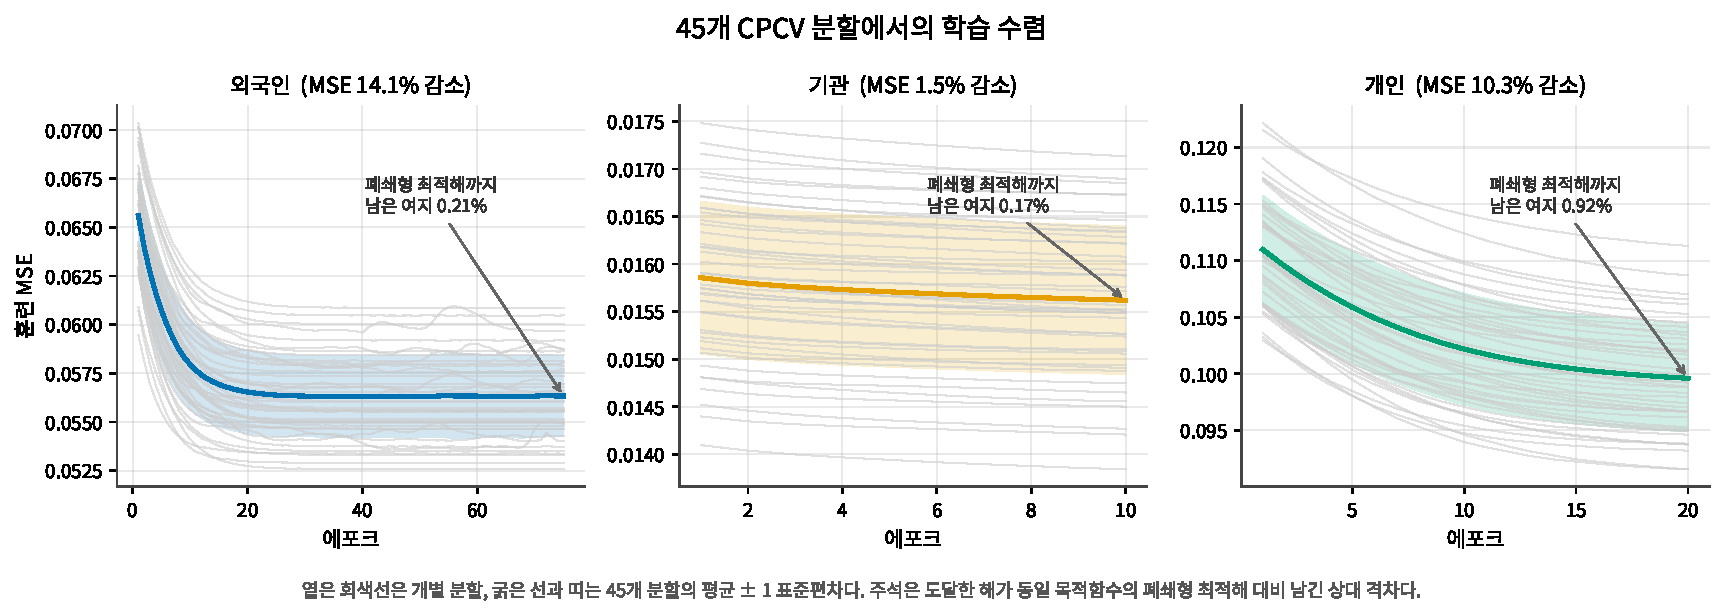
\includegraphics[width=\textwidth]{../figures_v2/fig4_training_convergence.pdf}
  \caption{Training convergence across the 45 CPCV splits. Light grey lines are
  individual splits; the thick line and band are the mean $\pm$ one standard
  deviation. The annotation gives the relative gap between the solution reached
  and the closed-form optimum of the same objective.}
  \Description{Three panels of training MSE against epoch for the three investor
  types; the institutional panel shows the smallest decrease.}
  \label{fig:convergence}
\end{figure*}

This null is not an optimization failure. Figure~\ref{fig:convergence} shows the
training curves across the 45 splits. The institutional training MSE falls by
only 1.5\% over the whole training run and the curve does not look visually
flat. That is not underfitting, however, but the fact that there is almost no
error left to remove. By Proposition~\ref{prop:lasso}, Equation~\eqref{eq:loss}
is convex with a unique global optimum, and comparing the solution reached with
the closed-form optimum of the same objective leaves an institutional gap of
only 0.17\% on average and 0.48\% at most (0.21\% for foreign and 0.92\% for
retail). All three types reach the attainable optimum; only for institutional
investors do the coefficients at that optimum sit near zero. The data do not
determine an institutional preference; it is not that the optimizer failed to
find one.

Economically the null reads naturally. The ``institutional'' category aggregates
pension funds, investment trusts, insurers, private funds, and securities firms,
so the flows of agents with different objective functions offset one another.
The one consistently negative herding coefficient is compatible with a shared
liquidity-provision role on the opposite side of the other types, but because
its bootstrap interval sits on the boundary we do not claim it.

\subsection{Construct Validity Check}
\label{sec:construct}

\begin{table}[t]
  \caption{Prior sign expectations and recovered results}
  \label{tab:construct}
  \small
  \begin{tabular}{@{}>{\raggedright\arraybackslash}p{0.26\columnwidth}
                  >{\raggedright\arraybackslash}p{0.14\columnwidth}
                  >{\raggedright\arraybackslash}p{0.24\columnwidth}
                  >{\raggedright\arraybackslash}p{0.20\columnwidth}@{}}
    \toprule
    Regularity & Expected & Recovered & Verdict \\
    \midrule
    Foreign trend trading~\cite{grinblatt2000investment,choe1999foreign}
      & $\beta^{mom}>0$ & $+0.0496$ (100\%, CI excl.\ 0) & matches \\
    Retail contrarian trading~\cite{grinblatt2000investment,kaniel2008individual}
      & $\beta^{mom}<0$ & $-0.0304$ (100\%, CI excl.\ 0) & matches \\
    Disposition effect~\cite{shefrin1985disposition,odean1998investors}
      & $\beta^{uw}>0$ & $+0.0293$ (100\%, CI incl.\ 0) & partial \\
    Institutional herding~\cite{lakonishok1992impact}
      & $\beta^{herd}>0$ & $-0.0044$ (100\%, CI incl.\ 0) & mismatch \\
    \bottomrule
  \end{tabular}
\end{table}

Table~\ref{tab:construct} reports the contrast. Although all three types
received the same features and the same model form and only their parameters
were estimated separately, the recovered signs agree with independently
established regularities and the two types diverge in opposite directions on
momentum. This is evidence of construct validity: the recovered reward is not an
arbitrary fit.

The mismatch arises because the measured object differs. Lakonishok et
al.~\cite{lakonishok1992impact} measure the extent to which agents \emph{within}
the institutional group move in the same direction, whereas
Equation~\eqref{eq:herd} measures whether institutions move with the previous
day's flow of the \emph{other two types}. Our result is therefore not a
refutation of that literature; testing within-type herding would require data on
institutional sub-categories.

\subsection{What This Study Does Not Claim}
\label{sec:notclaim}

As the final stage of the protocol we state explicitly what the results do not
support.

\begin{enumerate}
\item \textbf{Return predictability.} Our metrics are reproduction errors for
the direction and intensity of order flow and include no returns, Sharpe ratios,
or transaction costs. No trading rule follows from
Table~\ref{tab:performance}.

\item \textbf{Superior flow prediction.} As reported in
Table~\ref{tab:performance} and Figure~\ref{fig:oos}, the persistence baseline
beats the main model on directional accuracy and correlation. Our objective is
preference recovery on an interpretable common scale rather than predictive
performance, and the two objectives call for different feature sets. In a
preliminary check, adding the lagged own action as a fourth feature lifts the
model above the baseline (directional accuracy $0.646/0.569/0.629$) but reverses
the sign of the retail $\alpha^{KOSPI}$ and eliminates the underwater
coefficient. Some of the mirror images reported here are therefore not separable
from the autocorrelation of order flow.

\item \textbf{Causal effects.} The recovered weights are conditional
associations among standardized observed features. Because feature--context
correlations range from $-0.29$ to $0.22$ (Figure~\ref{fig:featcorr}), the
magnitude of any coefficient depends on the other terms being controlled for.

\item \textbf{A behavioural reading of the negative cross-type association.} The
herding coefficient and the mirrored context responses are not separable from
the market-clearing constraint (Figure~\ref{fig:crossinv}).

\item \textbf{A test of the disposition effect.} The retail underwater sign
agrees with the literature but does not pass the month-block bootstrap
(Figure~\ref{fig:forest}), and the average-cost proxy is built from aggregate
trades rather than account-level realized gains and holding periods.

\item \textbf{Generalization across stocks.} The single-stock design is a
control for isolating heterogeneity across types; extension to other stocks and
markets is untested.
\end{enumerate}

% =====================================================================
\appendix

\section{Supplementary Material}
\label{sec:appendix}

This appendix collects the supporting figures and tables referenced in the main
text. Figure~\ref{fig:saturation} verifies the premise of
Proposition~\ref{prop:lasso}, Figure~\ref{fig:featcorr} reports
feature--context correlations, and Figure~\ref{fig:crossinv} shows same-day
actions across types. Table~\ref{tab:interactions} lists the full set of
interaction coefficients presented as exploratory in the main text, and
Table~\ref{tab:convergence} reports the optimality check of the solution
reached.

\begin{figure}[htbp]
  \centering
  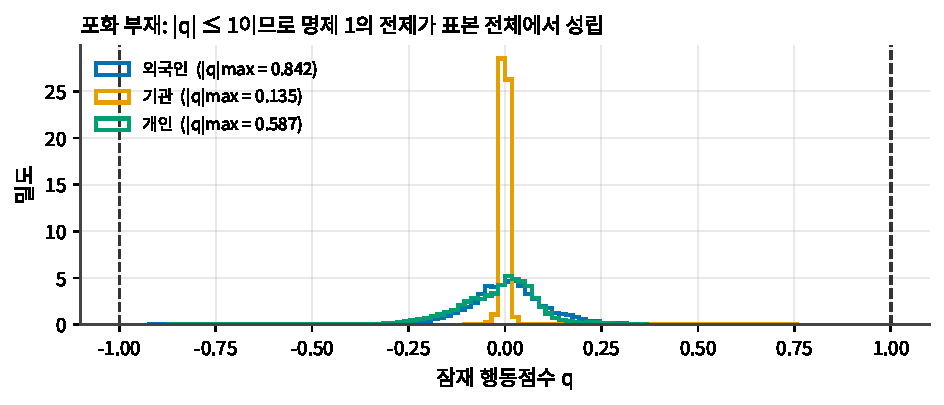
\includegraphics[width=\columnwidth]{../figures_v2/figA1_no_saturation.pdf}
  \caption{Distribution of the latent action score against the action bounds.
  Since $|q|\le1$, the premise of Proposition~\ref{prop:lasso} holds throughout
  the sample and the saturation rate is exactly zero in all 45 splits.}
  \Description{Histograms of the latent action score for the three types with
  the $\pm1$ bounds marked.}
  \label{fig:saturation}
\end{figure}

\begin{figure}[htbp]
  \centering
  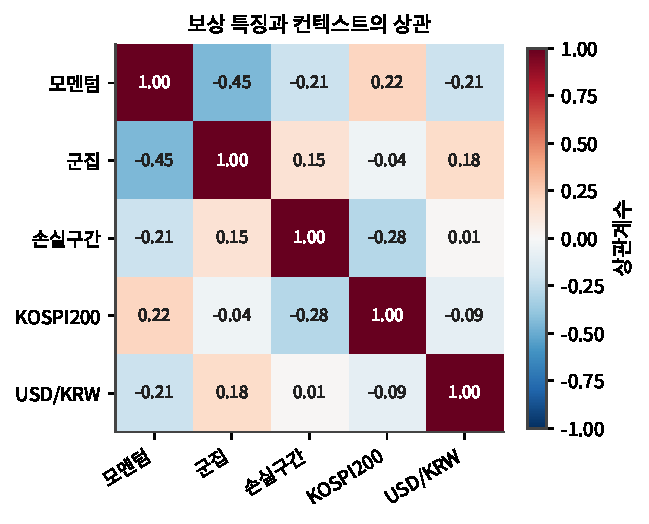
\includegraphics[width=\columnwidth]{../figures_v2/figA2_feature_correlation.pdf}
  \caption{Correlation matrix of reward features and contexts (foreign features,
  973 observations).}
  \Description{A heatmap showing correlation coefficients among five variables
  in colour and numerals.}
  \label{fig:featcorr}
\end{figure}

\begin{figure}[htbp]
  \centering
  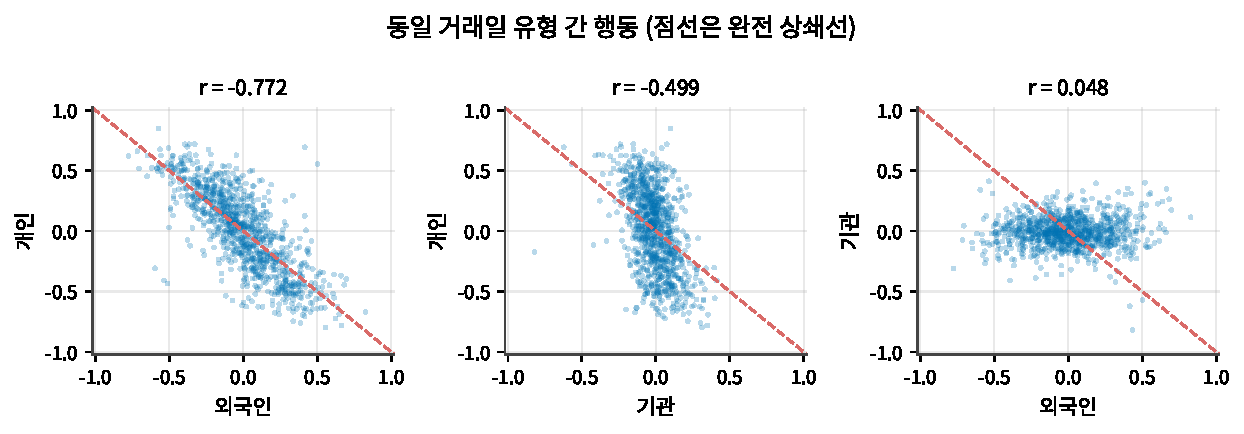
\includegraphics[width=\columnwidth]{../figures_v2/figA3_cross_investor_actions.pdf}
  \caption{Same-day actions across investor types. The dashed line marks perfect
  offset; foreign and retail actions cluster along it.}
  \Description{Three scatter plots of actions for each pair of investor types
  with the corresponding correlation coefficients.}
  \label{fig:crossinv}
\end{figure}

\begin{table}[htbp]
  \caption{Interaction coefficients $B$ (45 splits)}
  \label{tab:interactions}
  \small
  \centering
  \begin{tabular}{@{}llrrr@{}}
    \toprule
    Type & Feature $\times$ context & Mean & S.d. & Sign cons. \\
    \midrule
    Foreign & momentum $\times$ KOSPI200 & $-0.0139$ & $0.0052$ & 100.0\% \\
    Foreign & momentum $\times$ FX       & $-0.0030$ & $0.0057$ & 71.1\% \\
    Foreign & herding $\times$ KOSPI200  & $+0.0016$ & $0.0074$ & 66.7\% \\
    Foreign & herding $\times$ FX        & $+0.0037$ & $0.0073$ & 68.9\% \\
    Foreign & underwater $\times$ KOSPI200 & $-0.0062$ & $0.0040$ & 93.3\% \\
    Foreign & underwater $\times$ FX     & $-0.0075$ & $0.0076$ & 86.7\% \\
    \addlinespace
    Inst. & momentum $\times$ KOSPI200 & $-0.0001$ & $0.0005$ & 66.7\% \\
    Inst. & momentum $\times$ FX       & $+0.0003$ & $0.0006$ & 80.0\% \\
    Inst. & herding $\times$ KOSPI200  & $-0.0004$ & $0.0006$ & 86.7\% \\
    Inst. & herding $\times$ FX        & $+0.0012$ & $0.0012$ & 93.3\% \\
    Inst. & underwater $\times$ KOSPI200 & $+0.0028$ & $0.0012$ & 97.8\% \\
    Inst. & underwater $\times$ FX     & $+0.0007$ & $0.0008$ & 91.1\% \\
    \addlinespace
    Retail & momentum $\times$ KOSPI200 & $+0.0021$ & $0.0042$ & 80.0\% \\
    Retail & momentum $\times$ FX       & $+0.0144$ & $0.0045$ & 100.0\% \\
    Retail & herding $\times$ KOSPI200  & $-0.0080$ & $0.0046$ & 100.0\% \\
    Retail & herding $\times$ FX        & $+0.0092$ & $0.0081$ & 82.2\% \\
    Retail & underwater $\times$ KOSPI200 & $-0.0022$ & $0.0046$ & 66.7\% \\
    Retail & underwater $\times$ FX     & $-0.0186$ & $0.0046$ & 100.0\% \\
    \bottomrule
  \end{tabular}
\end{table}

\begin{table}[htbp]
  \caption{Optimality check of the solution reached (45 splits)}
  \label{tab:convergence}
  \small
  \centering
  \begin{tabular}{@{}lccc@{}}
    \toprule
    Type & MSE drop & Gap (\%) & Cosine \\
     & (training) & mean / max & mean / min \\
    \midrule
    Foreign & 14.1\% & $0.21/3.10$ & $0.994/0.948$ \\
    Inst.   & 1.5\%  & $0.17/0.48$ & $0.935/0.832$ \\
    Retail  & 10.3\% & $0.92/1.40$ & $0.894/0.833$ \\
    \bottomrule
  \end{tabular}
\end{table}

%  Required packages: booktabs, graphicx, amsmath, array, url
%  Figure path: ../figures_v2/  (output of scripts/make_paper_figures.py)
%  Additional references: merge paper-refs-additional.bib
% =====================================================================

\section{Method}
\label{sec:method}

\subsection{Setup: Symmetric Estimation}
\label{sec:setup}

Let the set of investor types be
$\mathcal{I}=\{\text{foreign},\text{institutional},\text{retail}\}$. Each type is
treated as an agent whose observed daily order flow reveals a latent reward
defined over interpretable market state features.

\paragraph{Continuous action}
Writing $V^{buy}_{i,t}$ and $V^{sell}_{i,t}$ for the daily gross buy and gross
sell value of type $i$, we define the action as
\begin{equation}
u_{i,t}=\frac{V^{buy}_{i,t}-V^{sell}_{i,t}}
             {V^{buy}_{i,t}+V^{sell}_{i,t}}\in[-1,1].
\label{eq:action}
\end{equation}
Because the denominator is the type's own gross turnover rather than
market-wide turnover, $u_{i,t}$ measures whether buying or selling dominated
\emph{within} that type, giving a common scale that is unaffected by
differences in trading size across types. Using a continuous intensity rather
than a binary buy/sell label preserves the magnitude information that
dichotomization discards.

\paragraph{Symmetry}
All three types receive the same state features $x_{i,t}\in\mathbb{R}^{3}$, the
same market context $C_t\in\mathbb{R}^{2}$, and the same model form. No type is
assigned a different feature a priori; only the parameters
$\theta_i=(\beta_i,B_i,\alpha_i)$ are estimated separately on each type's own
data. Any difference that appears in the results is therefore learned from the
data rather than imposed by design, and this symmetry is what licenses direct
comparison of coefficients across types.

\paragraph{Timing}
The training sample is $(x_{i,t},C_t,a_{i,t+1})$ with $a_{i,t+1}=u_{i,t+1}$. A
state built from day-$t$ closing prices and order flow explains day-$t+1$
behaviour, so no future trade enters the features. Momentum and underwater use
day-$t$ information while the herding feature uses day $t-1$. Since the target
is day-$t+1$ behaviour, day-$t$ information is also available; the extra lag on
herding is therefore not an information constraint but a design choice that
keeps the same-day accounting offset between types out of the predictor set
(Figure~\ref{fig:crossinv}).

\subsection{Reward Features}
\label{sec:features}

All three features are standardized using statistics fitted on the training
indices of each validation split only. Every coefficient reported below is
therefore read as the effect of a one-standard-deviation move of that feature
within the training window.

\paragraph{(F1) Medium-term momentum}
With adjusted (or fallback) closing price $P_t$,
\begin{equation}
x^{mom}_{i,t}=\log\!\left(\frac{P_t}{P_{t-20}}\right).
\label{eq:momentum}
\end{equation}
Twenty trading days is a pre-specified window of roughly one month, chosen to
damp daily price noise while still expressing a medium-term trend linked to
next-day behaviour. It is a design value for interpretability, not a value tuned
on the data. A positive coefficient indicates trend following and a negative one
contrarian trading; the sign expectation follows prior work on type-specific
momentum trading~\cite{grinblatt2000investment,choe1999foreign}.

\paragraph{(F2) Herding}
The cross-sectional average of the previous day's actions of the two types other
than $i$:
\begin{equation}
x^{herd}_{i,t}=\frac{u_{j,t-1}+u_{k,t-1}}{2},\qquad j,k\neq i.
\label{eq:herd}
\end{equation}
Note that this is an average across the two other types at one point in time,
not a time average. A 20-day moving average would measure a month of cumulative
flow pressure rather than an immediate response, so we focus on the previous
day. A positive coefficient means moving with the previous day's direction of
the other types, a negative one means moving against it. The sign expectation
follows the institutional herding
literature~\cite{lakonishok1992impact}; note however that this literature
measures herding \emph{within} the institutional group, whereas
Equation~\eqref{eq:herd} measures a relation \emph{between} types
(\S\ref{sec:construct}).

\paragraph{(F3) Underwater gap relative to average cost}
With a per-type average-cost proxy $\bar P_{i,t}$ and the day's gross-trade VWAP
$P^{vwap}_{i,t}$,
\begin{equation}
x^{uw}_{i,t}=\max\!\left(
\frac{\bar P_{i,t}-P^{vwap}_{i,t}}{\bar P_{i,t}},\,0\right).
\label{eq:underwater}
\end{equation}
Truncation at zero makes the feature active only when the traded price sits
below the average-cost proxy, so the variable is reference-point dependent by
construction. The average cost is obtained by recursively updating an effective
inventory from gross buy and sell quantities and values: the previous day's
inventory is multiplied by a forgetting factor $\rho=0.98$ to damp the influence
of old trades, and sales do not change the average cost of the remaining
position. With $\rho=0.98$ the half-life is about 34 trading days and roughly
66.8\% remains after 20, so the feature emphasises the trading memory of the
past one to two months; this value was also not tuned on the data. A positive
coefficient means stronger next-day buying below the average cost, and the sign
expectation follows the disposition-effect
literature~\cite{shefrin1985disposition,odean1998investors}.

The proxy is constructed from aggregate flow rather than actual account
holdings. Buys and sells executed by different accounts within the same type
net out, so the notion of a ``representative investor's average cost'' is itself
an approximation. The coefficient on $x^{uw}$ therefore cannot be read as a
direct test of the disposition effect.

\subsection{Market Context}
\label{sec:context}

The context consists of two variables: (C1) the one-day KOSPI200 return $r_t$,
and (C2) the KRW/USD exchange rate level
\begin{equation}
z_t=\frac{\log e_t-\mu_{t-1,252}}{\sigma_{t-1,252}},
\label{eq:fxcontext}
\end{equation}
where the current rate is used but the mean and standard deviation are computed
only through $t-1$ over 252 trading days. Both contexts are likewise
re-standardized on the training indices of each split, so their coefficients
read as the effect of a one-standard-deviation move within the training window.

Context and reward features are not independent. Because Samsung Electronics
carries a large weight in the KOSPI200, stock momentum overlaps with the market
return, and feature--context correlations range from $-0.29$ to $0.22$
(Figure~\ref{fig:featcorr}). Individual coefficients are therefore conditional
associations given the other terms and should not be read as causal magnitudes
in isolation.

\subsection{Myopic Reward, Policy, and the Reduction to Lasso}
\label{sec:model}

\paragraph{Latent action score}
Define the action score of type $i$ at time $t$ as
\begin{equation}
q_{i,t}=(\beta_i+B_iC_t)^{\top}x_{i,t}+\alpha_i^{\top}C_t,
\label{eq:score}
\end{equation}
where $\beta_i\in\mathbb{R}^{3}$ is the baseline reward weight at average
context, $B_i\in\mathbb{R}^{3\times 2}$ the feature--context interaction, and
$\alpha_i\in\mathbb{R}^{2}$ the direct context main effect. The $\alpha$ term is
a level effect that shifts behaviour even when the stock features are at their
means; the $B$ term is a slope effect that changes sensitivity to each feature
across market conditions. Including interaction terms while omitting the
lower-order term $C_t$ is a standard specification error, so the inclusion of
$\alpha$ is required by the specification rather than something to be justified
empirically.

\paragraph{Myopic concave reward}
The one-step reward for a continuous action $a$ is
\begin{equation}
R_i(x,C,a)=q_{i,t}\,a-\frac{\kappa}{2}a^{2}.
\label{eq:reward}
\end{equation}
The quadratic term imposes a symmetric cost on large net buying and net selling
and makes the reward concave in the action, which permits an interior solution.
Without it, maximizing over $[-1,1]$ would return $\pm1$ almost always depending
only on the sign of $q$, and the \emph{intensity} of behaviour could not be
reproduced. Maximizing Equation~\eqref{eq:reward} over $a$ yields the closed-form
policy
\begin{equation}
a^{*}_{i,t+1}=\mathrm{clip}\!\left(\frac{q_{i,t}}{\kappa},-1,1\right).
\label{eq:policy}
\end{equation}
The curvature $\kappa$ is fixed at one for identification. With $\kappa=2$ the
same $q$ would halve the action size, but re-estimation would double the
coefficients of $q$ and reproduce the same behaviour; $\kappa=1$ therefore fixes
the units of the reward and the coefficients rather than asserting that the
empirical curvature equals one.

\paragraph{Estimation}
The training objective for each type on its training set $\mathcal{D}_i$ is
\begin{equation}
\min_{\theta_i}\ \frac{1}{|\mathcal{D}_i|}
\sum_{t\in\mathcal{D}_i}\bigl(a^{*}_{i,t+1}-a_{i,t+1}\bigr)^{2}
+\lambda_i\lVert\theta_i\rVert_1,
\label{eq:loss}
\end{equation}
optimized independently per type with Adam~\cite{kingma2015adam}.

\begin{proposition}[Reduction to Lasso]
\label{prop:lasso}
Let
$z_{i,t}=[\,x_{i,t};\ \mathrm{vec}(x_{i,t}C_t^{\top});\ C_t\,]\in\mathbb{R}^{11}$
and $\theta_i=[\,\beta_i;\ \mathrm{vec}(B_i);\ \alpha_i\,]$, so that
Equation~\eqref{eq:score} reads $q_{i,t}=\theta_i^{\top}z_{i,t}$. If
$|q_{i,t}|\le 1$ throughout the training sample, the clip in
Equation~\eqref{eq:policy} never binds, $a^{*}=q$, and
Equation~\eqref{eq:loss} becomes
\begin{equation}
\min_{\theta_i}\ \frac{1}{|\mathcal{D}_i|}
\sum_{t}\bigl(\theta_i^{\top}z_{i,t}-a_{i,t+1}\bigr)^{2}
+\lambda_i\lVert\theta_i\rVert_1,
\label{eq:lasso}
\end{equation}
which is exactly an $L_1$-penalized (Lasso) regression of next-day net-buying
intensity on the expanded state feature $z$.
\end{proposition}

Under a myopic concave reward with $\kappa=1$, ``recovering a preference'' and
``regressing order flow'' are therefore numerically indistinguishable.
Figure~\ref{fig:saturation} shows that the premise of
Proposition~\ref{prop:lasso} in fact holds in our sample: for all three types the
distribution of the latent action score sits far inside the action bounds
$\pm1$ (the maximum $|q|$ is 0.842 for foreign, 0.587 for retail and 0.135 for
institutional investors), and the saturation rate is exactly zero in all 45
splits.

\paragraph{Why we do not hide the reduction}
This coincidence is not a weakness of the method but a logical consequence of
the myopia assumption. If the agent looks only one step ahead, today's action
does not affect anything beyond tomorrow, so there is no future to look toward
and \emph{what the agent wants} (the reward) collapses onto \emph{what the agent
does} (the policy). Applying the stochastic policy of maximum-entropy
IRL~\cite{ziebart2008maximum}, $\pi(a\mid x,C)\propto\exp(R/\tau)$, to
Equation~\eqref{eq:reward} makes $\pi$ a truncated normal with mean $q$ and
variance $\tau$, whose maximum-likelihood point estimate coincides with
Equation~\eqref{eq:lasso}. The reduction is thus a property of the myopic,
quadratic-reward setting in general, not an artefact of one implementation.

The distinctive value of the inverse reinforcement learning formulation lies in
the extension path. Once state dynamics and multi-period value are introduced,
the reward separates from the policy and leads to a structural recovery that
regression cannot reach. This paper is the first step on that path, and it adds
interpretation and validation on top of an explicitly stated set of conditions.

\subsection{Validation Protocol}
\label{sec:protocol}

Rather than stopping at the sign and magnitude of the recovered coefficients, we
apply four stages.

\begin{description}
\item[(V1) Out-of-sample stability under CPCV] We use combinatorial purged
cross-validation~\cite{lopez2018advances} with ten temporal folds of which two
serve as test folds, giving $\binom{10}{2}=45$ splits, a one-day purge and a
five-day embargo between training and test, and all standardization fitted on
training indices only. We report the fraction of splits in which the dominant
sign appears (sign consistency), but because the splits share observations we
interpret sign consistency only as a stability indicator, never as an
independent-sample $p$-value.

\item[(V2) Calendar-month block bootstrap] To address the fact that sign
consistency is not a test, we partition the sample into calendar-month blocks,
resample months with replacement, and re-estimate 1{,}000 times to obtain 95\%
confidence intervals. Month blocks preserve the autocorrelation of daily flow
and within-month patterns inside each block.

\item[(V3) Expanding walk-forward] Because CPCV can place a test fold before a
training fold, we add a validation that strictly respects the arrow of time. We
train on the first 400 observations, predict the next 60 trading days after a
five-day purge, and repeat while expanding the training window by 60 trading
days, for ten windows in total.

\item[(V4) Regularization swap] To confirm that the results are not an artefact
of the $L_1$ penalty, we re-run the same protocol with an $L_2$ penalty and with
no penalty, and compare coefficient signs.
\end{description}

\paragraph{Metrics}
Magnitude error is measured by MAE and RMSE, and directional reproduction by
directional accuracy, the fraction of days with
$\mathrm{sign}(a^{*})=\mathrm{sign}(a)$. We also report the Pearson correlation
between actual and predicted actions and the saturation rate, the fraction with
$|a^{*}|=1$. Because action standard deviations differ across types, absolute
MAE and RMSE are not compared across types but interpreted within each type, and
we report errors normalized by the action standard deviation alongside them. As
a reference we also report a persistence rule that predicts the previous day's
own action (\S\ref{sec:notclaim}).

\paragraph{Construct validity check}
We contrast the recovered signs with expectations derived from independently
established behavioural-finance regularities (\S\ref{sec:construct}). This is a
comparison against sign expectations fixed in advance, not a post hoc
interpretation.

% =====================================================================
\section{Experiments}
\label{sec:experiments}

\subsection{Data and Setup}
\label{sec:data}

The raw data are daily records for Samsung Electronics (005930) and include
prices, trading value, gross buy and sell values and quantities by investor
type, the KRW/USD exchange rate, and KOSPI200 returns. Among the observations
for which the 252-day exchange-rate history, the 20-day momentum, and the next
day's action can all be computed, we use the most recent 973 rows. State dates
run from 6 January 2022 to 29 December 2025, with the last state targeting the
action of 30 December 2025.

The single-stock design is not a limitation of the sample but a controlled
demonstration setting that isolates preference heterogeneity across types
without cross-stock confounding. Because stock fixed effects, liquidity
differences, and index-inclusion effects do not intervene, differences in
coefficients across types can be attributed to learning rather than design.

\begin{table}[t]
  \caption{Data and estimation setup}
  \label{tab:setup}
  \small
  \begin{tabular}{@{}>{\raggedright\arraybackslash}p{0.30\columnwidth}
                  >{\raggedright\arraybackslash}p{0.62\columnwidth}@{}}
    \toprule
    Item & Setting \\
    \midrule
    Sample & 973 trading days, 2022-01-06--2025-12-29 \\
    Types & foreign, institutional, retail (symmetric estimation) \\
    Reward features & momentum (20d), herding (1d lag), underwater ($\rho=0.98$) \\
    Contexts & KOSPI200 1d return, USD/KRW 252d level $z$ \\
    Parameters per type & 11 ($\beta$ 3, $B$ 6, $\alpha$ 2) \\
    Common settings & seed 42, CPU, $\kappa=1$, train-only scaling \\
    Foreign & 75 epochs, batch 256, lr 0.001, $\lambda=0$ \\
    Institutional & 10 epochs, batch 2048, lr 0.0005, $\lambda=0.01$ \\
    Retail & 20 epochs, batch 512, lr 0.001, $\lambda=0.0003$ \\
    Validation & CPCV 10 folds, 2 test folds, purge 1, embargo 5, 45 splits \\
    Stability & month-block bootstrap 1{,}000, walk-forward 10 windows, penalty swap \\
    \bottomrule
  \end{tabular}
\end{table}

Mean actions are $-0.0063$ for foreign, $-0.0100$ for institutional and
$0.0035$ for retail investors, all close to zero, but standard deviations differ
markedly: retail is largest at 0.334 and institutional smallest at 0.125.
First-order autocorrelations are 0.401, 0.149 and 0.345 respectively.

Same-day actions across types are strongly negatively related
(Figure~\ref{fig:crossinv}). The foreign--retail correlation is $-0.772$ and the
institutional--retail correlation is $-0.499$, reflecting the market-clearing
constraint that one type's buying must appear as another's selling. This fact is
used again to bound the interpretation in \S\ref{sec:beta} and
\S\ref{sec:alpha}.

\subsection{Out-of-Sample Behaviour Reproduction}
\label{sec:oos}

\begin{figure}[t]
  \centering
  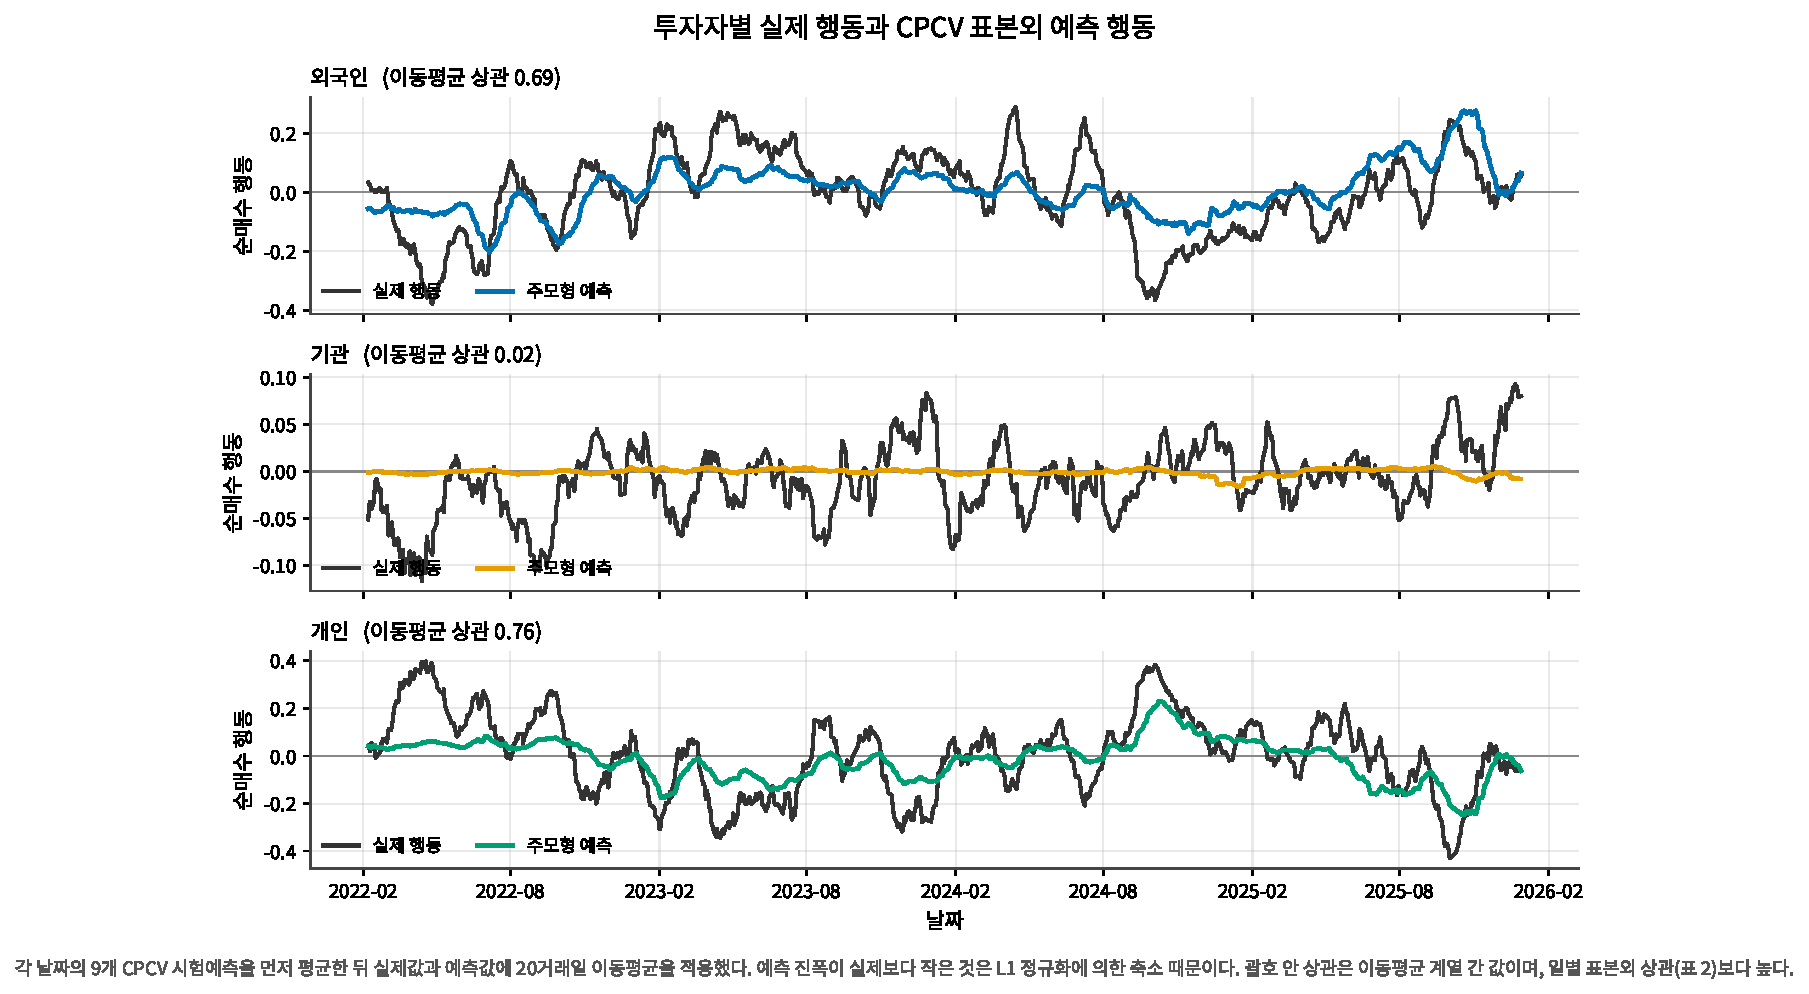
\includegraphics[width=\columnwidth]{../figures_v2/fig2_actual_vs_prediction.pdf}
  \caption{Actual and out-of-sample predicted net buying by investor type. The
  nine CPCV test predictions available for each date are averaged first, then a
  20-day moving average is applied to both the actual and the predicted series.
  Correlations in the panel titles are between the smoothed series and are not
  directly comparable to the daily out-of-sample correlations in
  Table~\ref{tab:performance}.}
  \Description{Three line charts overlaying actual net buying and model
  predictions over time for foreign, institutional and retail investors. In the
  institutional panel the prediction line is flat near zero.}
  \label{fig:prediction}
\end{figure}

Figure~\ref{fig:prediction} places actual and predicted net buying side by side
for the three types. Three things are immediately visible. First, for foreign
and retail investors the predicted series tracks the regime turns of the actual
series, with smoothed correlations of 0.69 and 0.76. Second, the predicted
amplitude is markedly smaller than the actual one, a consequence of coefficient
shrinkage under the $L_1$ penalty. Third, the institutional prediction is
essentially pinned to zero (0.02): the null reported in \S\ref{sec:null} appears
first in the prediction series rather than in a coefficient table.

\begin{table}[t]
  \caption{Out-of-sample performance under CPCV (mean $\pm$ s.d.\ over 45
  splits) and the persistence baseline}
  \label{tab:performance}
  \small
  \centering
  \begin{tabular}{@{}lccc@{}}
    \toprule
    Metric & Foreign & Institutional & Retail \\
    \midrule
    \multicolumn{4}{@{}l}{\emph{Main model}}\\
    Directional accuracy & $0.636\pm0.039$ & $0.542\pm0.038$ & $0.608\pm0.044$ \\
    Correlation          & $0.278\pm0.110$ & $0.068\pm0.064$ & $0.245\pm0.118$ \\
    MAE                  & $0.195\pm0.019$ & $0.094\pm0.008$ & $0.264\pm0.029$ \\
    RMSE                 & $0.246\pm0.021$ & $0.125\pm0.012$ & $0.318\pm0.030$ \\
    MAE / action s.d.    & $0.759$ & $0.756$ & $0.791$ \\
    Saturation rate      & $0.000$ & $0.000$ & $0.000$ \\
    \addlinespace
    \multicolumn{4}{@{}l}{\emph{Persistence baseline} ($a_{t+1}\leftarrow a_t$)}\\
    Directional accuracy & $\mathbf{0.642}$ & $\mathbf{0.547}$ & $\mathbf{0.616}$ \\
    Correlation          & $\mathbf{0.359}$ & $\mathbf{0.136}$ & $\mathbf{0.311}$ \\
    MAE                  & $0.223$ & $0.123$ & $0.299$ \\
    \addlinespace
    Action AR(1)         & $0.401$ & $0.149$ & $0.345$ \\
    \bottomrule
  \end{tabular}
\end{table}

\begin{figure}[t]
  \centering
  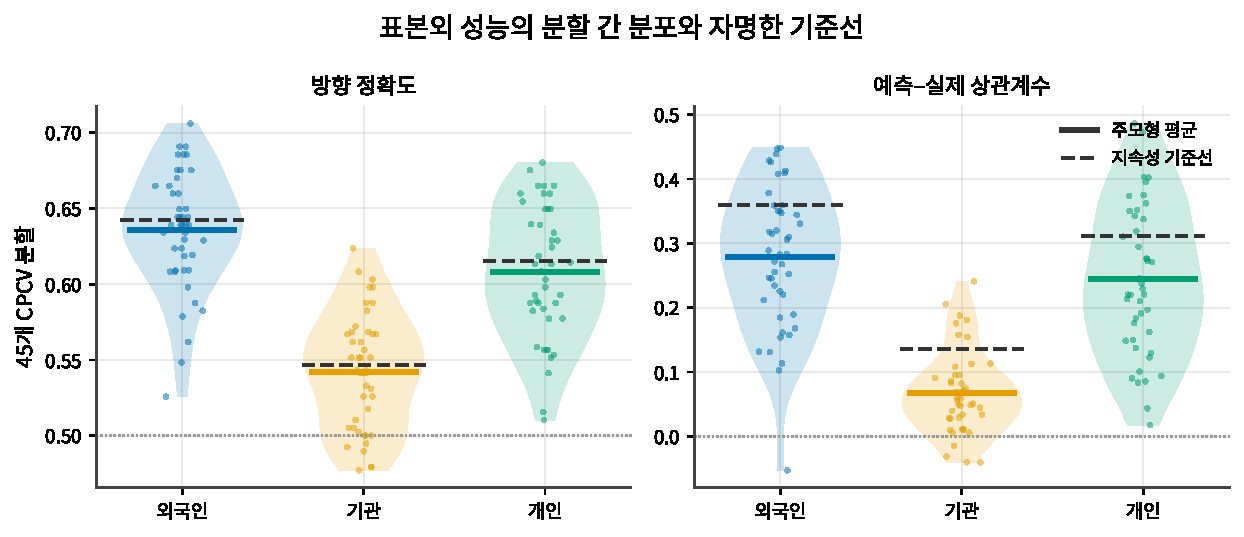
\includegraphics[width=\columnwidth]{../figures_v2/fig5_oos_performance.pdf}
  \caption{Split-level distribution of out-of-sample performance against a naive
  baseline. Solid lines are the main-model mean and dashed lines the persistence
  baseline. The dashed line lies above the solid line for all three types.}
  \Description{Two panels showing violin and point distributions of directional
  accuracy and correlation across 45 splits for the three investor types.}
  \label{fig:oos}
\end{figure}

Table~\ref{tab:performance} and Figure~\ref{fig:oos} reveal two things that
means alone conceal. First, dispersion across splits is large: the foreign
correlation ranges from $-0.05$ to $0.45$, so comparing types from a single
split is meaningless. Second, the naive persistence baseline outperforms the
main model on both directional accuracy and correlation. Since $a_t$ is
published after the day-$t$ close, this is an informationally feasible rule. The
main model leads only on MAE, and because that follows from shrinkage of the
predicted amplitude it cannot be read as an informational advantage.

The reason for the gap is clear. The action has first-order autocorrelation of
$0.401/0.149/0.345$, yet our reward feature set does not include the lagged own
action. Restricting the features to (F1)--(F3) was a design choice ensuring that
all three types share only features corresponding to independently established
behavioural regularities; it was not a design aimed at maximizing predictive
performance. We report this result openly in Table~\ref{tab:performance}.
Table~\ref{tab:performance} and Figure~\ref{fig:oos} are used to show that the
model has not merely fitted noise, not as evidence of predictive superiority.

Because the saturation rate is exactly zero for every type in every split, the
premise $|q|\le1$ of Proposition~\ref{prop:lasso} holds throughout the sample.
The estimator is therefore literally the Lasso of Equation~\eqref{eq:lasso}, and
performance does not rely on extreme $\pm1$ predictions.

\subsection{Recovered Rewards: A Mirror Image on the Momentum Axis}
\label{sec:beta}

\begin{figure*}[t]
  \centering
  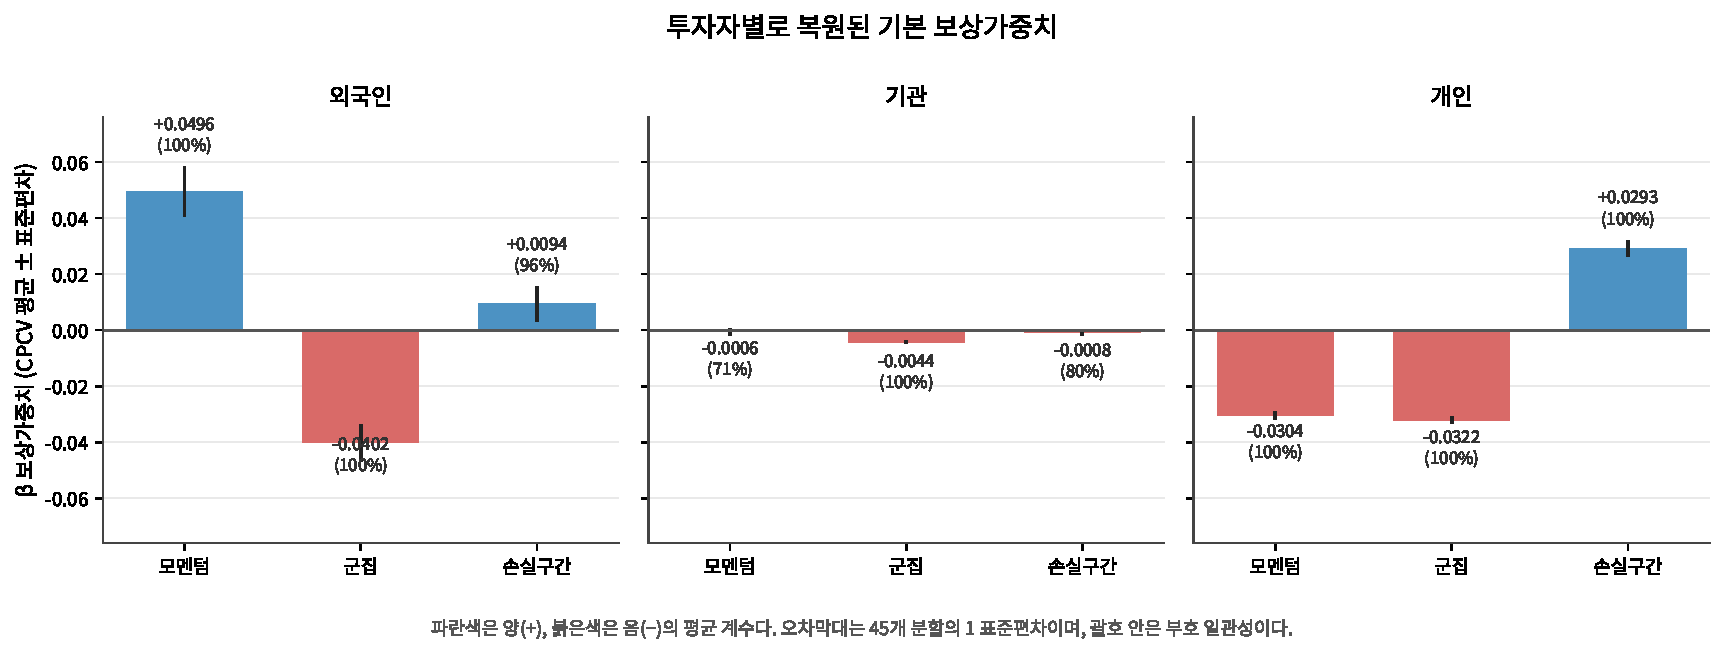
\includegraphics[width=\textwidth]{../figures_v2/fig1_reward_weights_bar.pdf}
  \caption{Recovered baseline reward weights $\beta$ by investor type. Blue bars
  are positive and red bars negative mean coefficients; error bars are one
  standard deviation across the 45 splits and the parenthesised figure is sign
  consistency.}
  \Description{Three bar charts giving momentum, herding and underwater
  coefficients for foreign, institutional and retail investors. Foreign momentum
  is positive, retail momentum negative, and the institutional bars are barely
  visible.}
  \label{fig:betabar}
\end{figure*}

\begin{figure*}[t]
  \centering
  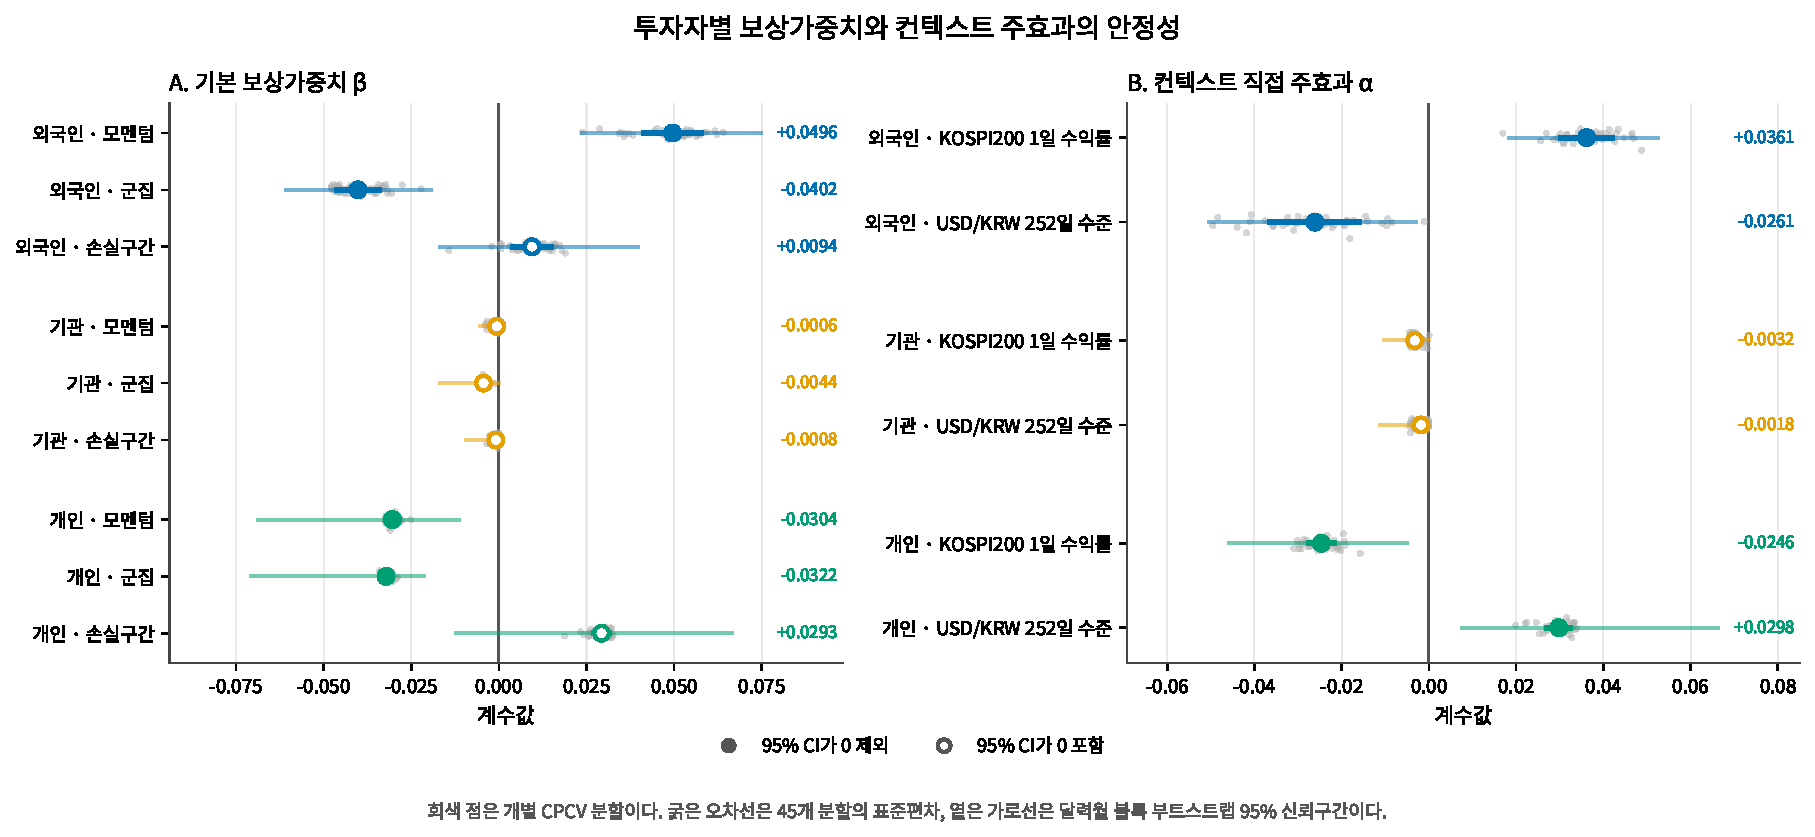
\includegraphics[width=\textwidth]{../figures_v2/fig3_beta_alpha_forest.pdf}
  \caption{Split-level stability of reward weights and context main effects.
  Grey dots are individual CPCV splits, thick error bars the standard deviation
  across the 45 splits, and light horizontal lines the 95\% calendar-month block
  bootstrap interval. Hollow markers denote terms whose interval contains zero.}
  \Description{Forest plots for baseline reward weights (panel A) and context
  main effects (panel B), showing per-split estimates and confidence intervals
  for each term.}
  \label{fig:forest}
\end{figure*}

Figure~\ref{fig:betabar} places the recovered baseline reward weights of the
three types side by side. Because all types received the same feature set and
the same model form and only their parameters were estimated separately, the
differences in bar height are entirely learned from the data.
Figure~\ref{fig:forest} unfolds the same $\beta$ together with the context main
effects $\alpha$ down to the split level.

\paragraph{The mirror image on the momentum axis}
The foreign momentum weight is $+0.0496$ and positive in all 45 splits, while
the retail weight is $-0.0304$ and negative in all 45 splits. In
Figure~\ref{fig:betabar} the two bars point in opposite directions across the
zero line, and in Figure~\ref{fig:forest} their bootstrap intervals do not
overlap and each excludes zero. Although the same feature set was estimated
independently for each type, the two types diverge in exactly opposite
directions on momentum: foreign investors appear as trend followers and retail
investors as contrarians, matching the sign expectations of prior
work~\cite{grinblatt2000investment,choe1999foreign}.

\paragraph{Herding}
The herding coefficient is negative in all 45 splits for all three types, and
the bootstrap intervals of the foreign ($-0.0402$) and retail ($-0.0322$)
coefficients also exclude zero. This result, however, does not separate a
behavioural interpretation from the market-clearing constraint. As
Figure~\ref{fig:crossinv} shows, the same-day correlation between types reaches
$-0.77$, so a substantial part of the negative herding coefficient may arise
mechanically. Because Equation~\eqref{eq:herd} uses a one-day lag the same-day
constraint does not apply directly, but it can propagate through the
autocorrelation of the action. We therefore restrict this result to the
descriptive statement that observed aggregate flow displays a negative
cross-type association, and do not extend it to the behavioural claim that each
type independently trades against the others.

\paragraph{Underwater}
The retail underwater weight is $+0.0293$ and positive in all 45 splits: buying
intensity rises on the following day when the traded price is below the
average-cost proxy, consistent with the reference-price dependence of the
disposition-effect literature~\cite{shefrin1985disposition,odean1998investors}.
The foreign coefficient shares the sign at $+0.0094$ (95.6\%) but is about a
third of the retail magnitude.

As Figure~\ref{fig:forest} shows, however, the underwater bootstrap interval
contains zero for all three types. The retail interval is
$[-0.0122,+0.0665]$: although the sign is 100\% consistent across the 45 splits,
it flips in 5.5\% of month-block resamples. This is exactly the situation
anticipated in \S\ref{sec:protocol}, where sign consistency understates
uncertainty because CPCV splits share observations. We therefore report that a
sign consistent with the disposition effect was observed, but do not claim it as
a statistically established result.

\subsection{Context Response: The Mirror Image Reappears}
\label{sec:alpha}

The mirror image observed on the momentum axis reappears in the context main
effects (panel B of Figure~\ref{fig:forest}). Foreign investors shift toward net
buying on days when the market rises ($+0.0361$) and toward net selling when the
won is weak ($-0.0261$), while retail investors do exactly the opposite on both
contexts ($-0.0246$ and $+0.0298$). All four coefficients keep their sign in all
45 splits and all four bootstrap intervals exclude zero. The two institutional
coefficients have sign consistency above 95\% but are about an eighth of the
foreign and retail magnitudes, and their intervals contain zero.

This mirror image requires the same interpretive reservation as the herding
coefficient. Given the $-0.772$ correlation in Figure~\ref{fig:crossinv}, two
types responding to context with opposite signs may in part reflect the
market-clearing constraint. We therefore present this as the descriptive fact
that the two types form opposite sides of order flow across market and exchange
rate conditions.

\paragraph{Interactions}
Of the twelve interaction coefficients, four keep their sign in all 45 splits:
foreign momentum $\times$ KOSPI200 ($-0.0139$), retail momentum $\times$ FX
($+0.0144$), retail herding $\times$ KOSPI200 ($-0.0080$) and retail
underwater $\times$ FX ($-0.0186$). Only the first and the last of these pass
the bootstrap. Since twelve coefficients were examined jointly, we present the
interactions as exploratory results only.

\subsection{Results of the Stability Protocol}
\label{sec:stability}

\paragraph{(V2) Calendar-month block bootstrap}
The light horizontal lines in Figure~\ref{fig:forest} give this result. The
bootstrap is a stricter criterion than CPCV sign consistency, and the outcome
splits three ways. First, the momentum mirror and the context mirror survive:
eight terms, comprising foreign and retail momentum, herding, and both context
main effects, all exclude zero. Second, the underwater weights do not survive.
Third, no institutional term excludes zero; all six institutional markers in
Figure~\ref{fig:forest} are hollow.

\begin{figure*}[t]
  \centering
  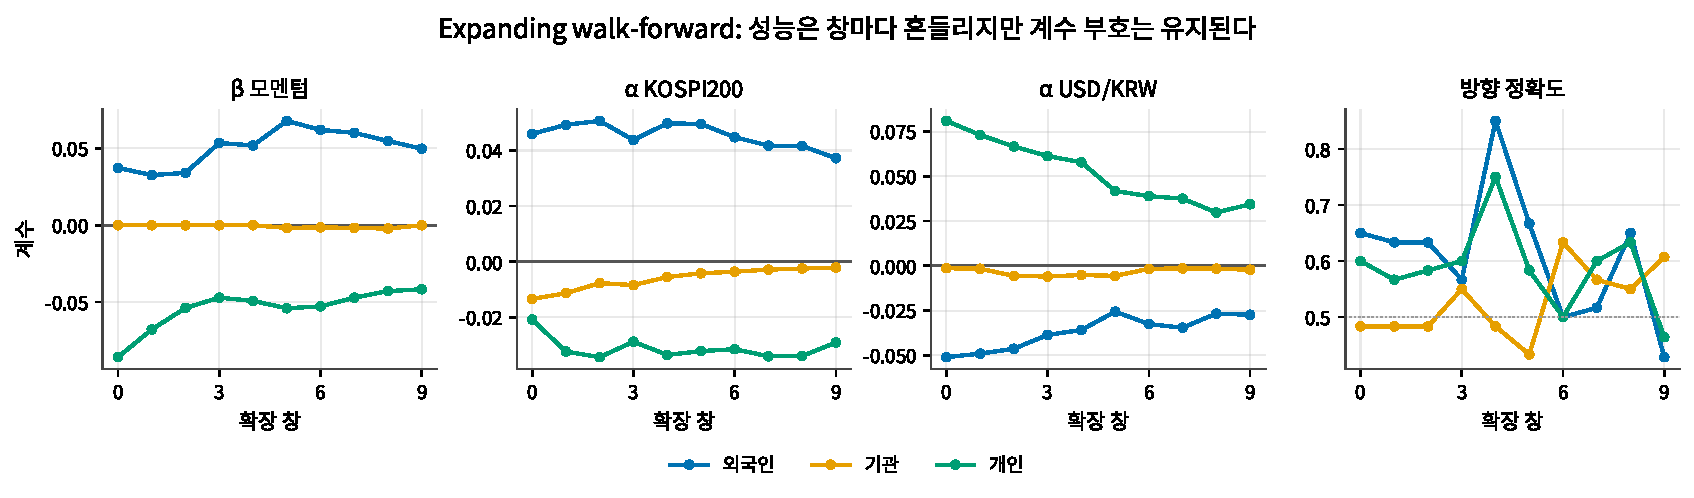
\includegraphics[width=\textwidth]{../figures_v2/fig6_walk_forward.pdf}
  \caption{Coefficient paths and directional accuracy over ten expanding
  walk-forward windows. Performance fluctuates from window to window while the
  coefficient signs hold.}
  \Description{Four line charts against the expanding-window index showing the
  momentum coefficient, the two context main effects, and directional accuracy
  for the three investor types.}
  \label{fig:walkforward}
\end{figure*}

\paragraph{(V3) Expanding walk-forward}
Figure~\ref{fig:walkforward} gives this result, and two things read at once.
Performance fluctuates sharply across windows: foreign directional accuracy
moves between 0.43 and 0.85, averaging $0.610\pm0.116$, and the correlation
falls to $0.131\pm0.162$, less than half the CPCV value of 0.278; retail falls
from 0.245 to 0.129. Because CPCV can place a test fold ahead of a training fold
while walk-forward cannot, we report this degradation as a generalization limit
arising from the temporal structure.

The coefficient paths, by contrast, do not fluctuate. The foreign momentum
coefficient is positive in all ten windows and the retail one negative in all
ten, and the two paths never cross. The same mirror image persists across all
windows for both context main effects, while the three institutional paths stay
pinned near zero. Performance moves with time; the direction of the recovered
preference does not.

\begin{figure*}[t]
  \centering
  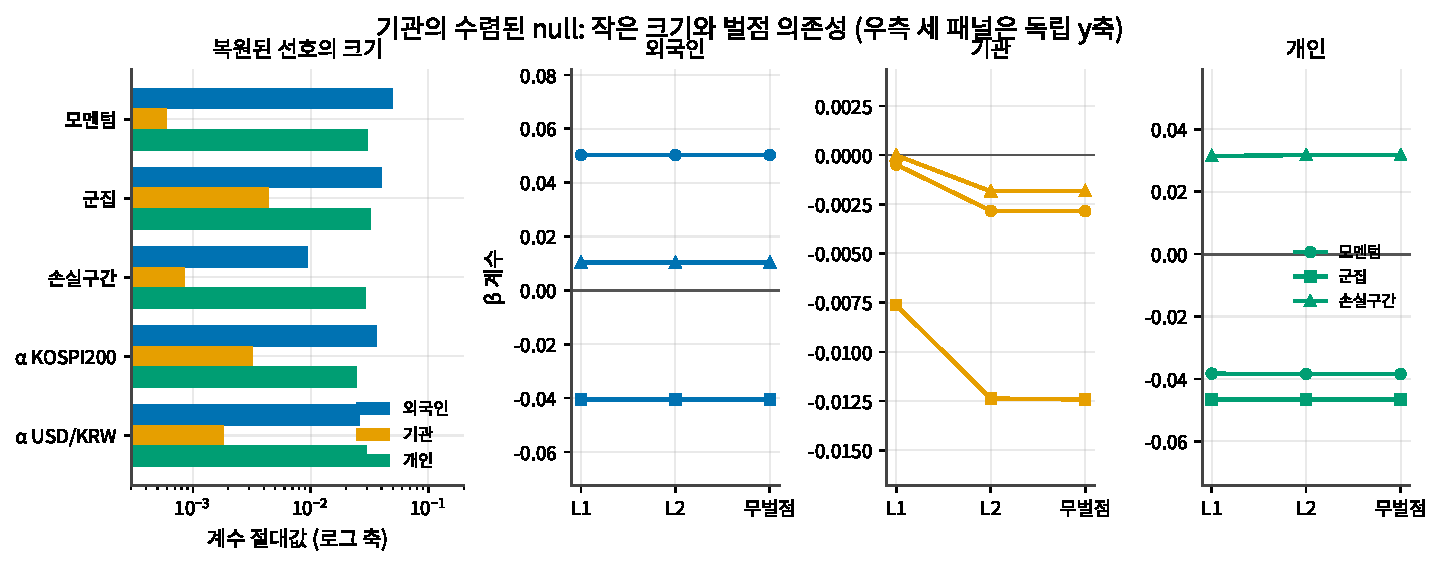
\includegraphics[width=\textwidth]{../figures_v2/fig7_institution_null.pdf}
  \caption{The converged institutional null. Left: magnitude of the recovered
  preferences on a logarithmic axis. Right: sensitivity to the regularization
  swap, with an independent $y$ axis in each of the three panels.}
  \Description{A logarithmic bar chart of coefficient magnitudes by type on the
  left, and three line charts of coefficients under L1, L2 and no penalty on the
  right.}
  \label{fig:null}
\end{figure*}

\paragraph{(V4) Regularization swap}
Figure~\ref{fig:null} gives this result. The foreign and retail coefficients are
effectively invariant to the choice of penalty, agreeing to four decimal places,
so the momentum mirror is not an artefact of the $L_1$ penalty. Only the
institutional coefficients move with the penalty (herding
$-0.0076\rightarrow-0.0124$, underwater $-0.0000\rightarrow-0.0018$), on a
$y$-axis range about one twentieth of that of the other two types. That the
coefficients depend on the choice of penalty means the data do not determine
their value.

\subsection{Institutional Investors: A Converged Null}
\label{sec:null}

For institutional order flow we find no preference that is stably identified at
daily frequency, and we report this as a finding rather than concealing it. The
evidence is fivefold and all of it is visible in the figures.

\begin{enumerate}
\item \textbf{Degenerate prediction.} In the middle panel of
Figure~\ref{fig:prediction} the institutional prediction stays on the zero line
while the actual series moves between $\pm0.1$.
\item \textbf{Magnitude.} In Figure~\ref{fig:betabar} the three institutional
bars are barely visible on the shared axis. Excluding herding, momentum is
$-0.0006$ and underwater $-0.0008$, about one fortieth of the other types.
\item \textbf{Uncertainty.} All six institutional markers in
Figure~\ref{fig:forest} are hollow.
\item \textbf{Penalty dependence.} In the middle right panel of
Figure~\ref{fig:null}, only the institutional coefficients move with the
penalty.
\item \textbf{Temporal instability.} In Figure~\ref{fig:walkforward} the
institutional paths hug the zero line; momentum sign consistency is 40\% of ten
windows and underwater 0\%.
\end{enumerate}

\begin{figure*}[t]
  \centering
  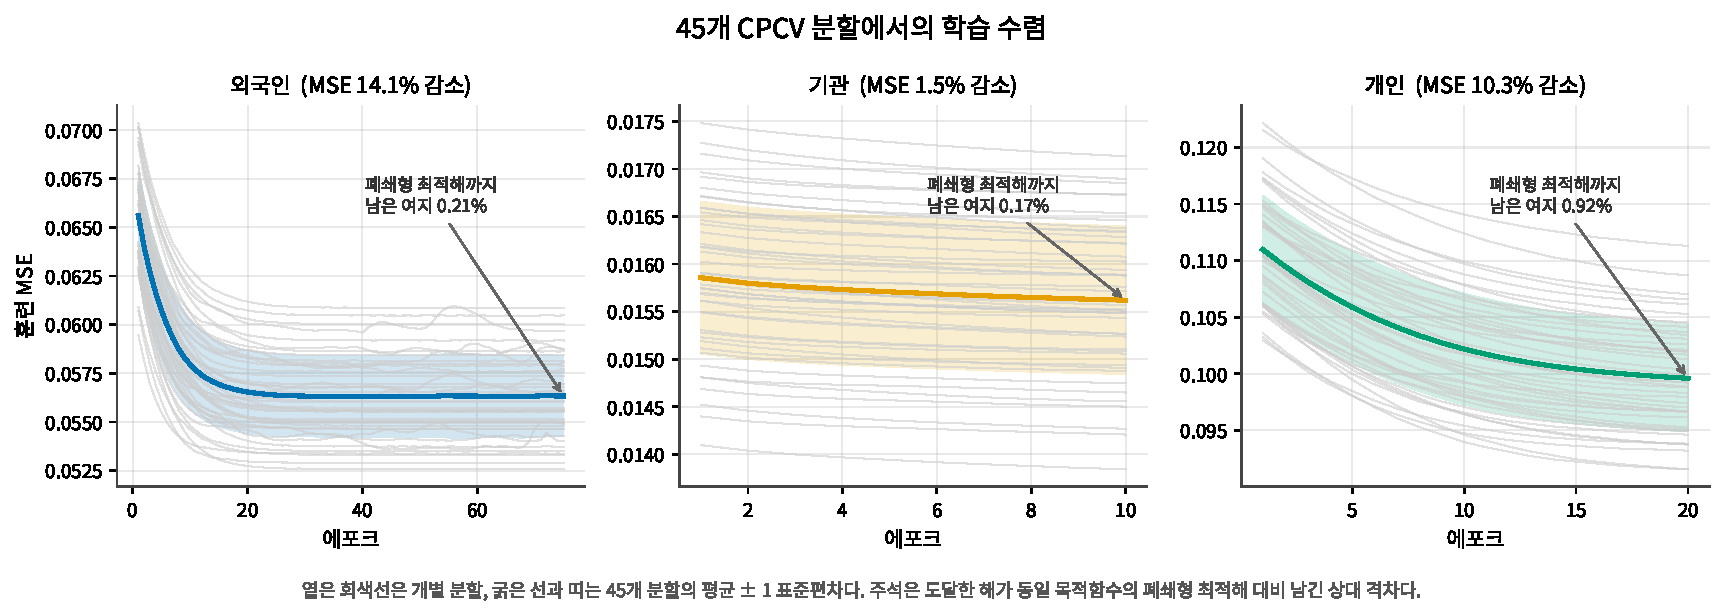
\includegraphics[width=\textwidth]{../figures_v2/fig4_training_convergence.pdf}
  \caption{Training convergence across the 45 CPCV splits. Light grey lines are
  individual splits; the thick line and band are the mean $\pm$ one standard
  deviation. The annotation gives the relative gap between the solution reached
  and the closed-form optimum of the same objective.}
  \Description{Three panels of training MSE against epoch for the three investor
  types; the institutional panel shows the smallest decrease.}
  \label{fig:convergence}
\end{figure*}

This null is not an optimization failure. Figure~\ref{fig:convergence} shows the
training curves across the 45 splits. The institutional training MSE falls by
only 1.5\% over the whole training run and the curve does not look visually
flat. That is not underfitting, however, but the fact that there is almost no
error left to remove. By Proposition~\ref{prop:lasso}, Equation~\eqref{eq:loss}
is convex with a unique global optimum, and comparing the solution reached with
the closed-form optimum of the same objective leaves an institutional gap of
only 0.17\% on average and 0.48\% at most (0.21\% for foreign and 0.92\% for
retail). All three types reach the attainable optimum; only for institutional
investors do the coefficients at that optimum sit near zero. The data do not
determine an institutional preference; it is not that the optimizer failed to
find one.

Economically the null reads naturally. The ``institutional'' category aggregates
pension funds, investment trusts, insurers, private funds, and securities firms,
so the flows of agents with different objective functions offset one another.
The one consistently negative herding coefficient is compatible with a shared
liquidity-provision role on the opposite side of the other types, but because
its bootstrap interval sits on the boundary we do not claim it.

\subsection{Construct Validity Check}
\label{sec:construct}

\begin{table}[t]
  \caption{Prior sign expectations and recovered results}
  \label{tab:construct}
  \small
  \begin{tabular}{@{}>{\raggedright\arraybackslash}p{0.26\columnwidth}
                  >{\raggedright\arraybackslash}p{0.14\columnwidth}
                  >{\raggedright\arraybackslash}p{0.24\columnwidth}
                  >{\raggedright\arraybackslash}p{0.20\columnwidth}@{}}
    \toprule
    Regularity & Expected & Recovered & Verdict \\
    \midrule
    Foreign trend trading~\cite{grinblatt2000investment,choe1999foreign}
      & $\beta^{mom}>0$ & $+0.0496$ (100\%, CI excl.\ 0) & matches \\
    Retail contrarian trading~\cite{grinblatt2000investment,kaniel2008individual}
      & $\beta^{mom}<0$ & $-0.0304$ (100\%, CI excl.\ 0) & matches \\
    Disposition effect~\cite{shefrin1985disposition,odean1998investors}
      & $\beta^{uw}>0$ & $+0.0293$ (100\%, CI incl.\ 0) & partial \\
    Institutional herding~\cite{lakonishok1992impact}
      & $\beta^{herd}>0$ & $-0.0044$ (100\%, CI incl.\ 0) & mismatch \\
    \bottomrule
  \end{tabular}
\end{table}

Table~\ref{tab:construct} reports the contrast. Although all three types
received the same features and the same model form and only their parameters
were estimated separately, the recovered signs agree with independently
established regularities and the two types diverge in opposite directions on
momentum. This is evidence of construct validity: the recovered reward is not an
arbitrary fit.

The mismatch arises because the measured object differs. Lakonishok et
al.~\cite{lakonishok1992impact} measure the extent to which agents \emph{within}
the institutional group move in the same direction, whereas
Equation~\eqref{eq:herd} measures whether institutions move with the previous
day's flow of the \emph{other two types}. Our result is therefore not a
refutation of that literature; testing within-type herding would require data on
institutional sub-categories.

\subsection{What This Study Does Not Claim}
\label{sec:notclaim}

As the final stage of the protocol we state explicitly what the results do not
support.

\begin{enumerate}
\item \textbf{Return predictability.} Our metrics are reproduction errors for
the direction and intensity of order flow and include no returns, Sharpe ratios,
or transaction costs. No trading rule follows from
Table~\ref{tab:performance}.

\item \textbf{Superior flow prediction.} As reported in
Table~\ref{tab:performance} and Figure~\ref{fig:oos}, the persistence baseline
beats the main model on directional accuracy and correlation. Our objective is
preference recovery on an interpretable common scale rather than predictive
performance, and the two objectives call for different feature sets. In a
preliminary check, adding the lagged own action as a fourth feature lifts the
model above the baseline (directional accuracy $0.646/0.569/0.629$) but reverses
the sign of the retail $\alpha^{KOSPI}$ and eliminates the underwater
coefficient. Some of the mirror images reported here are therefore not separable
from the autocorrelation of order flow.

\item \textbf{Causal effects.} The recovered weights are conditional
associations among standardized observed features. Because feature--context
correlations range from $-0.29$ to $0.22$ (Figure~\ref{fig:featcorr}), the
magnitude of any coefficient depends on the other terms being controlled for.

\item \textbf{A behavioural reading of the negative cross-type association.} The
herding coefficient and the mirrored context responses are not separable from
the market-clearing constraint (Figure~\ref{fig:crossinv}).

\item \textbf{A test of the disposition effect.} The retail underwater sign
agrees with the literature but does not pass the month-block bootstrap
(Figure~\ref{fig:forest}), and the average-cost proxy is built from aggregate
trades rather than account-level realized gains and holding periods.

\item \textbf{Generalization across stocks.} The single-stock design is a
control for isolating heterogeneity across types; extension to other stocks and
markets is untested.
\end{enumerate}

% =====================================================================
\appendix

\section{Supplementary Material}
\label{sec:appendix}

This appendix collects the supporting figures and tables referenced in the main
text. Figure~\ref{fig:saturation} verifies the premise of
Proposition~\ref{prop:lasso}, Figure~\ref{fig:featcorr} reports
feature--context correlations, and Figure~\ref{fig:crossinv} shows same-day
actions across types. Table~\ref{tab:interactions} lists the full set of
interaction coefficients presented as exploratory in the main text, and
Table~\ref{tab:convergence} reports the optimality check of the solution
reached.

\begin{figure}[htbp]
  \centering
  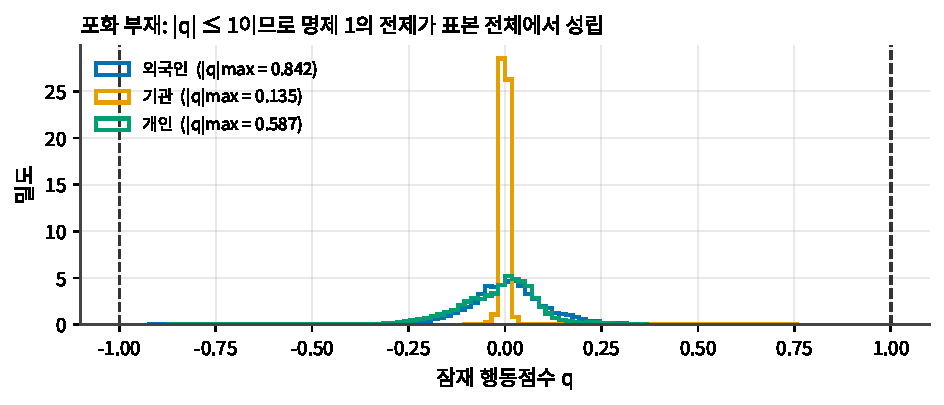
\includegraphics[width=\columnwidth]{../figures_v2/figA1_no_saturation.pdf}
  \caption{Distribution of the latent action score against the action bounds.
  Since $|q|\le1$, the premise of Proposition~\ref{prop:lasso} holds throughout
  the sample and the saturation rate is exactly zero in all 45 splits.}
  \Description{Histograms of the latent action score for the three types with
  the $\pm1$ bounds marked.}
  \label{fig:saturation}
\end{figure}

\begin{figure}[htbp]
  \centering
  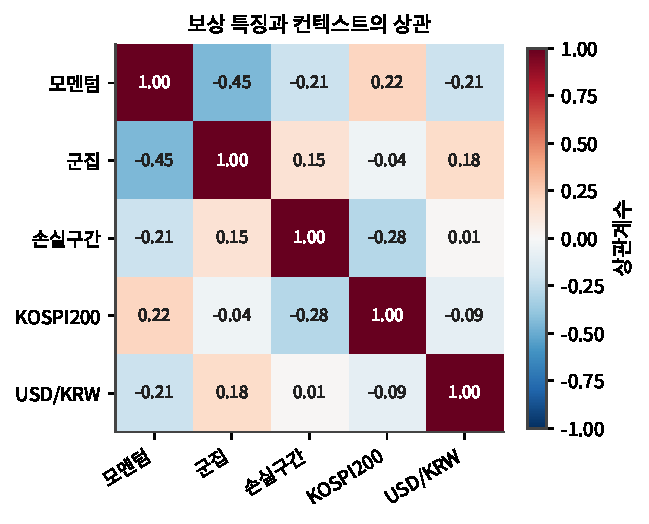
\includegraphics[width=\columnwidth]{../figures_v2/figA2_feature_correlation.pdf}
  \caption{Correlation matrix of reward features and contexts (foreign features,
  973 observations).}
  \Description{A heatmap showing correlation coefficients among five variables
  in colour and numerals.}
  \label{fig:featcorr}
\end{figure}

\begin{figure}[htbp]
  \centering
  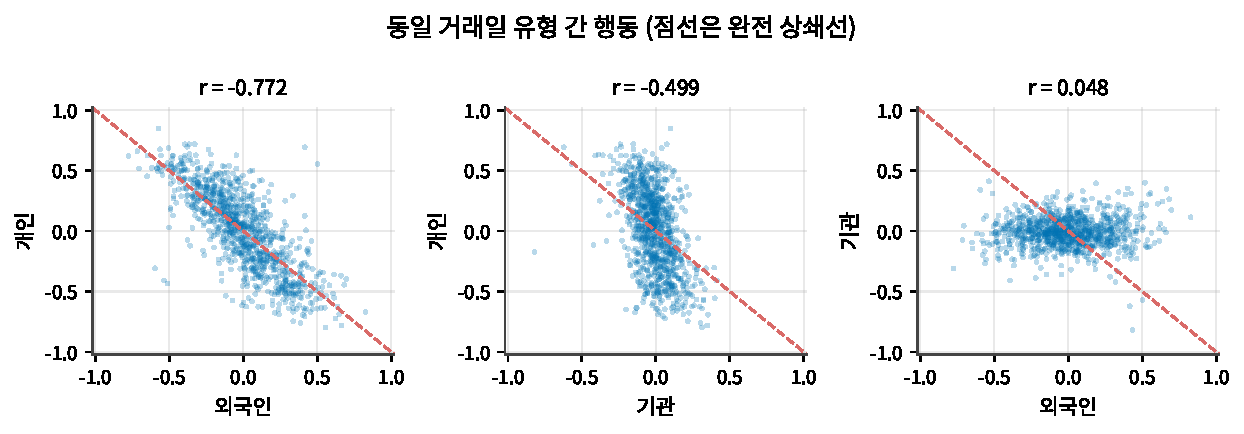
\includegraphics[width=\columnwidth]{../figures_v2/figA3_cross_investor_actions.pdf}
  \caption{Same-day actions across investor types. The dashed line marks perfect
  offset; foreign and retail actions cluster along it.}
  \Description{Three scatter plots of actions for each pair of investor types
  with the corresponding correlation coefficients.}
  \label{fig:crossinv}
\end{figure}

\begin{table}[htbp]
  \caption{Interaction coefficients $B$ (45 splits)}
  \label{tab:interactions}
  \small
  \centering
  \begin{tabular}{@{}llrrr@{}}
    \toprule
    Type & Feature $\times$ context & Mean & S.d. & Sign cons. \\
    \midrule
    Foreign & momentum $\times$ KOSPI200 & $-0.0139$ & $0.0052$ & 100.0\% \\
    Foreign & momentum $\times$ FX       & $-0.0030$ & $0.0057$ & 71.1\% \\
    Foreign & herding $\times$ KOSPI200  & $+0.0016$ & $0.0074$ & 66.7\% \\
    Foreign & herding $\times$ FX        & $+0.0037$ & $0.0073$ & 68.9\% \\
    Foreign & underwater $\times$ KOSPI200 & $-0.0062$ & $0.0040$ & 93.3\% \\
    Foreign & underwater $\times$ FX     & $-0.0075$ & $0.0076$ & 86.7\% \\
    \addlinespace
    Inst. & momentum $\times$ KOSPI200 & $-0.0001$ & $0.0005$ & 66.7\% \\
    Inst. & momentum $\times$ FX       & $+0.0003$ & $0.0006$ & 80.0\% \\
    Inst. & herding $\times$ KOSPI200  & $-0.0004$ & $0.0006$ & 86.7\% \\
    Inst. & herding $\times$ FX        & $+0.0012$ & $0.0012$ & 93.3\% \\
    Inst. & underwater $\times$ KOSPI200 & $+0.0028$ & $0.0012$ & 97.8\% \\
    Inst. & underwater $\times$ FX     & $+0.0007$ & $0.0008$ & 91.1\% \\
    \addlinespace
    Retail & momentum $\times$ KOSPI200 & $+0.0021$ & $0.0042$ & 80.0\% \\
    Retail & momentum $\times$ FX       & $+0.0144$ & $0.0045$ & 100.0\% \\
    Retail & herding $\times$ KOSPI200  & $-0.0080$ & $0.0046$ & 100.0\% \\
    Retail & herding $\times$ FX        & $+0.0092$ & $0.0081$ & 82.2\% \\
    Retail & underwater $\times$ KOSPI200 & $-0.0022$ & $0.0046$ & 66.7\% \\
    Retail & underwater $\times$ FX     & $-0.0186$ & $0.0046$ & 100.0\% \\
    \bottomrule
  \end{tabular}
\end{table}

\begin{table}[htbp]
  \caption{Optimality check of the solution reached (45 splits)}
  \label{tab:convergence}
  \small
  \centering
  \begin{tabular}{@{}lccc@{}}
    \toprule
    Type & MSE drop & Gap (\%) & Cosine \\
     & (training) & mean / max & mean / min \\
    \midrule
    Foreign & 14.1\% & $0.21/3.10$ & $0.994/0.948$ \\
    Inst.   & 1.5\%  & $0.17/0.48$ & $0.935/0.832$ \\
    Retail  & 10.3\% & $0.92/1.40$ & $0.894/0.833$ \\
    \bottomrule
  \end{tabular}
\end{table}
